%# -*- coding: utf-8-unix -*-
%%==================================================
%% thesis.tex
%%==================================================

% 双面打印
\documentclass[master, fontset=adobe, openright, twoside, openany, zihao=-4]{sjtuthesis}
% \documentclass[bachelor, fontset=adobe, openany, oneside, submit]{sjtuthesis}
% \documentclass[master, fontset=adobe, review]{sjtuthesis}
% \documentclass[%
%   bachelor|master|doctor,	% 必选项
%   fontset=adobe|windows,  	% 只测试了adobe
%   oneside|twoside,		% 单面打印,双面打印(奇偶页交换页边距,默认)
%   openany|openright, 		% 可以在奇数或者偶数页开新章|只在奇数页开新章(默认)
%   zihao=-4|5,, 		% 正文字号:小四、五号(默认)
%   review,	 		% 盲审论文,隐去作者姓名、学号、导师姓名、致谢、发表论文和参与的项目
%   submit			% 定稿提交的论文,插入签名扫描版的原创性声明、授权声明 
% ]

% 逐个导入参考文献数据库
\addbibresource{bib/thesis.bib}
% \addbibresource{bib/chap2.bib}

\begin{document}

%% 无编号内容:中英文论文封面、授权页
%# -*- coding: utf-8-unix -*-
\title{SSD缓存系统的设计与实现}
\author{傅雨东}
\advisor{李小勇}
% \coadvisor{某某教授}
\defenddate{2018年1月15日}
\school{上海交通大学}
\institute{网络空间安全学院}
\studentnumber{115036910016}
\major{计算机科学与技术}

\englishtitle{The Design and Implement of Solid State Disk Cache System}
\englishauthor{\textsc{Fu Yudong}}
\englishadvisor{\textsc{Li Xiaoyong}}
% \englishcoadvisor{Prof. \textsc{Uom Uom}}
\englishschool{Shanghai Jiao Tong University}
\englishinstitute{\textsc{School of Cyber Security} \\
  \textsc{Shanghai Jiao Tong University} \\
  \textsc{Shanghai, P.R.China}}
\englishmajor{Computer Science and Technolgy}
\englishdate{Jan. 15th, 2018}


\maketitle

\makeenglishtitle

\makeatletter
\ifsjtu@submit\relax
	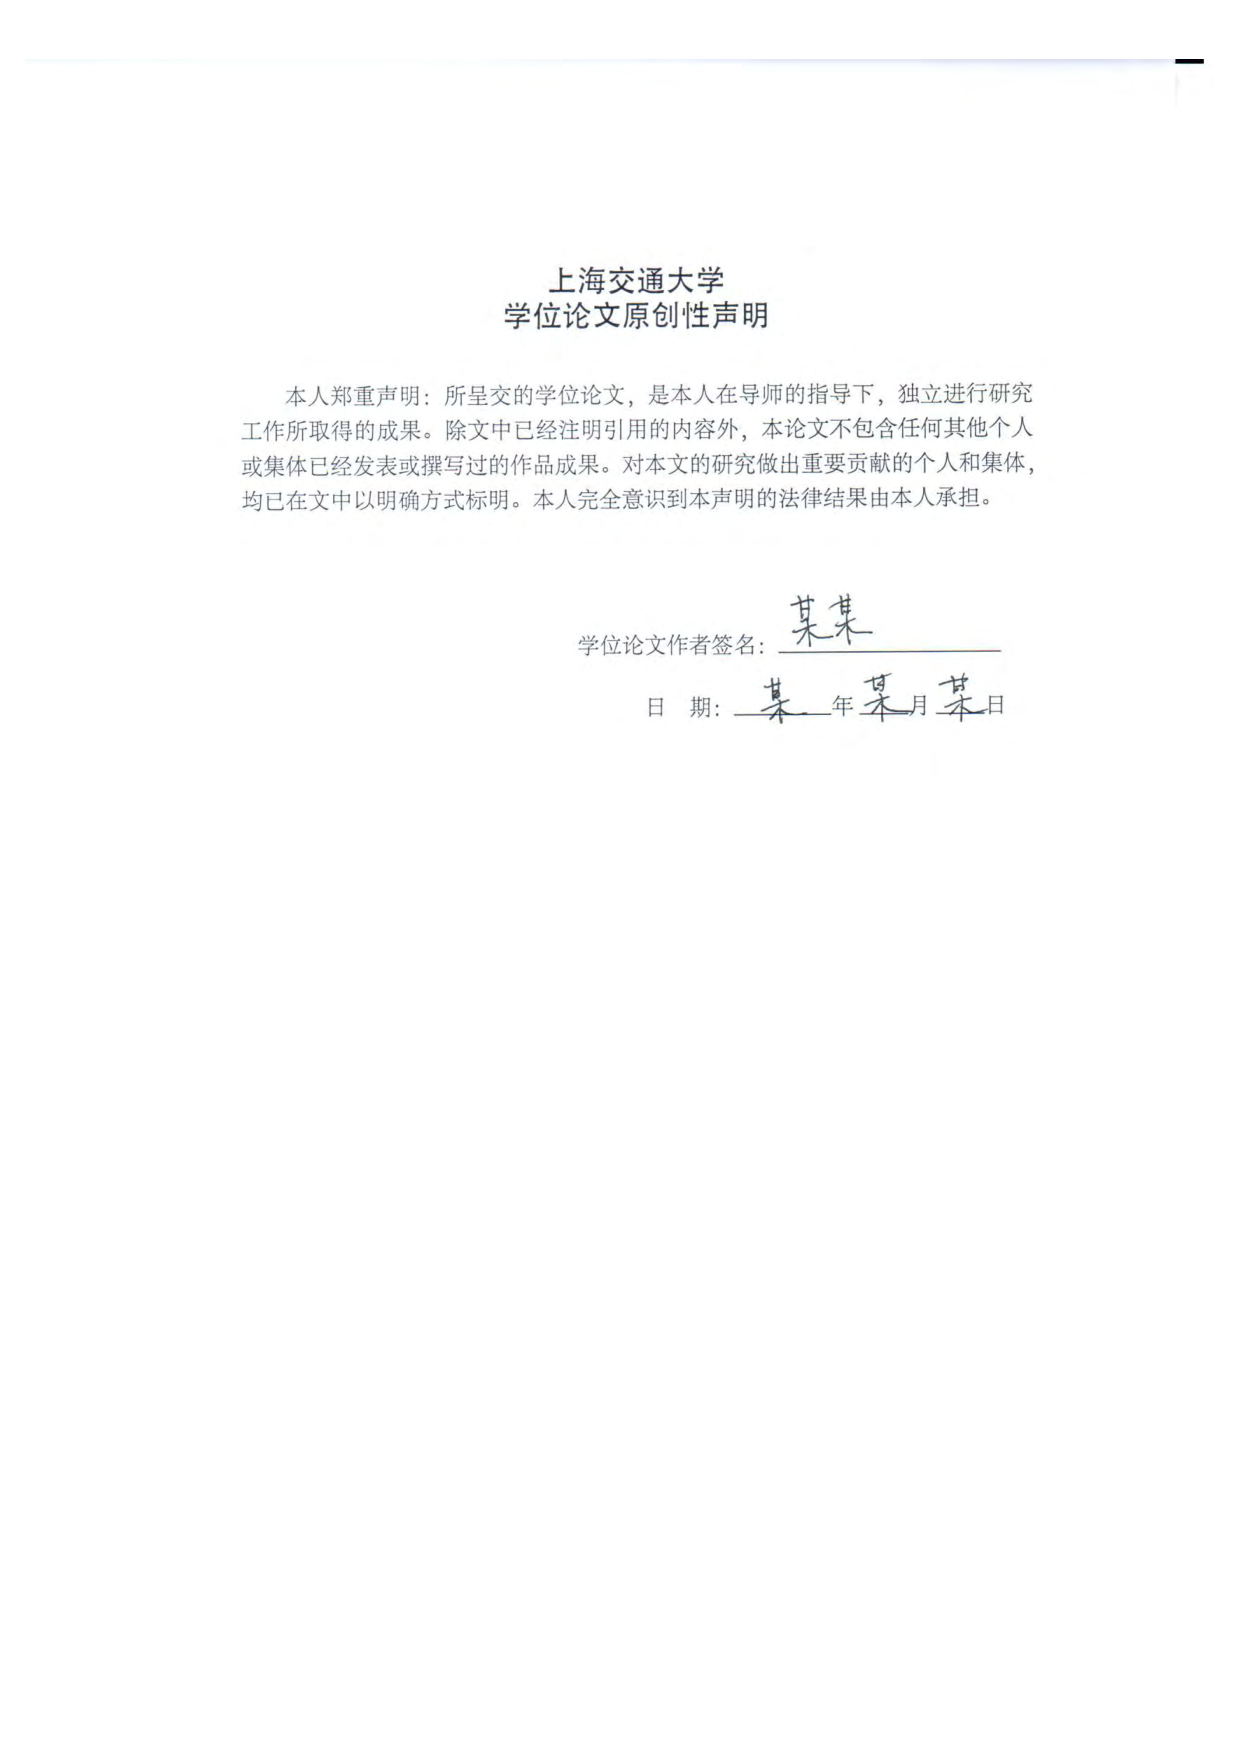
\includepdf{pdf/original.pdf}
	\cleardoublepage
	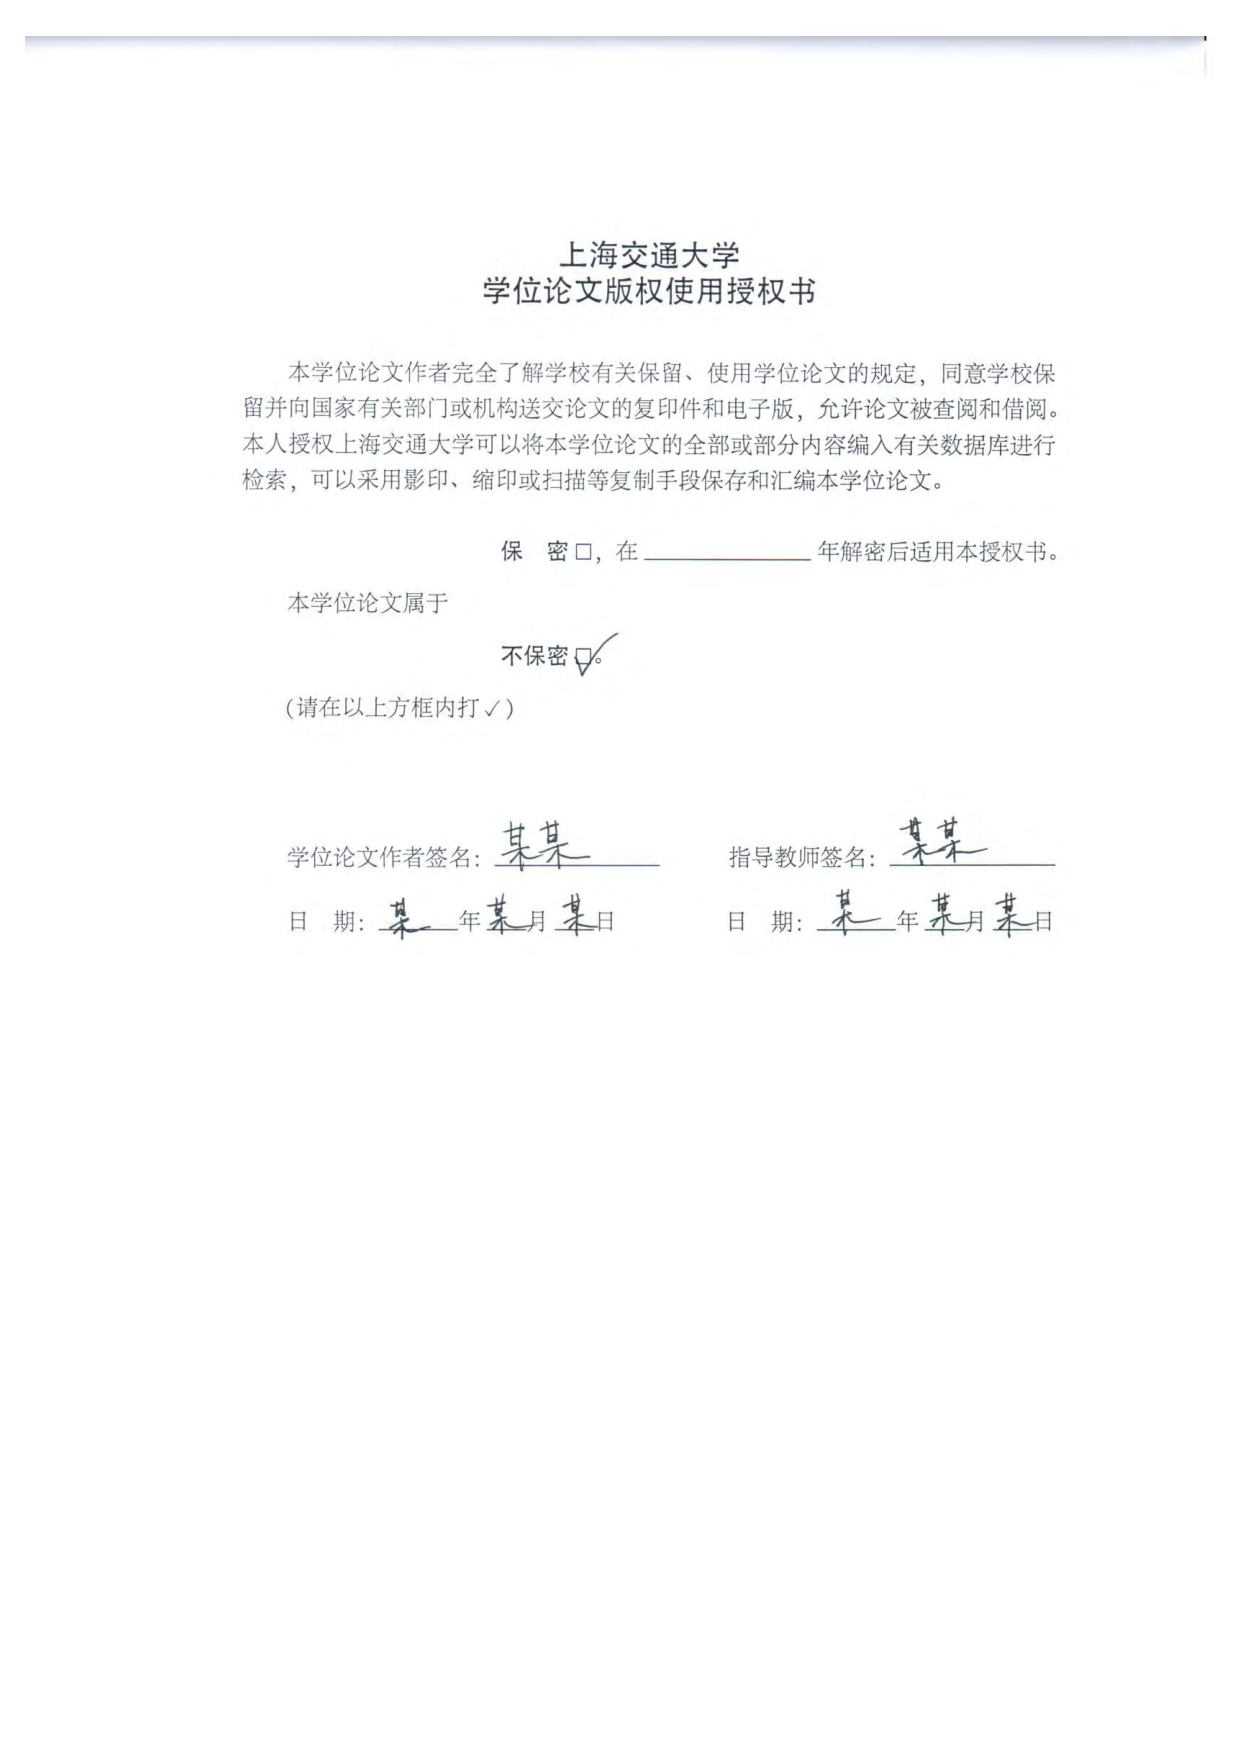
\includepdf{pdf/authorization.pdf}
	\cleardoublepage
\else
\ifsjtu@review\relax
% exclude the original claim and authorization
\else
	\makeDeclareOriginal
	\makeDeclareAuthorization
\fi
\fi
\makeatother


\frontmatter 	% 使用罗马数字对前言编号

%% 摘要
\pagestyle{main}
%# -*- coding: utf-8-unix -*-
%%==================================================
%% abstract.tex for SJTU Master Thesis
%%==================================================

\begin{abstract}

随着云计算与大数据的快速发展,对作为其基石的存储系统的要求越来越高,存储系统需要具备大容量、低成本、高性能。而目前主流的任何一种存储设备如固态盘、磁盘由于各种限制不能单独构建出同时满足上述要求的存储系统。混合存储系统充分利用不同存储设备特性的互补构建高效的存储系统,既能支持大容量,又能在保证系统低成本下仍能具有高性能,成为目前的研究热点。

本文首先介绍了混合存储系统的基本概念和发展历史,然后研究了混合存储系统在设计中的关键技术,之后研究了三个开源混合存储系统,在此基础上设计并实现了一个基于SSD和HDD的SSD缓存系统qscache。本文的主要工作如下:

\begin{enumerate}
    \item 对当前主流的存储设备介绍,并对性能、成本、容量进行了分析对比。
    \item 对混合存储系统的发展历史进行了研究并分析总结了混合存储系统在设计中的关键技术。
    \item 对三个开源混合存储系统进行了研究,分析对比了它们的性能和特性。
    \item 设计并实现了qscache系统。
    \item 对qscache系统的性能以及多缓存设备对多后台设备功能和对I/O带宽按权限分配的功能进行了测试。
\end{enumerate}

测试结果显示qscache系统的整体性能与flashcache接近,并且成功实现对I/O带宽按权限分配的功能,系统通过Linux内核模块实现,但需要对Linux内核进行修改。本论文的研究成果对于其它的混合存储系统设计与实现以及需要对Linux中Device Mapper进行功能扩展与修改的研究具有较好的借鉴价值。

\keywords{\large 混合存储 \quad 固态盘 \quad 磁盘 \quad 按权限配额}
\end{abstract}

\begin{englishabstract}

With the rapid development of cloud computing and big data, the storage system, which is the cornerstone, needs to provide high storage capacity and high performance at low cost. While at present any one of the storage devices, such as solid state disk and hard disk drive, can not meet the above requirements alone due to various limitations. Hybrid storage system takes full advantage of the characteristics of different storage device to support large-capacity, but also ensures high performance at low cost. Therefore, hybrid storage system is becoming the current research focus. 

This paper introduces the basic concepts and development history of hybrid storage system first, then studies the key technologies in the design of hybrid storage system, and then studies three open source hybrid storage systems, based on which, a hybrid storage system named qscache is designed and implentmented. The main work of this paper is as follows:

\begin{enumerate}
    \item The current wide-used storage devices are introduced, and their performance, cost, capacity were analyzed and compared.
    \item The history of the development of hybrid storage systems was studied and the key technologies in the design of hybrid storage systems were summarized.
    \item Three open source hybrid storage systems were studied, and their performance and characteristics were analyzed and compared.
    \item The design and implementation of hybrid storage system qscache.
    \item The performance of the qscache system, as well as the ability of support of multiple cache devices to multiple backend devices and the support of assigning I / O bandwidth based on weight, was tested.
\end{enumerate}

The test results shows that the performance of the qscache system is close to flashcache, and assigning I / O bandwidth based on weight is implemented. The qscache system is implemented as a kernel module in Linux, but the modification of Linux kernel is a must. This research provides a reference for the design and implementation of other hybrid storage systems and the modification of the Device Mapper in Linux kernel.

\englishkeywords{\large hybrid storage, solid state disk, hard disk drive, weight-based quota}
\end{englishabstract}



%% 目录、插图目录、表格目录
\tableofcontents
\listoffigures
\addcontentsline{toc}{chapter}{\listfigurename} %将插图目录加入全文目录
\listoftables
\addcontentsline{toc}{chapter}{\listtablename}  %将表格目录加入全文目录
\listofalgorithms
\addcontentsline{toc}{chapter}{算法索引}        %将算法目录加入全文目录

%%# -*- coding: utf-8-unix -*-
\chapter{主要符号对照表}
\label{chap:symb}

\begin{longtable}{rl}
$\epsilon$     & 介电常数 \\
 $\mu$ 		& 磁导率 \\
 $\epsilon$     & 介电常数 \\
 $\mu$ 		& 磁导率 \\
 $\epsilon$     & 介电常数 \\
 $\mu$ 		& 磁导率 \\
 $\epsilon$ 	& 介电常数 \\
 $\mu$ 		& 磁导率 \\
 $\epsilon$     & 介电常数 \\
 $\mu$ 		& 磁导率 \\
 $\epsilon$     & 介电常数 \\
 $\mu$ 		& 磁导率 \\
 $\epsilon$     & 介电常数 \\
 $\mu$ 		& 磁导率 \\
 $\epsilon$ 	& 介电常数 \\
 $\mu$ 		& 磁导率 \\
 $\epsilon$     & 介电常数 \\
 $\mu$ 		& 磁导率 \\
 $\epsilon$     & 介电常数 \\
 $\mu$ 		& 磁导率 \\
 $\epsilon$     & 介电常数 \\
 $\mu$ 		& 磁导率 \\
 $\epsilon$ 	& 介电常数 \\
 $\mu$ 		& 磁导率 \\
 $\epsilon$     & 介电常数 \\
 $\mu$ 		& 磁导率 \\
 $\epsilon$     & 介电常数 \\
 $\mu$ 		& 磁导率 \\
 $\epsilon$     & 介电常数 \\
 $\mu$ 		& 磁导率 \\
 $\epsilon$ 	& 介电常数 \\
 $\mu$ 		& 磁导率 \\
 $\epsilon$     & 介电常数 \\
 $\mu$ 		& 磁导率 \\
 $\epsilon$     & 介电常数 \\
 $\mu$ 		& 磁导率 \\
 $\epsilon$     & 介电常数 \\
 $\mu$ 		& 磁导率 \\
 $\epsilon$ 	& 介电常数 \\
 $\mu$ 		& 磁导率 \\
 $\epsilon$     & 介电常数 \\
 $\mu$ 		& 磁导率 \\
 $\epsilon$     & 介电常数 \\
 $\mu$ 		& 磁导率 \\
 $\epsilon$     & 介电常数 \\
 $\mu$ 		& 磁导率 \\
 $\epsilon$ 	& 介电常数 \\
 $\mu$ 		& 磁导率 \\
 $\epsilon$     & 介电常数 \\
 $\mu$ 		& 磁导率 \\
 $\epsilon$     & 介电常数 \\
 $\mu$ 		& 磁导率 \\
 $\epsilon$     & 介电常数 \\
 $\mu$ 		& 磁导率 \\
\end{longtable}
 % 主要符号、缩略词对照表

\mainmatter	% 使用阿拉伯数字对正文编号

%% 正文内容
\pagestyle{main}
%# -*- coding: utf-8-unix -*-
%%==================================================
%% chapter01.tex for SJTU Master Thesis
%%==================================================

%\bibliographystyle{sjtu2}%[此处用于每章都生产参考文献]
\chapter{绪论}
\label{chap:intro}

\section{研究背景与意义}

\subsection{研究背景}
\label{sec:backgrounds}

大规模分布式存储系统是是云计算与大数据的基石,是近年来的研究热点。随着近年来云计算与大数据的兴起,现有的存储设备正面临着诸多挑战。首先,随着数据量的爆发式增长,对存储系统的容量提出了更高的要求,如何在提供大容量存储的前提下尽可能降低成本是一大挑战\cite{gray2003next}。其次,由于云计算中的多台虚拟机可能会依赖于同一存储系统,这就导致该存储系统的负载整体会表现为随机化与碎片化,这对存储系统的随机读写性能有很高要求。最后,至今计算性能可谓日益提高,相比最初已有了巨大的提升,但存储设备的读写性能提高仍然有限,这就导致计算性能与存储性能之间的差距越来越巨大\cite{morris2003evolution},如何能提供与计算性能相匹配的存储设备的读写性能也是另一大挑战。

根本上来看,存储系统所基于的存储设备极大地决定了存储系统的性能。目前,磁盘(HDD:Hard Disk Drive)仍然是存储系统中最广泛使用的存储设备,虽然随着各种硬件技术的发展,磁盘的容量依然依照摩尔定律\cite{schirle1996history}在过去的30多年中增长了近十万倍,但是由于其磁头是机械移动这一根本性的限制,磁盘的访问延迟在过去的30年中仅提高了约2倍,而如果通过提高转速来进一步提高磁盘的访问性能,过高的转速会引发能耗与散热等诸多问题,因此磁盘的容量与访问性能之间的鸿沟十分巨大。

近年来,SSD(Solid State Disk,也被称为固态盘)这一新型存储设备的飞速发展为提升存储系统的性能提供了新的研究方向。与磁盘不同,SSD是电子器件,不像磁盘需要磁头的机械移动,因此SSD的随机读写性能要远胜于磁盘,另外由于没有磁头的机械移动,SSD相比磁盘的能耗更低,另外也更具抗震性。然而SSD仍有诸多问题。首先,虽然SSD相比磁盘在随机读写上性能要优秀得多,然而在顺序读写上性能相比磁盘并没有明显的优势。其次,SSD的成本相比磁盘仍要高出许多。最后,SSD的读写性能并不对称,这是由于SSD的写操作造成的,SSD对数据进行更新时需要首先将新数据写入空闲页面,然后将原页面标记为invalid,之后等待将原页面擦除后再将新数据写入原页面,最终导致SSD的写操作耗时约为读操作的6倍,并且由于SSD的擦除操作具有约五万次的次数限制,超出次数后的页面将无法使用,因此会带来耐久性问题。虽然SSD有上述几个问题,但SSD的优缺点与磁盘的优缺点可以很好地互补,因此将SSD与磁盘结合使用为设计大容量、高性能、低成本的存储系统提供了新的可能。

\subsection{研究意义}

目前在学术界与产业界,混合存储系统的研究越发受到重视,各方面的研究都有在开展。但是对于混合存储系统的研究仍然有些问题,主要体现在以下两个方面:

一方面,总的来看,学术界目前对于混合存储系统的研究尚处于起步阶段,很多工作的重点并不在于混合存储系统的设计与实现,而主要在关注SSD的物理结构与特性,关于基于SSD与磁盘的混合存储系统的文献\cite{guerra2011cost, kim2011hybridstore, 杨濮源2012一种时间敏感的, 陈震37基于磁盘和固态硬盘的混合存储系统研究综述}能公开搜索到的很少。另外在少数提出的基于SSD与磁盘的混合存储系统的文献中,真正进行了测试验证的文献更少,更多的是仅仅提供一种思路,无法验证其正确性。产业界中由一些国际一流的存储设备厂商推出的存储产品中已经有开始使用基于SSD与磁盘的混合存储设计,但这些存储设备的内部实现由于厂商并未公开相应资料因而无从知晓,性能的提升仅能依赖于一些简单的测试而并不能得知各项具体的性能提升数值。

另一方面,由于之前提到的SSD的擦除次数限制,这就导致在混合存储系统的写操作面临两难的境地:如果对于数据的写操作都在SSD中进行,那么势必会影响SSD的寿命,而如果将数据的写操作放到磁盘进行,那么势必会影响混合存储系统整体的写性能。因此目前混合存储系统的设计中仍有问题尚待解决。

因此,把握住SSD这一新型存储器件带来的机遇,开展基于SSD与磁盘的混合存储系统的研究,一方面是对于存储系统基础理论的创新,另一方面也对提升我国存储领域的核心竞争力具有重大意义。更进一步,也是为当下以及未来,我国云计算与大数据的发展打下坚实的存储基础。

\section{研究内容与目标}

本文将通过学习存储相关理论,并结合现有的混合存储系统实例分析,研究混合存储系统中的关键技术,在此基础上设计实现以SSD作为磁盘缓存的SSD缓存系统,对其进行测试、完善和优化,并与其它软件进行比较测试。

本文主要将包括以下三大目标:
\begin{enumerate}
    \item SSD、磁盘的随机读写性能、顺序读写性能、容量、成本的对比分析。
    \item 现有混合存储系统的随机读写性能、顺序读写性能、可靠性、额外开销的对比分析。
    \item 混合存储系统设计中的关键技术研究。
    \item 设计并实现一个基于SSD与磁盘的混合存储系统
\end{enumerate}

\section{论文结构}

论文正文分为七个章节,各章的内容安排如下: 

第一章:绪论。给出了论文的研究背景及意义,阐述了论文课题的研究内容和目标,最后说明了论文的组织结构。 

第二章:混合存储系统介绍。介绍了混合存储系统的概念,对当前主流的存储设备的特性进行了介绍,并对混合存储系统的发展历程进行了介绍。 

第三章:混合存储系统设计中的关键技术研究。本章节从系统架构、数据映射策略、冷热数据识别策略、数据写回/迁移策略、最优化存储设备组合这五个方面展开分析了混合存储系统设计中的关键技术。 

第四章:开源混合存储系统介绍。本章节对于目前主流的三个开源的混合存储框架进行了对比分析。

第五章:系统设计。首先介绍了qscache系统的设计目标与设计思想,然后介绍了qscache系统的系统架构、数据映射策略、冷热数据识别策略、数据写回/迁移策略、最优化存储设备组合等设计。 

第六章:系统实现。首先对于系统实现过程中需要掌握的预备知识进行介绍,然后对系统中一些关键问题的具体实现方法进行阐述。 

第七章:系统测试。首先介绍了系统测试的目标与测试方法,然后对于qscache系统的性能与功能进行测试,最后进行了小结。 

第八章:总结与展望。对论文所做的工作进行了总结,并且展望了将来可能的改进工作与改进方向。


%# -*- coding: utf-8-unix -*-
%%==================================================
%% chapter01.tex for SJTU Master Thesis
%%==================================================

%\bibliographystyle{sjtu2}%[此处用于每章都生产参考文献]
\chapter{混合存储系统介绍}
\label{chap:hss_intro}
%# -*- coding: utf-8-unix -*-
%%==================================================
%% chapter01.tex for SJTU Master Thesis
%%==================================================

%\bibliographystyle{sjtu2}%[此处用于每章都生产参考文献]
\chapter{混合存储系统设计中的关键技术研究}
\label{chap:key_tech}

目前,针对基于SDD与HDD的混合存储系统的设计主要从系统架构、数据映射策略、冷热数据识别策略、数据写回/迁移策略、最优化存储设备组合这五个方面展开。

\section{系统架构}

目前基于SSD与HDD的混合存储系统主要有两种系统架构:一种是分层的架构,将SSD作为HDD的缓存;另一种是同层的架构,将SSD与HDD放在同一层,对存储系统而言,SSD与HDD是相对独立的存储设备。

\subsection{分层架构}

分层架构的结构如图\ref{fig:multi_layer_architecture}所示,在该架构下,SSD被完全用作HDD的缓存,混合存储系统的逻辑地址与HDD的物理地址一一对应,当混合存储系统收到来自上层的I/O请求时,首先在SSD中找寻是否存在该数据,如果存在该数据则直接在SSD中对该数据进行操作,否则会去访问HDD进行进一步操作。

在分层架构下,由于SSD比RAM以及NVRAM有更大的容量,因此较RAM与NVRAM可以缓存更多数据,使得系统整体的命中率得到提升,进而提升系统整体的读写性能。然而该架构下仍然要面临被缓存在SSD中的脏数据的处理问题,即是频繁缓存到SSD中提高性能还是频繁写回到HDD中提升SSD的寿命这一两难问题。

\begin{figure}[!htp]
    \centering
    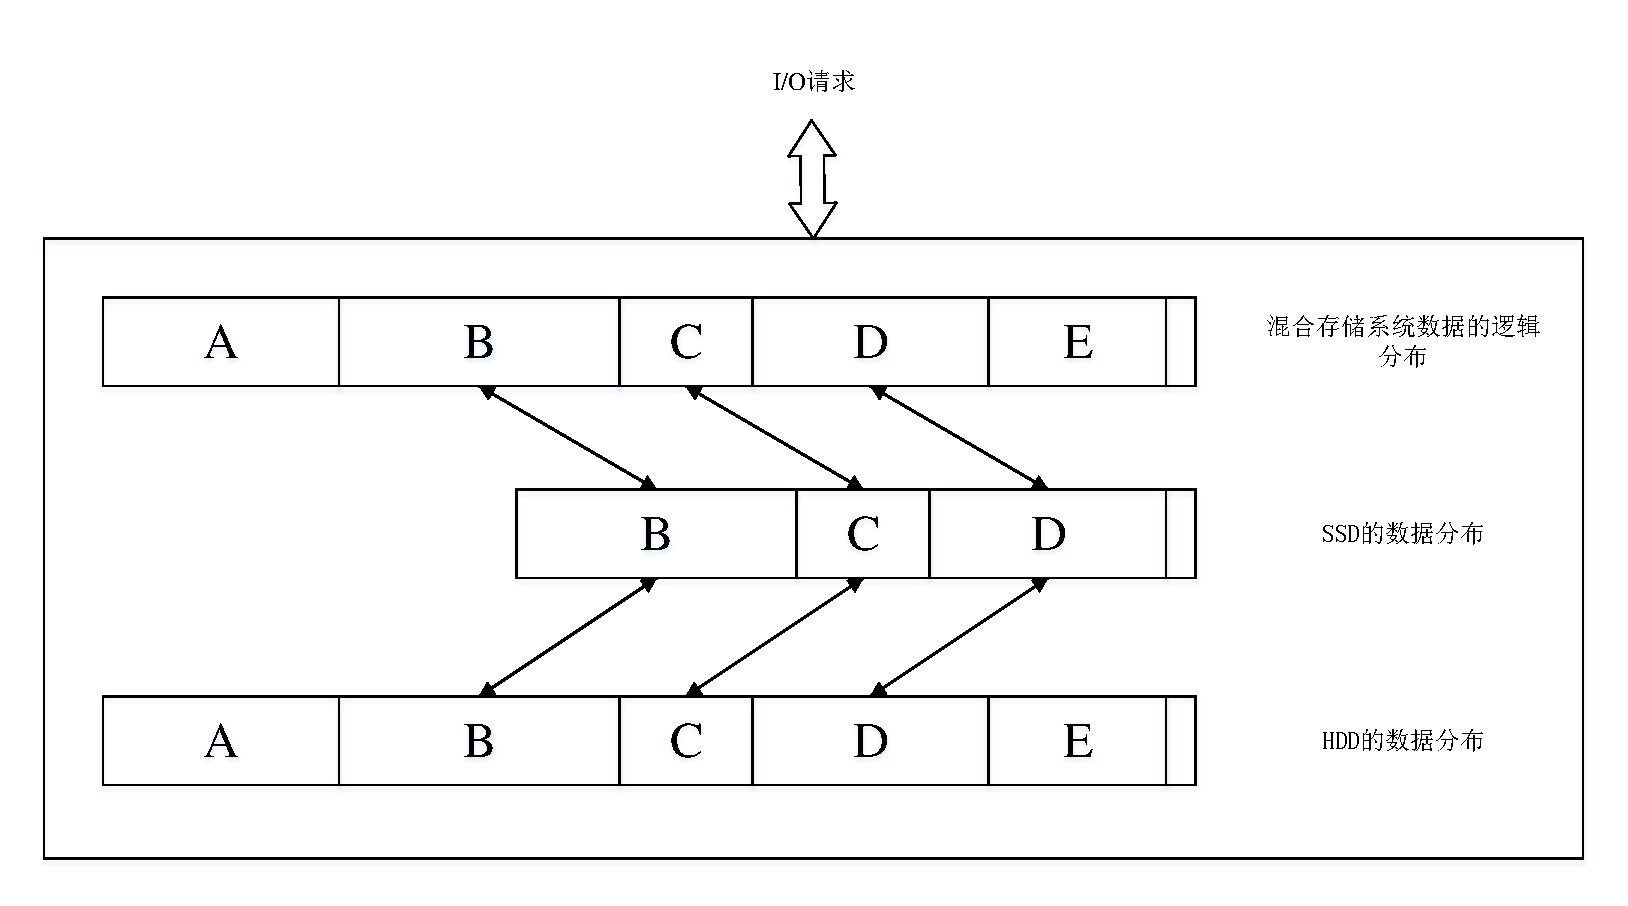
\includegraphics[width=0.8\textwidth]{multi_layer_architecture.pdf}
    \bicaption[fig:multi_layer_architecture]{分层混合存储系统架构}{分层混合存储系统架构}{Fig}{multi-layer hybrid storage system architecture}
\end{figure}

\subsection{同层架构}

同层架构的结构如图\ref{fig:single_layer_architecture}所示,在该架构下,SSD与HDD处于同一层,混合存储系统的逻辑地址为SSD的物理地址与HDD的物理地址之和,当混合存储系统收到来自上层的I/O请求时会根据逻辑地址直接去找到实际存储设备的物理地址进行数据访问,但是系统会根据数据的冷热程度不同对数据进行迁移,将热数据放到SSD上而将冷数据放到HDD上。

在同层架构下,系统的整体容量为SSD与HDD的容量之和,相比分层架构提高了容量的利用率,同时根据数据冷热程度不同放到不同的存储设备上提高了系统整体的性能,但是该架构下系统的实现复杂度会较分层架构提高,同时数据的迁移过程以及数据的冷热识别会直接影响系统的性能。

\begin{figure}[!htp]
    \centering
    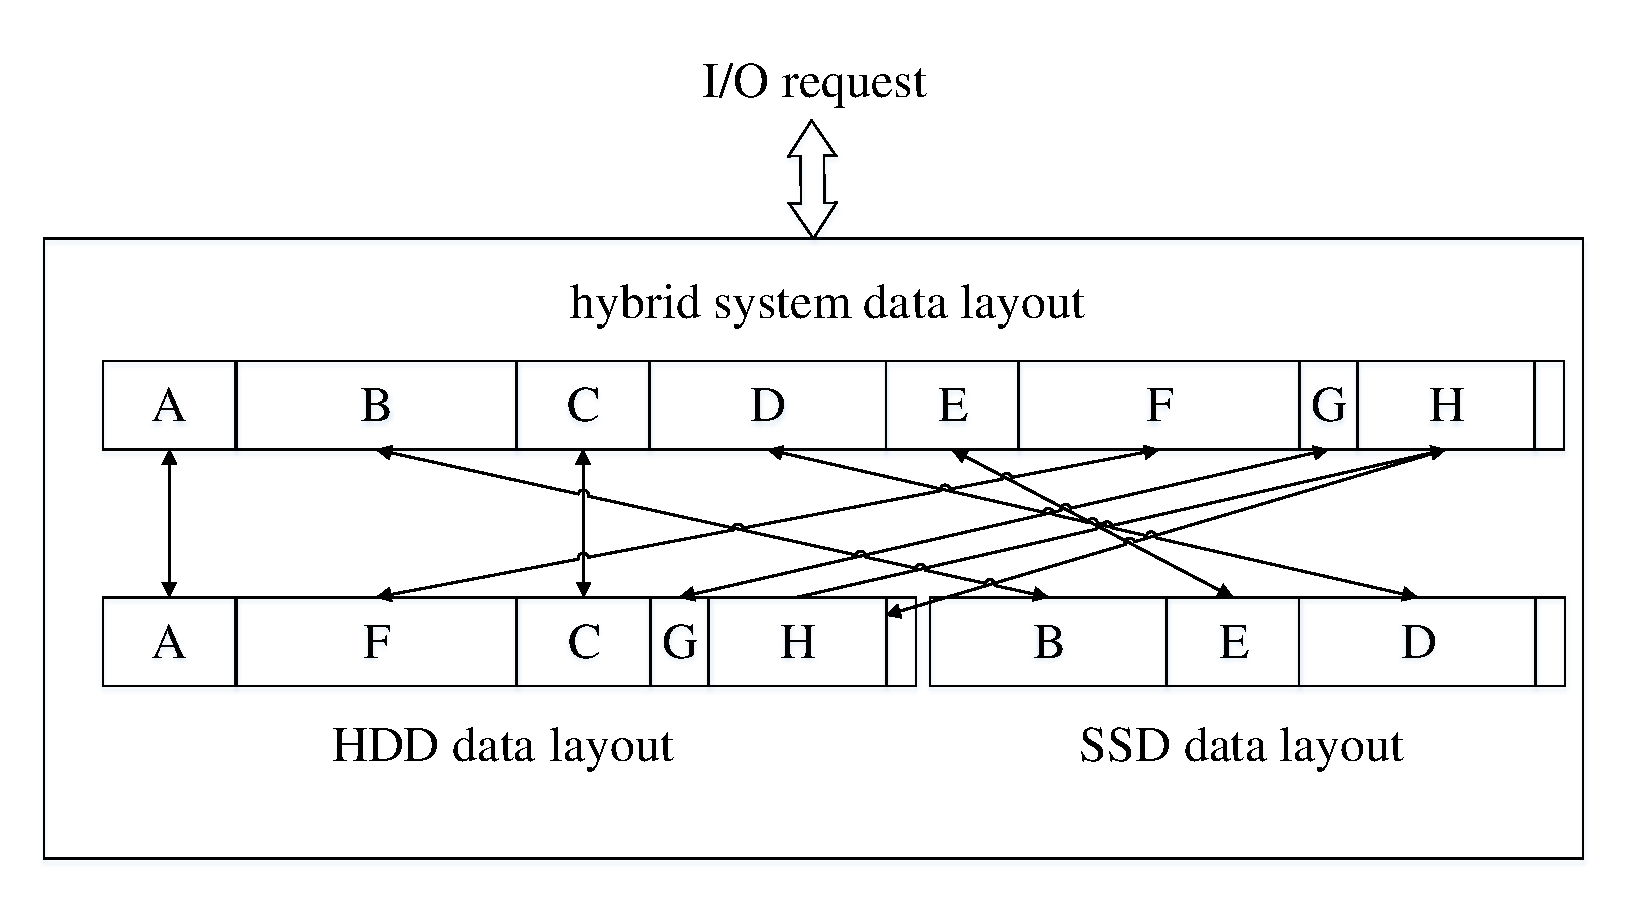
\includegraphics[width=0.8\textwidth]{single_layer_architecture.pdf}
    \bicaption[fig:single_layer_architecture]{同层混合存储系统架构}{同层混合存储系统架构}{Fig}{single-layer hybrid storage system architecture}
\end{figure}

\section{数据映射策略}

无论混合存储系统是分层架构还是同层架构,最后的数据都是以block为单位存放到实际设备上,因此对于每个block的I/O请求需要将其映射到具体的真实设备,这就需要考虑映射的粒度问题与映射的规则。

映射粒度是指在混合存储系统中系统能操作的数据的最小单位,它可以只是一个block的大小,也可以是多个block的大小,但应保证是block大小的整数倍。一般而言,映射粒度分为block级、文件级与Extent级三个级别。映射规则是指混合存储系统中的逻辑地址与实际设备的物理地址的转换规则。一般而言,映射规则分为纯计算类型、依靠映射表类型与计算和映射表混合类型三种。

\subsection{块级映射策略}

块级映射即以4KB的块(block)为操作数据的最小单位。所有的实际设备以4KB为大小划分为多个block,对混合存储系统中的每个block的I/O请求依照特定映射规则,映射到具体的实际设备进行实际操作。一般而言,块级映射策略用于分层架构的混合存储系统中,其映射规则与高速缓存和主存的映射规则类似,可分为全相联、直接映射和组相联三种。全相联即是指HDD的任一block可以映射到SSD的任一block,直接映射是指HDD的第j块block只能映射到满足如下特定关系的SSD的第i块block中(i=j \  mod \  SSD的block数)。组相联则是结合了全相联与直接映射,首先将多个block组成一个组,HDD的组与SDD的组之间采用直接映射的方式,而组内部的块则采用全相联的方式映射。

块级映射的映射策略较为简单,且可以以最细的粒度对数据进行操作,但是粒度越细,系统的额外开销也就越大。虽然HDD映射到SSD时可以通过直接映射的方式避免映射表,但是当需要将SSD的数据写回到HDD时势必需要一张映射表才能找到正确的位置。假设SSD的容量为100GB,映射表的每个block对应的表项的大小为20bytes,那么整个映射表的大小约为500MB,并且由于映射表是频繁访问的数据,需要驻留在内存中,因此最终整个系统需要500MB的额外内存开销,这对普通用户而言属于不可接受的额外开销大小。另外对于顺序读写请求,实际这些请求无论是全部放在SSD上进行或者都放在HDD上进行性能都相差不多,但块级映射可能会将顺序读写请求中的一些数据映射到SSD上另一些则映射到HDD上,最终导致顺序读写请求被分散到SSD和HDD上变成两个随机读写请求,这会极大影响性能。此外,在分层架构中,多个HDD的block会被映射到SSD的同一个block上,那么当发生碰撞时的替换策略对系统的性能影响也很大。

\subsection{文件级映射策略}

文件级映射即以文件为组织block的最小操作单位,同一个文件中的不同block会被映射到同一个设备上,同样,对数据的冷热识别、缓存的最小单位、数据迁移的最小单位也都是文件。相比块级映射,文件级映射的粒度显然粗很多,因此系统的额外开销会小很多,但是由于文件的大小不一,可能会存在很大的文件,当这些文件在分层架构中被缓存需要写回时或者在同层架构中需要被迁移时,系统的负载会一下子增高,而不像块级映射会比较平稳。

\subsection{Extent级映射策略}

Extent级映射即将多个block组成一个extent,以extent作为最小的操作单位,同一个extent中的block会被映射到同一个设备上。与文件级映射不同,同一个文件的block在物理存储上可能不连续,而Extent级映射则通常是将物理连续的多个block组成一个extent。extent的大小可以自由指定,这就让Extent级映射变得很灵活,但同时extent的大小十分讲究,如果设定的太小,那么系统的额外开销就会增加,同时也可能会有顺序读写性能下降的问题,而如果设定的太大,那么系统在冷热数据的识别上就会不精确,并且同样会在写回或者迁移上造成系统的负载瞬间增高。

\section{冷热数据识别策略}

冷热数据识别策略负责将数据区分为冷数据与热数据,提供将需要访问的数据放在高速设备上而将不经常访问的数据放在低速设备上的依据。冷热数据识别策略直接决定数据是否能被存在与其访问频度相符的设备上,因此冷热数据识别的准确性会直接影响系统的整体性能,冷热识别策略可大致分为块级冷热识别策略与文件/Extent级冷热识别策略,下面将分别介绍。

\subsection{块级冷热识别策略}

块级冷热识别策略是粒度最细的冷热识别策略,以块为冷热程度统计的最小单位。块级冷热识别策略将访问频率高的块标记为热数据,其他的标记为冷数据,由于SSD的写前擦除与擦除次数限制的特性,块级冷热识别策略在SSD的内部设计中经常有被应用以使SSD中不同块的负载均衡,使不同块的擦除次数保持平衡。

块级冷热识别策略的优势在于它真正识别出了哪些数据块是最热的数据。但是它只是给出了微观的最优解,但在宏观上未必是最优的。比如对于一组顺序读或顺序写请求,可能这组请求中涉及的数据块有的是冷数据有的是热数据,那么它们就会被存放在不同设备上,使得原本的顺序请求会被打散为在不同设备上的随机请求,这反而会降低系统的性能。

块级冷热识别的算法有很多,经典的有FIFO、LRU等算法,近年来也有ARC\cite{megiddo2003arc}、Clock-Pro\cite{jiang2005clock}、多哈希函数\cite{hsieh2006efficient}、多布隆过滤器\cite{park2011hot}、WDAC\cite{park2011hot}等算法。经典的FIFO、LRU算法虽然计算简单、实现简单,但是热点识别的准确率不高,比如当发生一个很长的循环遍历时,FIFO或者LRU的队列或者链表会被反复替换,导致系统的性能下降。ARC等新算法则通过使用新近性和频度来判断数据的冷热程度,虽然增加了额外的开销和提高了实现的复杂度,但是提高了热点识别的准确率,并且能够抵抗循环遍历造成的热点冲刷。

\subsection{文件/Extent级冷热识别策略}

文件/Extent级冷热识别策略以文件或者Extent为冷热程度统计的最小单位。每个块的I/O请求都会影响该块所属的文件或Extent的热度,同时除了文件或Extent中块的访问频率,该粒度下还可引入文件或Extent中热点块的分布、带宽等更宏观的指标来对更新文件或Extent的冷热程度。

文件/Extent级冷热识别策略的优势在于与块级冷热识别策略相比,更粗的粒度能带来更小的系统额外开销,并且可以同时从微观与宏观两个方面进行热点识别,能够识别出顺序读写请求与随机读写请求,以此为依据避免将顺序读写请求打散到不同设备上。

\section{数据写回/迁移策略}

在混合存储系统中最理想的情况是将热数据都存放在高速设备上,而将冷数据放在低速设备上,但由于数据的冷热程度会不断变化,并且高速设备的容量有限可能并不能存放所有热数据,因此会发生数据不处在与其冷热程度匹配的设备的情况,数据写回/迁移策略就是负责将数据迁移到与其冷热程度匹配的设备上,以提高系统整体的性能。数据写回/迁移策略需要考虑哪些数据需要写回/迁移、何时写回/迁移这些数据、在数据迁移中如何保证系统对外性能这三个问题。

写回/迁移数据的选择根据冷热识别策略决定,一旦冷热识别算法确定,通过该算法就能直接确定哪些热数据处在低速设备上,哪些冷数据处在高速设备上,针对这些数据再以对应的粒度:块级、文件级、Extent级生成待写回/迁移的数据集合即可。

数据的写回/迁移时机大致可分为静态与动态两种策略。静态策略是指系统周期性地对数据进行写回或迁移,静态策略一般选择在系统负载轻的时候(如半夜之后)进行大规模的写回/迁移,因此系统的性能波动对外影响较小,但是静态策略无法及时针对数据的冷热变化作出响应,无法实时达到系统的理论最大性能。动态策略是指不定期地对数据进行写回或迁移以对数据的冷热变化作出实时响应,动态策略可以保证系统的性能一直保持尽可能高,但是动态策略可能会让系统的性能波动变大,并且在系统重负载时影响到对外性能,尤其是当粒度为文件/Extent级时,甚至可能导致系统对外表现为不可用的状态。

\section{最优化存储设备组合}

最优化存储设备组合是指在保证系统达到性能需求的前提下尽可能降低系统的成本,这也是混合存储系统设计中要考虑的问题。该问题需要考虑系统架构、系统负载类型、存储设备的特性等诸多因素。该问题的解决可分为静态策略与动态策略两种。

\subsection{静态策略}

静态策略是指在构建混合存储系统的时候就选取好不同存储设备的型号、数量等,在混合存储系统上线运行后就不再变更,如果需要变更,则需要先将系统停止后更改配置再运行。目前静态策略的生成分为通过模拟\cite{guerra2011cost}给出最优解与通过理论推导计算\cite{kim2011hybridstore}给出最优解两种。

\subsection{动态策略}

动态策略是指在混合存储系统运行过程中能够不需要停止运行就能重新适应用户的新需求,比如在系统运行的过程中对存储设备的热插拔,在系统运行过程中冷热数据识别策略或者数据写回/迁移策略的动态变更等等。

\section{本章小结}

本章主要介绍了混合存储系统设计中的关键问题。首先介绍了系统架构,对分层架构和同层架构进行了阐述;然后介绍了数据映射策略,对块级、文件级、Extent级三种不同映射策略进行了简单的介绍与对比分析;之后介绍了冷热数据识别策略;然后介绍了数据写回/迁移策略,对静态与动态两种策略进行了简单的对比分析;最后介绍了最优化存储设备组合。
%# -*- coding: utf-8-unix -*-
%%==================================================
%% chapter01.tex for SJTU Master Thesis
%%==================================================

%\bibliographystyle{sjtu2}%[此处用于每章都生产参考文献]
\chapter{开源混合存储系统分析}
\label{chap:opensource_intro}

目前,开源的混合存储系统中被使用较为广泛的是flashcache、dm-cache、bcache这三个系统,但是对于这三个系统的研究主要集中在对他们的算法研究\cite{杨宗2013flashcache, 唐华敏2015bcache},而对他们的对比分析比较少。本章将首先对flashcache、dm-cache、bcache这三个开源混合存储系统分别从系统架构、数据映射策略、冷热数据识别算法、数据写回/迁移策略、最优化存储设备组合进行介绍,然后对他们从性能和特性两方面进行对比分析。

\section{flashcache}

\subsection{系统架构}

flashcache基于Device Mapper,采用分层架构,将缓存设备与后台设备统和为一块逻辑设备,缓存设备作为后台设备的数据缓存。

\subsection{数据映射策略}
\label{sec:flashcache_mapping}
flashcache采用块级映射策略中的组关联映射规则,通过set associative hash\cite{kimmel2014set}将缓存设备分成多个固定大小的set(一个set默认为512个block)并组织起来,将请求的block的起始扇区(dbn)通过公式\ref{eq:dbn_to_set}映射到target set,再在target set内部进行线性探测获取block,如图\ref{fig:flashcache_map}所示。

\begin{equation}
    \label{eq:dbn_to_set}
    target \ set = \frac{dbn}{block size \times set size} mod (set \  number)
\end{equation}

\begin{figure}[!htp]
    \centering
    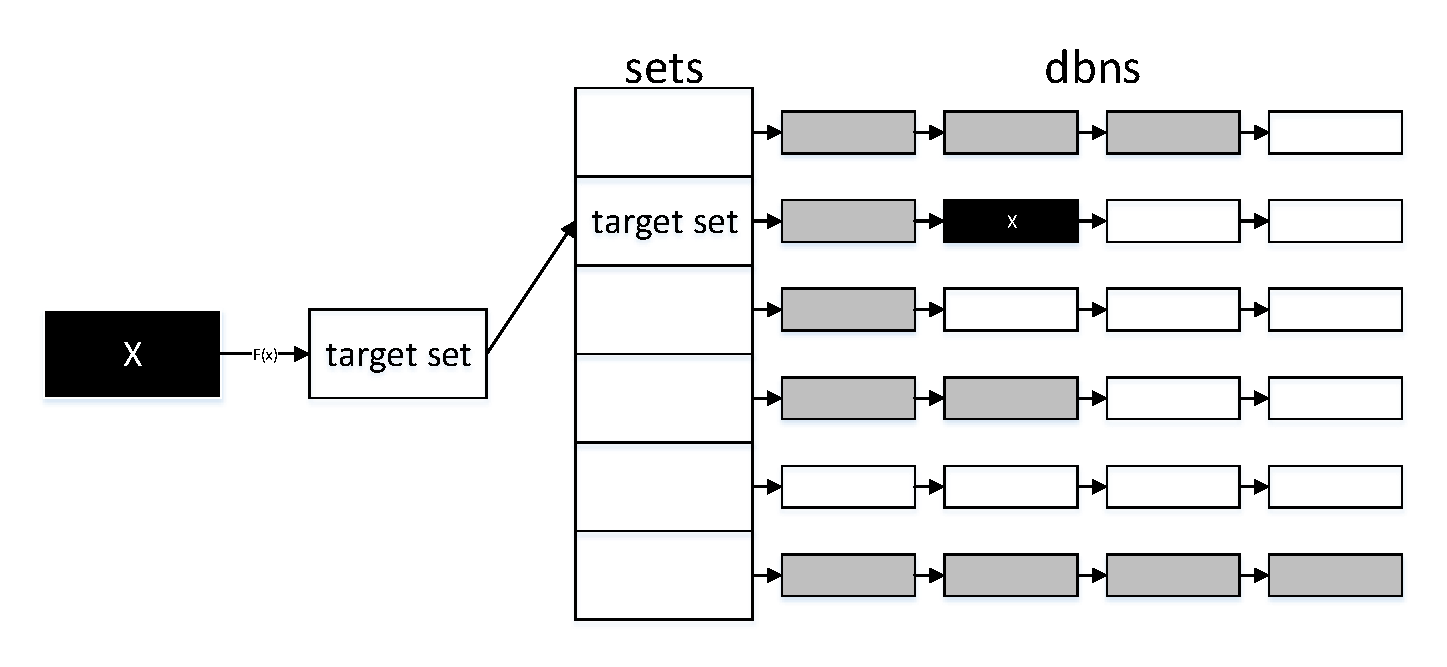
\includegraphics[width=0.8\textwidth]{flashcache_map.pdf}
    \bicaption[fig:flashcache_map]{flashcache的组相联映射}{flashcache的组相联映射}{Fig.}{group mapping in flashcache}
\end{figure}

\subsection{冷热数据识别算法}

flashcache以块级对数据进行冷热识别,采用双层lru链表结构将数据分为频繁访问的数据、偶尔访问的数据以及冷数据,如此一来,大量的遍历型I/O请求并不会导致大量的缓存失效,并且flashcache支持识别顺序性读写请求并略过对顺序性读写请求中数据的缓存操作。

\subsection{数据写回/迁移策略}

flashcache在每次I/O调用及每次I/O调用的回调时触发将脏数据从缓存设备写回到后台设备,并限制每次写回的脏数据的块数量,因此可以稳定地刷出脏数据而不会造成系统的负载突发性增长,另外可以设置将所有脏数据强制全部写回。

\subsection{最优化存储设备组合}

flashcache采用静态策略,并且限制在创建混合存储系统时,缓存设备与后台设备都只能有一个。

\section{dm-cache}

\subsection{系统架构}

dm-cache基于Device Mapper,并且已进入Linux内核主线,因此与Linux内核的Device Mapper结合更加紧密,dm-cache中许多函数的实现直接依赖于对Device Mapper相关库中的函数的调用。

\subsection{数据映射策略}

dm-cache采用Extent级映射策略,将缓存设备分成大小固定的缓存块(缓存块大小为32KB的整数倍),缓存块通过hash表组织避免了set associative hash的利用率低和冲突问题。

\subsection{冷热数据识别算法}

dm-cache最初使用multi queue对冷热数据进行管理与识别,最新的则是对multi queue进行优化,使用smq(stochastic multi queue,随机多队列模式)对缓存块进行管理。smq本质就是一个多层lru算法,最多可以有64层,层数代表数据的冷热程度不同。smq并不记录缓存块的命中数,并根据命中数记录在不同层,因为这样会导致命中数越是高的层记录的缓存块越少而命中数越少的层记录的缓存块越多,最终导致层与层之间不平衡。smq在缓存块命中时将该缓存块与它上层中最近最少使用的缓存块进行交换,达到不同层平衡的效果。

\subsection{数据写回/迁移策略}

dm-cache在每次I/O调用时触发将脏数据从缓存设备写回到后台设备,并限制通过阈值限制每秒写回的脏数据块数。

\subsection{最优化存储设备组合}

dm-cache采用静态策略,并且限制在创建混合存储系统时,缓存设备与后台设备都只能有一个。

\section{bcache}

\subsection{系统架构}

bcache没有采用Device Mapper而是自己实现了一套系统,采用分层架构,将缓存设备与后台设备统和为一块逻辑设备,缓存设备作为后台设备的数据缓存。

\subsection{数据映射策略}

bcache采用Extent级映射策略,将缓存设备分成大小固定的bucket(默认512KB),bucket内部空间采用追加分配的方式,记录当前的偏移量,下次分配时从当前偏移量继续向后分配,数据映射到bucket时主要有2个考量:优先将连续的数据映射到同一个bucket中即使他们可能来源于不同进程的I/O操作;优先将同一进程操作的数据映射到同一bucket中。bucket通过B+树进行管理,每个树节点内部为4个bset结构,每个bset存有排好序的bkey。

\subsection{冷热数据识别算法}

bcache在每个bucket中记录16位长的优先级,每次bucket命中,优先级加一,同时所有bucket的优先级周期性减少,bcache通过bucket的优先级实现lru算法进行冷热数据的识别。

\subsection{数据写回/迁移策略}

bcache当bucket使用超过阈值时会触发垃圾回收,或者当用作缓存的缓存设备容量不够时直接集中写回到后台设备,这一操作会耗费大量CPU(遍历btree)和触发大量后台设备I/O操作。

\subsection{最优化存储设备组合}

bcache采用动态策略,bcache并不是通过单条语句创建相应的bcache设备,而是分为添加缓存设备与添加后台设备的语句,当添加后台设备后自动出现相应的bcache设备,之后仍可以通过相应命令动态增加设备。目前bcache对于动态增加后台设备有比较好的支持,但对于动态增加缓存设备还处于初步阶段。

\section{对比分析}

flashcache、dm-cache、bcache经过测试后的特性对比如下所示。

\subsection{可靠性}

flashcache的可靠性较高,采用分散式刷脏数据策略(控制刷脏数据速率),所以在I/O重负载的情况下系统不会表现为无法响应的状态,表现优秀。当作为缓存的SSD满后,且数据没有重叠时会击穿缓存,直接访问磁盘。 

dm-cache的可靠性较弱,在I/O重负载的情况下系统会因为刷脏数据无法响应,但是因为刷脏数据的效率较高,所以未响应表现为间歇性。当作为缓存的SSD满后,且数据没有重叠时会击穿缓存,直接访问磁盘。 

bcache的可靠性弱,在I/O重负载的情况下系统会长时间无法响应,因为是按bkey遍历树刷出,刷脏数据比较慢,所以系统未响应时间很久,不可控。当作为缓存的SSD满后,且数据没有重叠时会击穿缓存,直接访问磁盘。

\subsection{被缓存的数据大小}

flashcache严格按照缓存块大小进行缓存,不符合条件即大小不一致或边界未对齐的读写请求都不会进行缓存。

dm-cache缓存块采用固定大小,但是当小于设置的缓存块大小时也会被缓存,模块会先从后台设备上把数据迁移到作为缓存设备中,然后进行I/O操作。 

bcache可以缓存任意大小的数据。用bkey追踪,放入树中,因此可能会产生大量的小块。

\subsection{内存开销}

flashcache每个缓存块占用25字节空间,假设被用作缓存的SSD大小为20GB,当缓存块大小设置为4KB时,内存占用约为110MB,在缓存块大小同样的情况下,内存占用和用作缓存的SSD的容量大小基本成正比。  

dm-cache每个缓存块占用24字节空间,假设被用作缓存的SSD大小为20GB,当缓存块大小设置为4KB时,内存占用约为105MB,在缓存块大小同样的情况下,内存占用和用作缓存的SSD的容量大小基本成正比。

bcache占用的内存大小难以直接估计,与用来存元数据的bucket的数量相关,当缓存设备容量较大的时候,这个值会很大(假设缓存大小为26GB,块大小设置为4KB,则大概占用600MB的内存)。树动态增长,树节点数只增不减,当内存不足时,会触发回收,但是查看节点状态时,会把所有数据读取到内存中。大概的内存消耗是80个树节点消耗20MB,节点个数和缓存设备的容量大小正相关。

\subsection{拔盘测试}

flashcache在有I/O负载的情况下,突然拔出作为缓存的SSD,用作测试的fio程序卡顿30秒后返回,kcopyd高负载调用几分钟后恢复正常,但是磁盘无法访问; 如果拔出磁盘,fio卡顿1分钟左右返回,但是 kcopyd一直报错,且等待1小时也未恢复正常。   

dm-cache在有I/O负载的情况下,突然拔出作为缓存的SSD,用作测试的fio程序卡顿30秒后返回,kcopyd高负载调用几分钟后恢复正常,但是磁盘无法访问; 如果拔出磁盘,fio卡顿1分钟左右返回,但是 kcopyd一直报错,且等待1小时也未恢复正常。 

bcache在有I/O负载的情况下,拔除SSD会导致系统高负载卡死,这是由于对树节点遍历操作会一直出错,并且会一直重试。 

\subsection{断电测试}

flashcache在有脏数据情况下,突然重启系统(强行物理关机),重启后恢复flashcache,脏数据可以继续刷出。

dm-cache在有脏数据情况下,突然重启系统(强行物理关机),重启后恢复dm-cache,脏数据可以继续刷出。 

bcache在有脏数据情况下,突然重启系统(强行物理关机),重启后恢复bcache,脏数据可以继续刷出。

\subsection{性能测试}
      
对flashcache、dm-cache、bcache的读写性能的测试对比,测试前预先进行了数据预热使缓存数据接近100\%以测试系统的最大性能。测试工具使用fio,分别测试I/O块设置为4K、32K下混合存储设备使用裸盘、XFS文件系统下系统的随机读写性能。 

测试环境如表\ref{tab:test_environment}所示

\begin{table}[H]
    \zihao{5}
    \centering
    \bicaption[tab:test_environment]{flashcache、dm-cache、bcache读写性能测试环境}{flashcache、dm-cache、bcache读写性能测试环境}{Table}{test environment of flashcache, dm-cache and bcache}
    \begin{tabular}{cc} \toprule
      机器类型 & 普通台式机 \\ \midrule
      CPU & 单核AMD CPU\\
      内存 & 1GB DDR3\\
      SSD & 120GB intel350 \\
      HDD & WD 1TB 7200rpm绿盘\\
      \bottomrule
    \end{tabular}
\end{table}

表\ref{tab:standard_test}为对被用作缓存设备的SSD进行的基准测试,以与后续测试进行对比,可以发现当使用XFS文件系统时性能有所下降,这是由于文件系统相比裸盘多了元数据的修改操作。

\begin{table}[H]
    \zihao{5}
    \centering
    \bicaption[tab:standard_test]{基准测试}{基准测试}{Table}{standard test}
    \begin{tabular}{cccc} 
      \toprule
      I/O类型 & 随机读IOPS & 随机写IOPS & 混合随机读写(r/w) \\ 
      \midrule
      I/O块4KB,裸盘 & 34.6k & 25.4k & 8746/8743 \\
      I/O块4KB,XFS & 38.2k & 15.2k & 7400/7414 \\
      I/O块32KB,裸盘 & 5310 & 3840 & 1498/1505 \\
      I/O块32KB,XFS & 6385 & 3831 & 1505/1513 \\
      \bottomrule
    \end{tabular}
\end{table}

表\ref{tab:flashcache_test}为使用flashcache的测试,由于flashcache只严格缓存缓存块大小边界对齐的数据,由于XFS文件系统默认块大小为4K,大于这个大小的IO文件系统的边界和块设备的边界未必对齐,所以在flashcache中不会被缓存,因此缓存块32k IO块32K XFS条件下的性能接近磁盘的性能。 

\begin{table}[H]
    \zihao{5}
    \centering
    \bicaption[tab:flashcache_test]{flashcache测试}{flashcache测试}{Table}{flashcache test}
    \begin{tabular}{cccc} 
      \toprule
      I/O类型 & 随机读IOPS & 随机写IOPS & 混合随机读写(r/w) \\ 
      \midrule
      缓存块4KB,I/O块4KB,裸盘 & 22.3k & 10.2k & 5725/5741 \\
      缓存块4KB,I/O块4KB,XFS & 23.5k & 14.6k & 6392/6409 \\
      缓存块32KB,I/O块32KB,裸盘 & 4227 & 2250 & 1717/1721 \\
      缓存块32KB,I/O块32KB,XFS & 200-300 & 200-300 & / \\
      \bottomrule
    \end{tabular}
\end{table}

表\ref{tab:dm-cache_test}为使用dm-cache的测试。dm-cache的缓存块大小范围设置为32KB-1GB,可以发现dm-cache框架下使用XFS文件系统比使用裸盘的性能高,这是由于dm-cache采用了smq算法,而XFS文件系统的数据组织结构导致了这一结果。 

\begin{table}[H]
    \zihao{5}
    \centering
    \bicaption[tab:dm-cache_test]{dm-cache测试}{dm-cache测试}{Table}{dm-cache test}
    \begin{tabular}{cccc} 
      \toprule
      I/O类型 & 随机读IOPS & 随机写IOPS & 混合随机读写(r/w) \\ 
      \midrule
      缓存块32KB,I/O块4KB,裸盘 & 11.3k & 700-1200 & 6787/6878 \\
      缓存块32KB,I/O块4KB,XFS & 17.2k & 11.9k & 4777/4850 \\
      缓存块32KB,I/O块32KB,裸盘 & 4260 & 3009 & 671/673 \\
      缓存块32KB,I/O块32KB,XFS & 4055 & 3032 & 1467/1471 \\
      \bottomrule
    \end{tabular}
\end{table}

表\ref{tab:bcache_test}为使用bcache的测试。由于bcache没有缓存块的概念,可以缓存任意长度的I/O对象,因此在小IO时表现优异。

\begin{table}[H]
    \zihao{5}
    \centering
    \bicaption[tab:bcache_test]{bcache测试}{bcache测试}{Table}{bcache test}
    \begin{tabular}{cccc} 
      \toprule
      I/O类型 & 随机读IOPS & 随机写IOPS & 混合随机读写(r/w) \\ 
      \midrule
      I/O块4KB,裸盘 & 25.4k & 21.6k & 9589/9615 \\
      I/O块4KB,XFS & 23.5k & 20.9k & 967/972 \\
      I/O块32KB,裸盘 & 3069 & 1746 & 967/972 \\
      I/O块32KB,XFS & 2660 & 1622 & 590/591 \\
      \bottomrule
    \end{tabular}
\end{table}

基准测试、flashcache、dm-cache、bcache的随机读性能对比图如图\ref{fig:opensource_randread}所示。可以看到flashcache和bcache的性能比较接近而dm-cache在小I/O块的时候性能不如flashcache和bcache,这是由于dm-cache的缓存块大小最小为32K,在小I/O块下,需要先从磁盘上提升数据再进行I/O操作。总的来看,在小I/O块时flashcache、dm-cache和bcache的性能都无法达到SSD的性能,而在大I/O块时则基本都接近SSD的性能。

\begin{figure}[H]
    \centering
    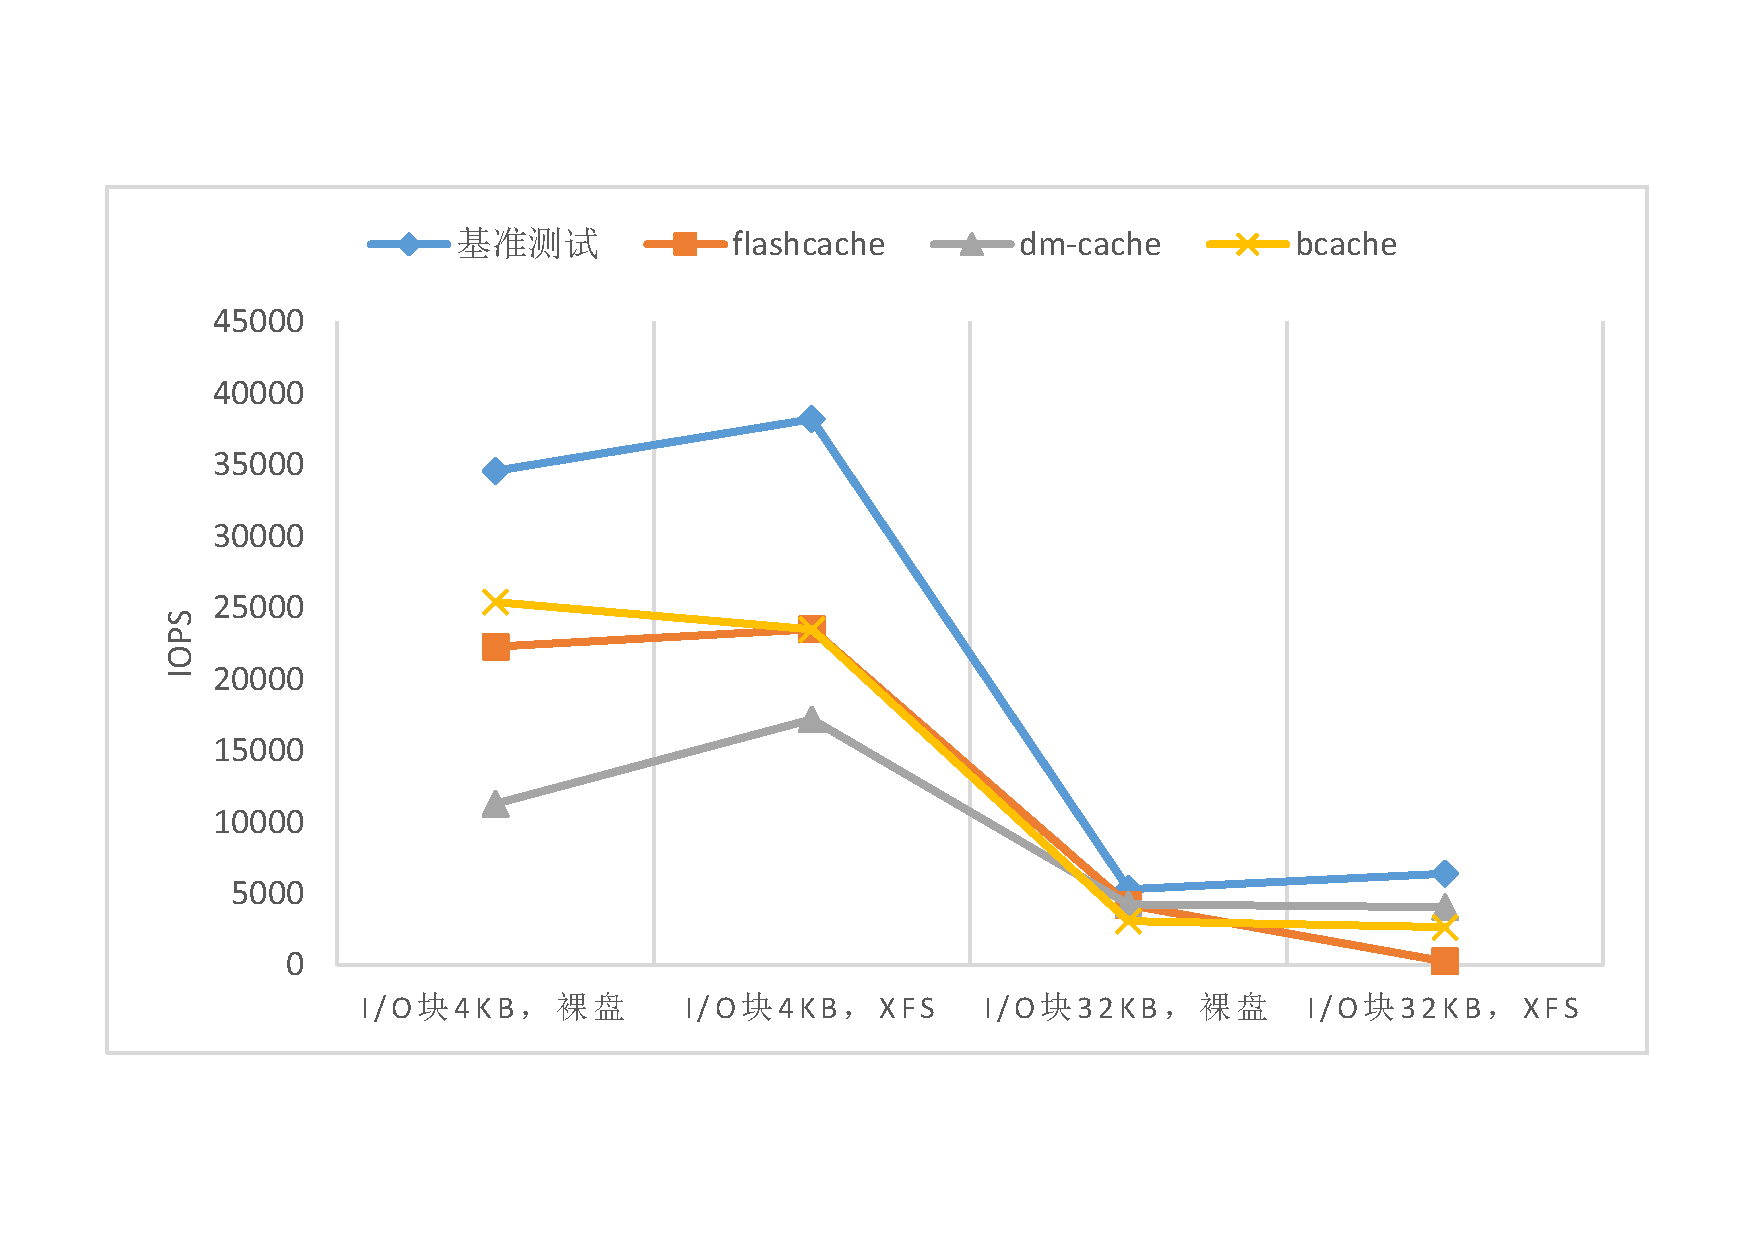
\includegraphics[width=0.7\textwidth]{opensource_randread.pdf}
    \bicaption[fig:opensource_randread]{基准测试、flashcache、dm-cache、bcache随机读性能对比}{基准测试、flashcache、dm-cache、bcache随机读性能对比}{Fig.}{comparison of random read among standard, flashcache, dm-cache and bcache}
\end{figure}

随机写性能对比图如图\ref{fig:opensource_randwrite}所示。可以看到相比随机读性能,flashcache、dm-cache和bcache三者的差距在小I/O时拉的更开,而在大I/O块时同样性能比较接近。与随机读不同,在随机写时,bcache的性能总体与SSD的性能持平,这是由于bcache采用日志追加的方式进行写操作处理,因此在小I/O块时性能非常优异。

\begin{figure}[H]
    \centering
    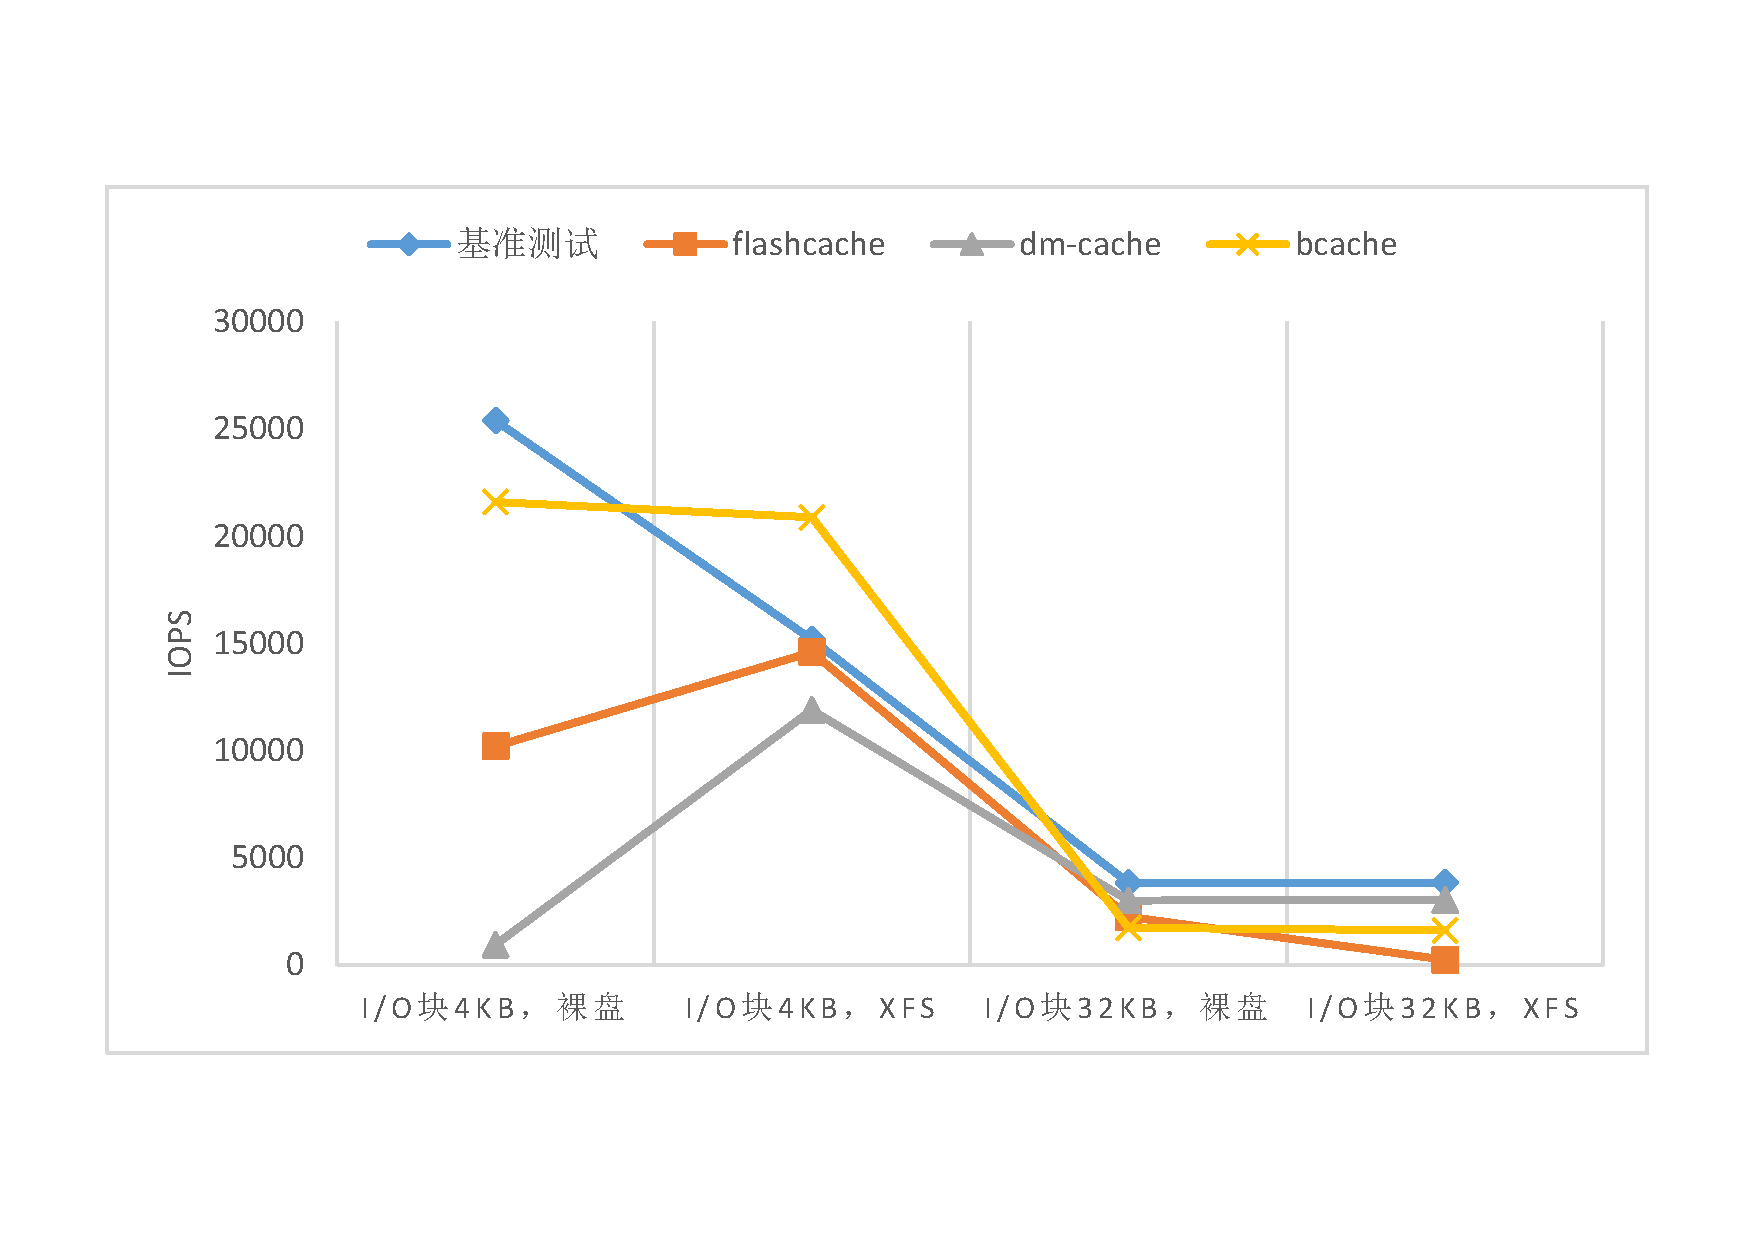
\includegraphics[width=0.7\textwidth]{opensource_randwrite.pdf}
    \bicaption[fig:opensource_randwrite]{基准测试、flashcache、dm-cache、bcache随机写性能对比}{基准测试、flashcache、dm-cache、bcache随机写性能对比}{Fig.}{comparison of random write among standard, flashcache, dm-cache and bcache}
\end{figure}

混合随机读写性能对比图如图\ref{fig:opensource_randrw_read}和图\ref{fig:opensource_randrw_write}所示。可以看到总体趋势仍然是在小I/O块时flashcache、dm-cache、bcache的性能差距会比较大,在大I/O块时性能则都很接近。并且总的来看,混合随机读写下,读性能与写性能几乎一样。与单纯的随机读或随机写性能差距较大的是bcache,在混合随机读写下bcache在小I/O块且使用XFS文件系统时性能有极具衰减。

\begin{figure}[H]
    \centering
    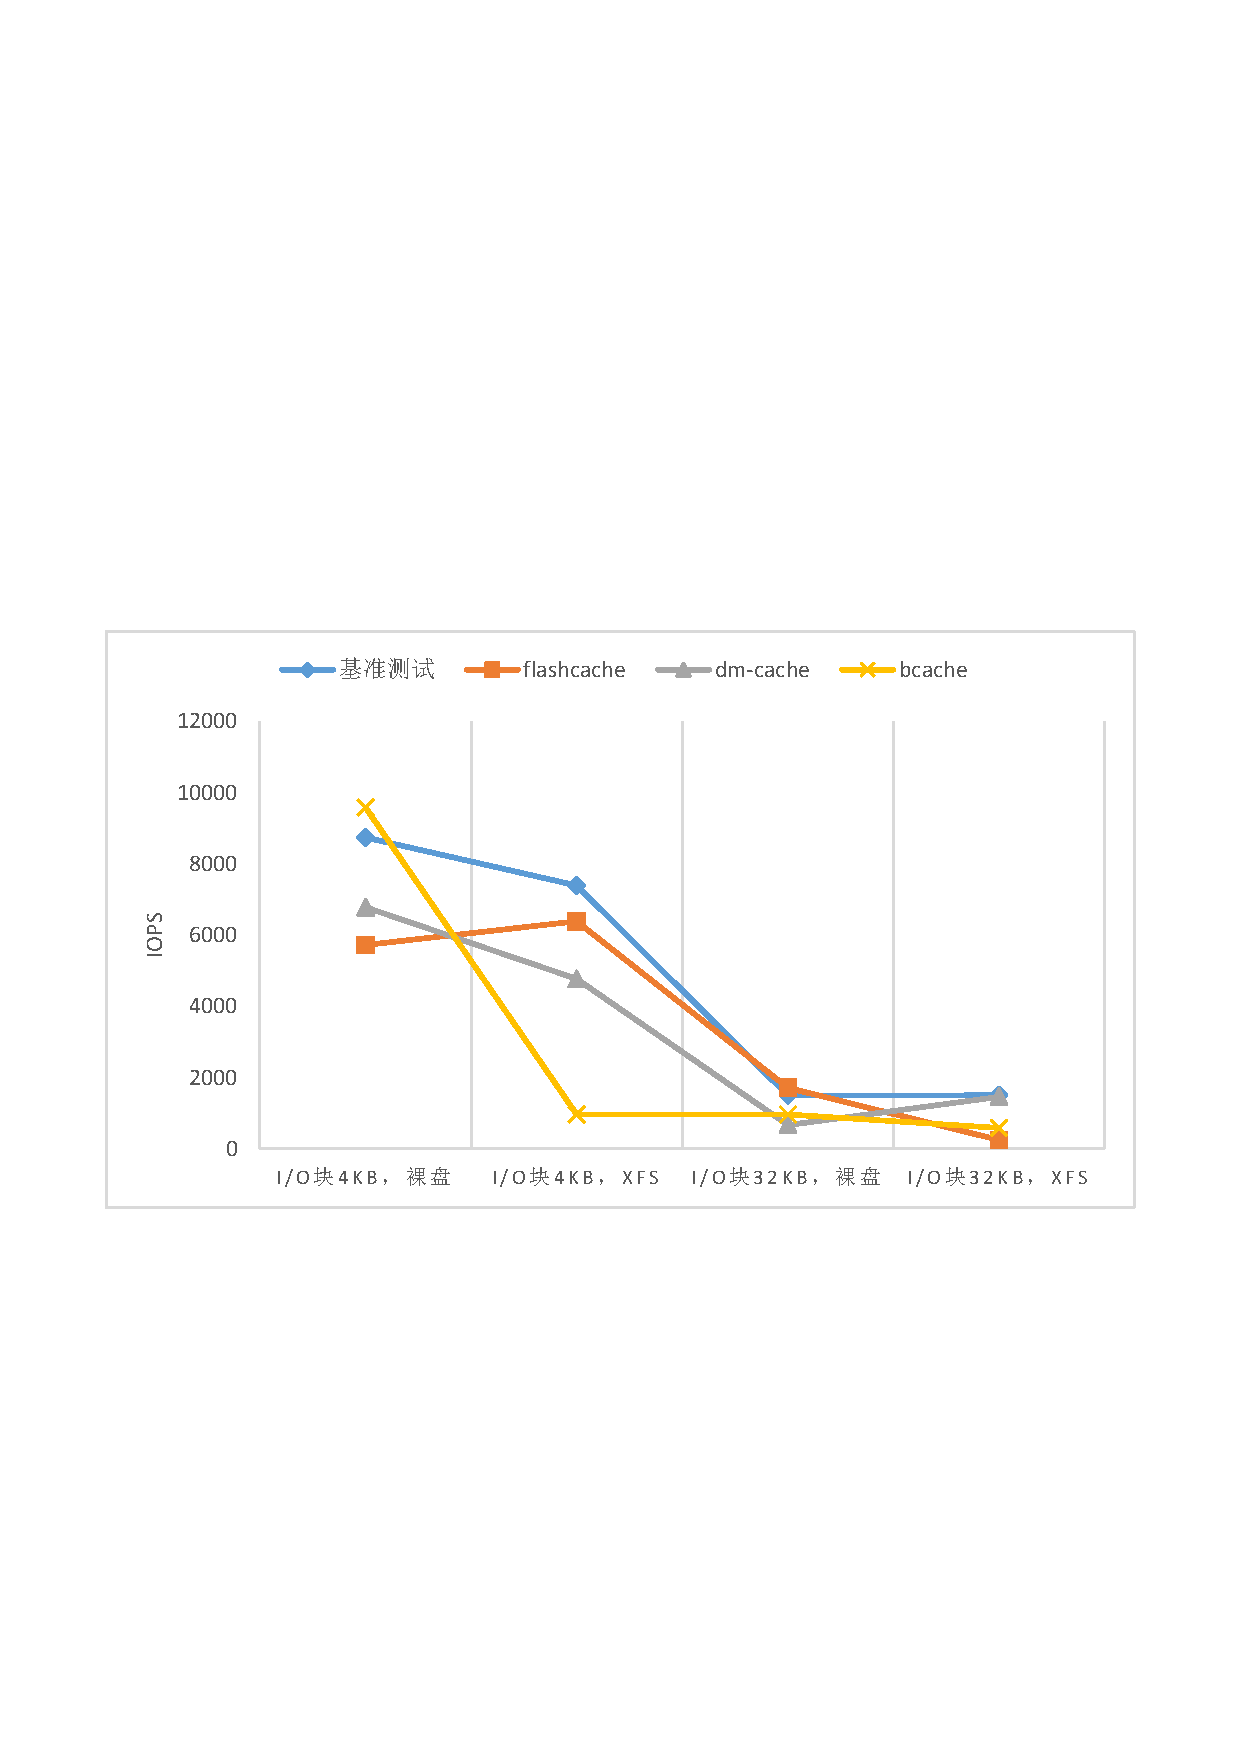
\includegraphics[width=0.7\textwidth]{opensource_randrw_read.pdf}
    \bicaption[fig:opensource_randrw_read]{基准测试、flashcache、dm-cache、bcache混合随机读写中读性能对比}{基准测试、flashcache、dm-cache、bcache混合随机读写中读性能对比}{Fig.}{comparison of random read/write read among standard, flashcache, dm-cache and bcache}
\end{figure}

\begin{figure}[H]
    \centering
    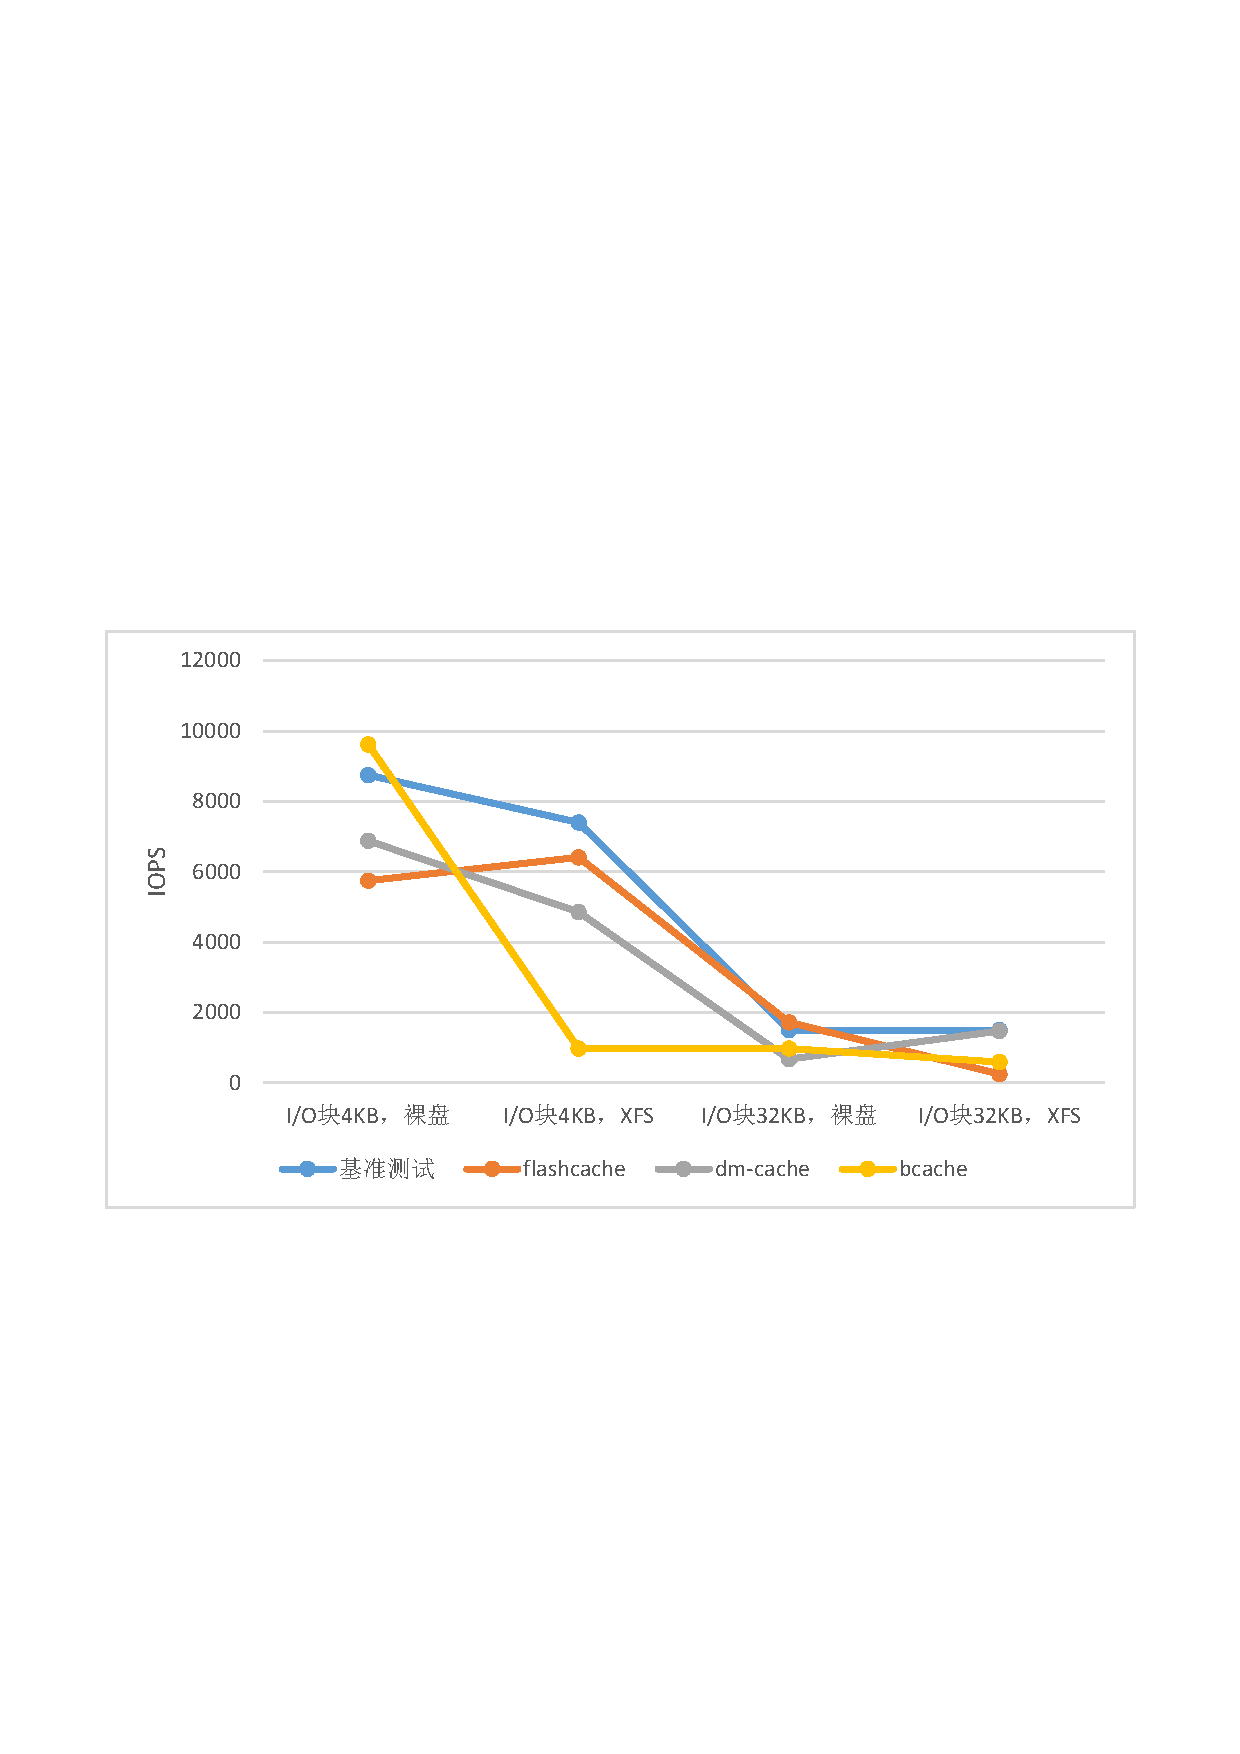
\includegraphics[width=0.7\textwidth]{opensource_randrw_write.pdf}
    \bicaption[fig:opensource_randrw_write]{基准测试、flashcache、dm-cache、bcache混合随机读写中写性能对比}{基准测试、flashcache、dm-cache、bcache混合随机读写中写性能对比}{Fig.}{comparison of random read/write write among standard, flashcache, dm-cache and bcache}
\end{figure}

\section{本章小结}

本章从上章提到的混合存储系统设计中系统架构、数据映射策略、冷热数据识别算法、数据写回/迁移策略、最优化存储设备组合这五个方面对现有三个开源混合存储系统flashcache、dm-cache、bcache进行了分析,并且经过测试给出了flashcache、dm-cache、bcache的特性对比以及性能对比。从特性对比来看flashcache在可靠性方面优于另两者,bcache在内存消耗方面有较大不足。从性能测试来看flashcache的缓存要求非常严格,必须设备边界对齐且长度一致才能被缓存,dm-cache和bcache则没这个限制。在I/O块4k时bcache表现优异,但是在大I/O块时表现不如flashcache和dm-cache。当缓存命中率接近100\%时,flashcache性能要略优于dm-cache。
%# -*- coding: utf-8-unix -*-
%%==================================================
%% chapter01.tex for SJTU Master Thesis
%%==================================================

%\bibliographystyle{sjtu2}%[此处用于每章都生产参考文献]
\chapter{系统设计}
\label{chap:sys_design}

本章首先介绍基于SSD、HDD的混合存储系统的设计动机与设计目标,然后展开描述了系统架构、数据映射策略、冷热数据识别策略、数据写回/迁移策略、最优化存储设备组合等设计。

\section{设计动机与设计目标}

\subsection{设计动机}

在上一章介绍了现在被广泛应用的三种开源混合存储系统flashcache、dm-cache和bcache,他们在性能、可靠性、内存开销等方面都有各自的优点与缺点,但有两个问题是这三个混合存储系统都未解决的。

第一个问题是这三个混合存储系统的最优化存储设备组合,他们都不支持将多存储设备与多后台设备统一为一个逻辑设备供用户使用。flashcache和dm-cache都仅支持单缓存设备对单后台设备,bcache支持单存储设备对多后台设备。对于普通用户而言,单个缓存设备已经足够应付正常的I/O负载,但对服务器级别的I/O负载来说,由于本身存储的数据量大,且I/O负载重,为了保证缓存的高命中率,缓存设备的容量也应相对数据量进行提升,但是如果混合存储系统仅支持单缓存设备,那么就需要单个大容量的缓存设备,成本会急剧上升,而如果混合存储系统支持多缓存设备,就可以以多个小容量的缓存设备实现大缓存容量,降低成本。

另一个问题是这三个混合存储系统都不支持针对不同进程设置不同权限,按权限分配进程的I/O带宽,由于系统整体的I/O带宽有限,在重负载情况下系统可能无法满足全部进程的I/O带宽要求,如果系统只是简单地将总I/O带宽平均分配给所有进程或者以先来先得的策略分配,可能会造成高权限的进程不如低权限进程的情况。为了解决这两个问题,需要设计一套新型混合存储系统,在保证系统的大容量、低成本、高性能的前提下实现对多缓存设备对多后台设备的支持以及对支持按进程权限分配I/O带宽的功能。

\subsection{设计目标}

本混合存储系统的设计目标如下:

\begin{enumerate}
    \item 大容量。系统应具有较大的容量,且应能支持多缓存设备对多后台设备的缓存。
    \item 低成本。系统的存储成本应接近HDD的存储设备。
    \item 高顺序读写性能。系统的顺序读写性能应至少接近HDD的性能。
    \item 高随机读写性能。系统的随机读写性能应接近SSD的性能。
    \item 支持I/O带宽按权限分配。系统应支持按照进程的权限分配不同进程的I/O带宽。

\end{enumerate}

\section{系统架构}

系统总体架构如图\ref{fig:system_architecture}所示。系统首先将缓存设备与后台设备各自虚拟成一个统一的存储空间的虚拟缓存设备和虚拟后台设备进行管理,然后将虚拟缓存设备与虚拟后台设备虚拟为一个设备设备进行统一管理,并提供给用户使用。系统在接收到I/O请求后,通过映射机制将I/O进行分割,然后将分割后的I/O交给缓存管理模块,缓存管理模块首先进行存储地址查找,如果在缓存设备上则直接返回地址,否则进入数据冷热识别,并经缓存替换策略后发起缓存数据的更新操作。虚拟缓存设备和虚拟后台设备在收到请求后也经过存储位置查找,将对数据块的请求交给对应的真实设备处理。

\begin{figure}[!htp]
    \centering
    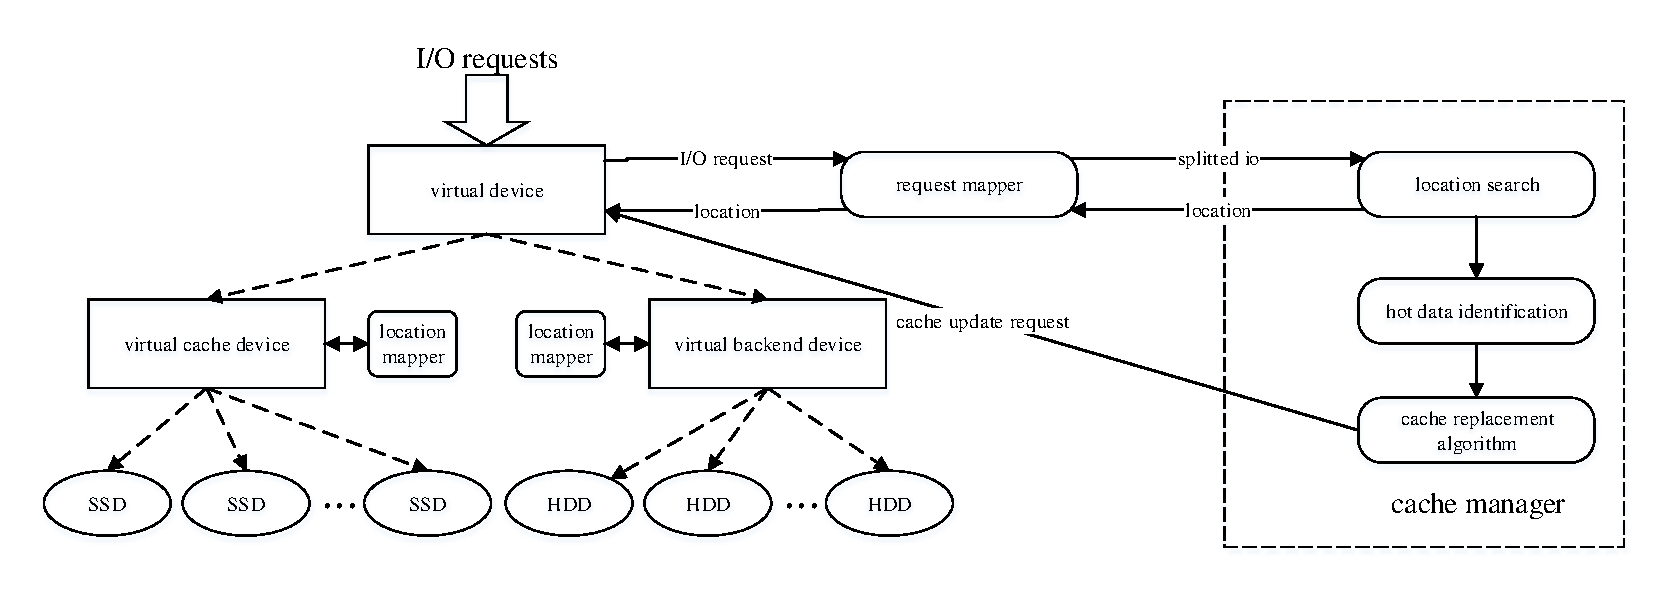
\includegraphics[width=\textwidth]{system_architecture.pdf}
    \bicaption[fig:system_architecture]{系统整体架构}{系统整体架构}{Fig}{overall system architecture}
\end{figure}

系统整体采用分层架构,利用SSD较高的随机读写性能将SSD用作随机I/O缓存,将HDD作为源存储介质存储所有的数据,SSD上存储HDD中数据的子集,系统可用容量等于HDD的总容量。数据的流动规则如图\ref{fig:data_flow}所示,系统将随机I/O请求交由SSD处理,将随机I/O请求交由HDD处理,SSD与HDD之间进行数据的交换,HDD将热数据写入到SSD中提高系统整体的性能,SSD将被替换的数据写回到HDD中保证系统的一致性。

\begin{figure}[!htp]
    \centering
    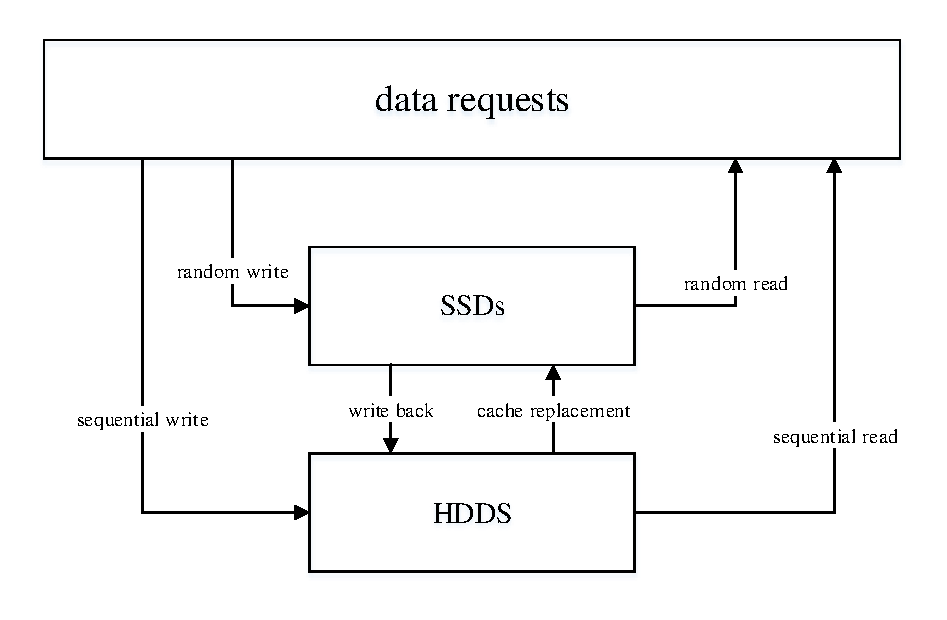
\includegraphics[width=0.8\textwidth]{data_flow.pdf}
    \bicaption[fig:data_flow]{数据流示意图}{数据流示意图}{Fig}{data flow}
\end{figure}

\section{数据映射策略}
TODO,与flashcache相同。

\section{冷热数据识别策略}

TODO,与flashcache相同。

\section{数据写回/迁移策略}

TODO,与flashcache相同。

\section{最优化存储设备组合}

在系统架构中可以看到,本系统对于多缓存设备和多后台设备的管理采用增加一层虚拟层的策略。系统不直接将多个缓存设备和多个后台设备统一为一个虚拟设备进行管理以供用户使用,而是首先将多个缓存设备统一成一个虚拟缓存设备,将多个后台设备统一成一个虚拟后台设备。

分层管理通过增加中间层,相比直接管理多个设备,系统可以将设备管理策略与系统架构、数据映射策略、冷热数据识别策略、数据写回/迁移策略等缓存策略隔离开,使策略的配置更简单。例如,如果要保证多个缓存设备的容量被均衡地使用,在直接管理下,相应的数据映射策略和数据写回/迁移策略都要对应修改,但在分层管理下,数据映射策略和数据写回/迁移策略可以维持不变,只需要改变设备管理策略,将多个设备以raid0生成对应虚拟设备即可。如果要保证数据的可靠性,配置多副本,则在直接管理下,需要将设备分组管理、分组操作,对应的各种操作都需要改变,而在分层管理下只需要以raid1配置设备即可。

分层管理虽然在策略配置上更灵活,但相比直接管理,系统在扩容上会略显不足。在直接管理下,对系统的扩容可以实现热扩容,即在系统运行的状态直接进行扩容操作,直接增加被管理的设备并更新对应的参数变化即可。与之相对,在分层管理下,由于设备管理与其它部分隔离,为了保证扩容后系统的正确性,需要先将虚拟缓存设备的数据全部写回虚拟后台设备,然后禁用缓存,对系统进行扩容,再开启缓存,系统整体会有性能下降的一段时间,且影响时间与被缓存的数据量有关,即约与虚拟缓存设备的容量成正比。

本文的研究认为,对于普通用户而言,系统基本不存在扩容这一行为,而对于服务器级用户而言,扩容也并不是一种经常进行的行为,但是对于设备管理策略的变更的频率确是相对而言比较高的。设备管理的策略主要与系统的I/O负载类型有关,变化比较多样,有的可能只是要求设备负载均衡,有的可能只是要求能提供灾备,但有的可能会很复杂,是多种简单策略的组合。如果采用直接管理的模式,虽然也能实现各种策略,但是对应的代码修改量会十分巨大,分层管理则可利用现有的技术如逻辑盘卷管理(LVM, Logical Volume Manager)\cite{wada2009logical}完成。

\section{I/O带宽按权限分配}

系统通过对不同进程按照各自权限分配IOPS来限制不同进程的I/O带宽,采用CFQ(Completely Fair Queuing)策略,如图\ref{fig:system_io_scheduler}所示,每个进程都被分配一个队列,每个I/O请求被放到对应进程的队列中,根据每个进程的权限不同,给每个进程的I/O请求分配不同的时间片数量,每个时间片取出I/O请求通过映射到实际设备进行请求处理。

\begin{figure}[!htp]
    \centering
    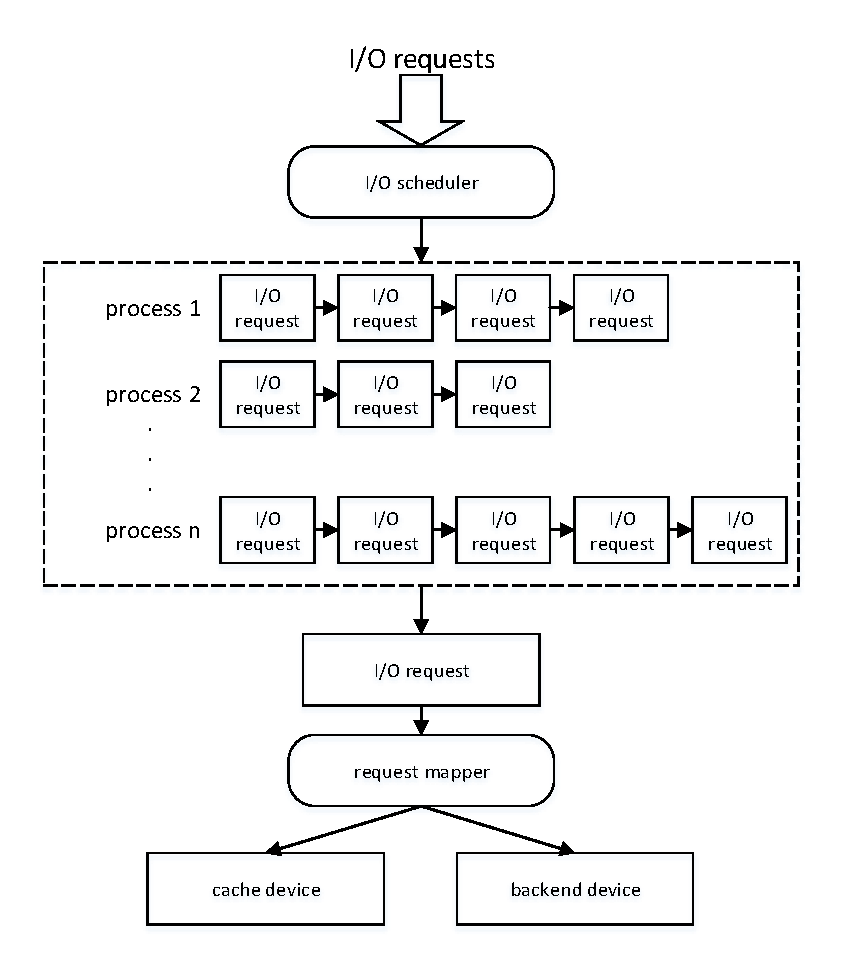
\includegraphics[width=0.8\textwidth]{system_io_scheduler.pdf}
    \bicaption[fig:system_io_scheduler]{I/O带宽分配流程}{I/O带宽分配流程}{Fig}{I/O bandwidth quota process}
\end{figure}

\section{本章小结}

本章介绍了系统在设计过程中所遇到的问题以及对分析与解决思路。介绍了系统的设计动机与设计目的,并对优化存储设备组合与I/O带宽按权限分配等问题的策略选择进行了分析,为接下来的系统实现做准备。
%# -*- coding: utf-8-unix -*-
%%==================================================
%% chapter01.tex for SJTU Master Thesis
%%==================================================

%\bibliographystyle{sjtu2}%[此处用于每章都生产参考文献]
\chapter{系统实现}
\label{chap:sys_implement}

上一章介绍了qscache系统的设计,这一章将首先介绍qscache系统实现所需的预备知识,进而介绍qscache系统的具体实现。

\section{预备知识}

由于qscache系统位于linux内核态,因此需要对内核中与系统实现相关的基本知识进行介绍。这些预备知识包括Linux存储层次、bio、Device Mapper等。

\subsection{Linux存储层次}

Linux存储层次如图\ref{fig:linux_storage_layer}所示,大致可分为共六层\cite{敖青云2011存储技术原理分析}:

\begin{enumerate}
    \item 最上层位于用户态,对用户看到的文件,用户的应用程序通过调用POSIX接口对这些文件进行操作。

    \item 第二层为虚拟文件系统(VFS, virtual file system)层,位于内核态。VFS的作用为屏蔽其所管理的具体文件系统,使用户可以使用统一的接口进行调用。POSIX在VFS层将数据封装成bio,然后将bio交给挂载的具体文件系统执行操作,bio将在\ref{sec:bio}具体介绍。

    \item 第三层为块层(block layer),位于内核态。块层负责将bio封装成设备请求(request)。具体封装方法为:如果几个bio的读写区域连续,那么将他们积攒成一个request,request下挂多个连续bio,即合并bio请求。如果bio跟其它bio都不连续,则它自己创建一个新request,将自己挂到这个request下。每个request下能挂的bio有限,多个连续bio的访问总区域超过一定限额,就不能合并为一个request。之所以不将多个bio合并为一个bio而是使用request,是因为每个bio都有自己的回调,如果合并为一个bio则失去了对不同bio使用不同回调的灵活性。合并后的request会以队列的形式组织起来,等待SCSI层进行处理。

    \item 第四层为SCSI层,位于内核态。SCSI层负责将request封装成与块设备具体存储格式相关的SCSI命令。

    \item 第五层为设备驱动(device driver)层,位于内核态,负责接收SCSI命令,并将其转换为设备请求,将其放入设备请求队列。

    \item 第六层为具体的设备层,位于内核态,负责接收设备请求,并在实际设备上执行对应的操作。

\end{enumerate}

\begin{figure}[!htbp]
    \centering
    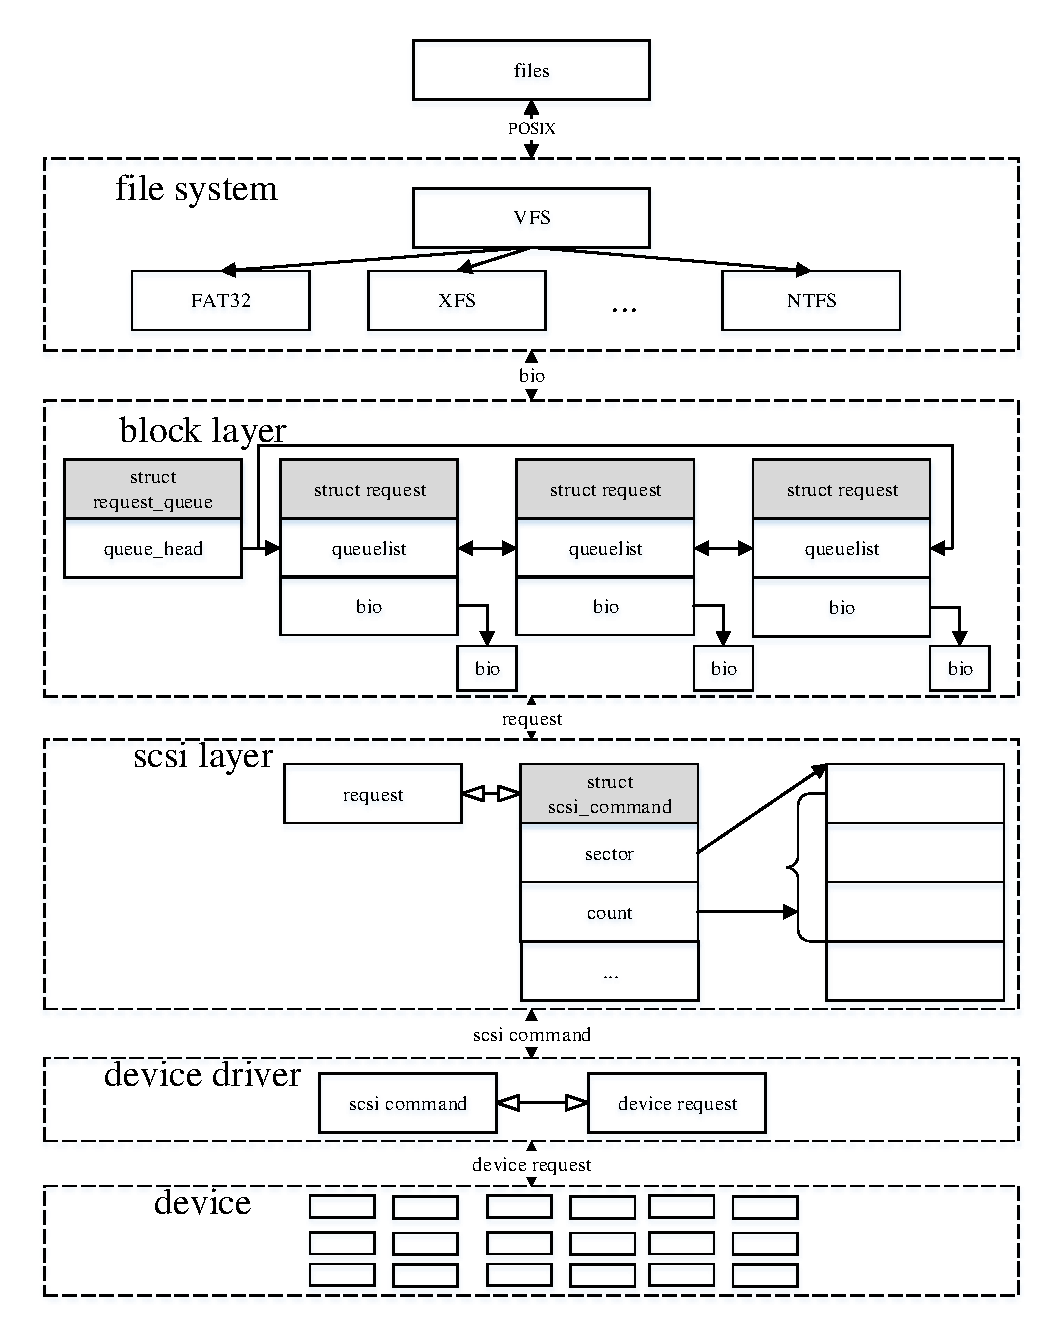
\includegraphics[width=\textwidth]{linux_storage_layer.pdf}
    \bicaption[fig:linux_storage_layer]{Linux存储层次}{Linux存储层次}{Fig}{linux storage layer}
\end{figure}

\subsection{bio}
\label{sec:bio}

bio这一数据结构被用来描述块设备的I/O操作,将内存缓冲区与块设备联系起来的重要桥梁\cite{corbet2005linux}。

bio的具体结构如图\ref{fig:bio}所示。一个bio指针指向由bio结构体组成的链表,bio结构体中的bi\_io\_vec指向一个bi\_vec结构体数组,每个bi\_vec结构体中bv\_page指向内存中的实际页,bv\_offset和bv\_len组合来定位数据在该页中的具体位置,如此,一个bio链表就将散落在内存中的各数据组织为一个块设备请求。

\begin{figure}[!htbp]
    \centering
    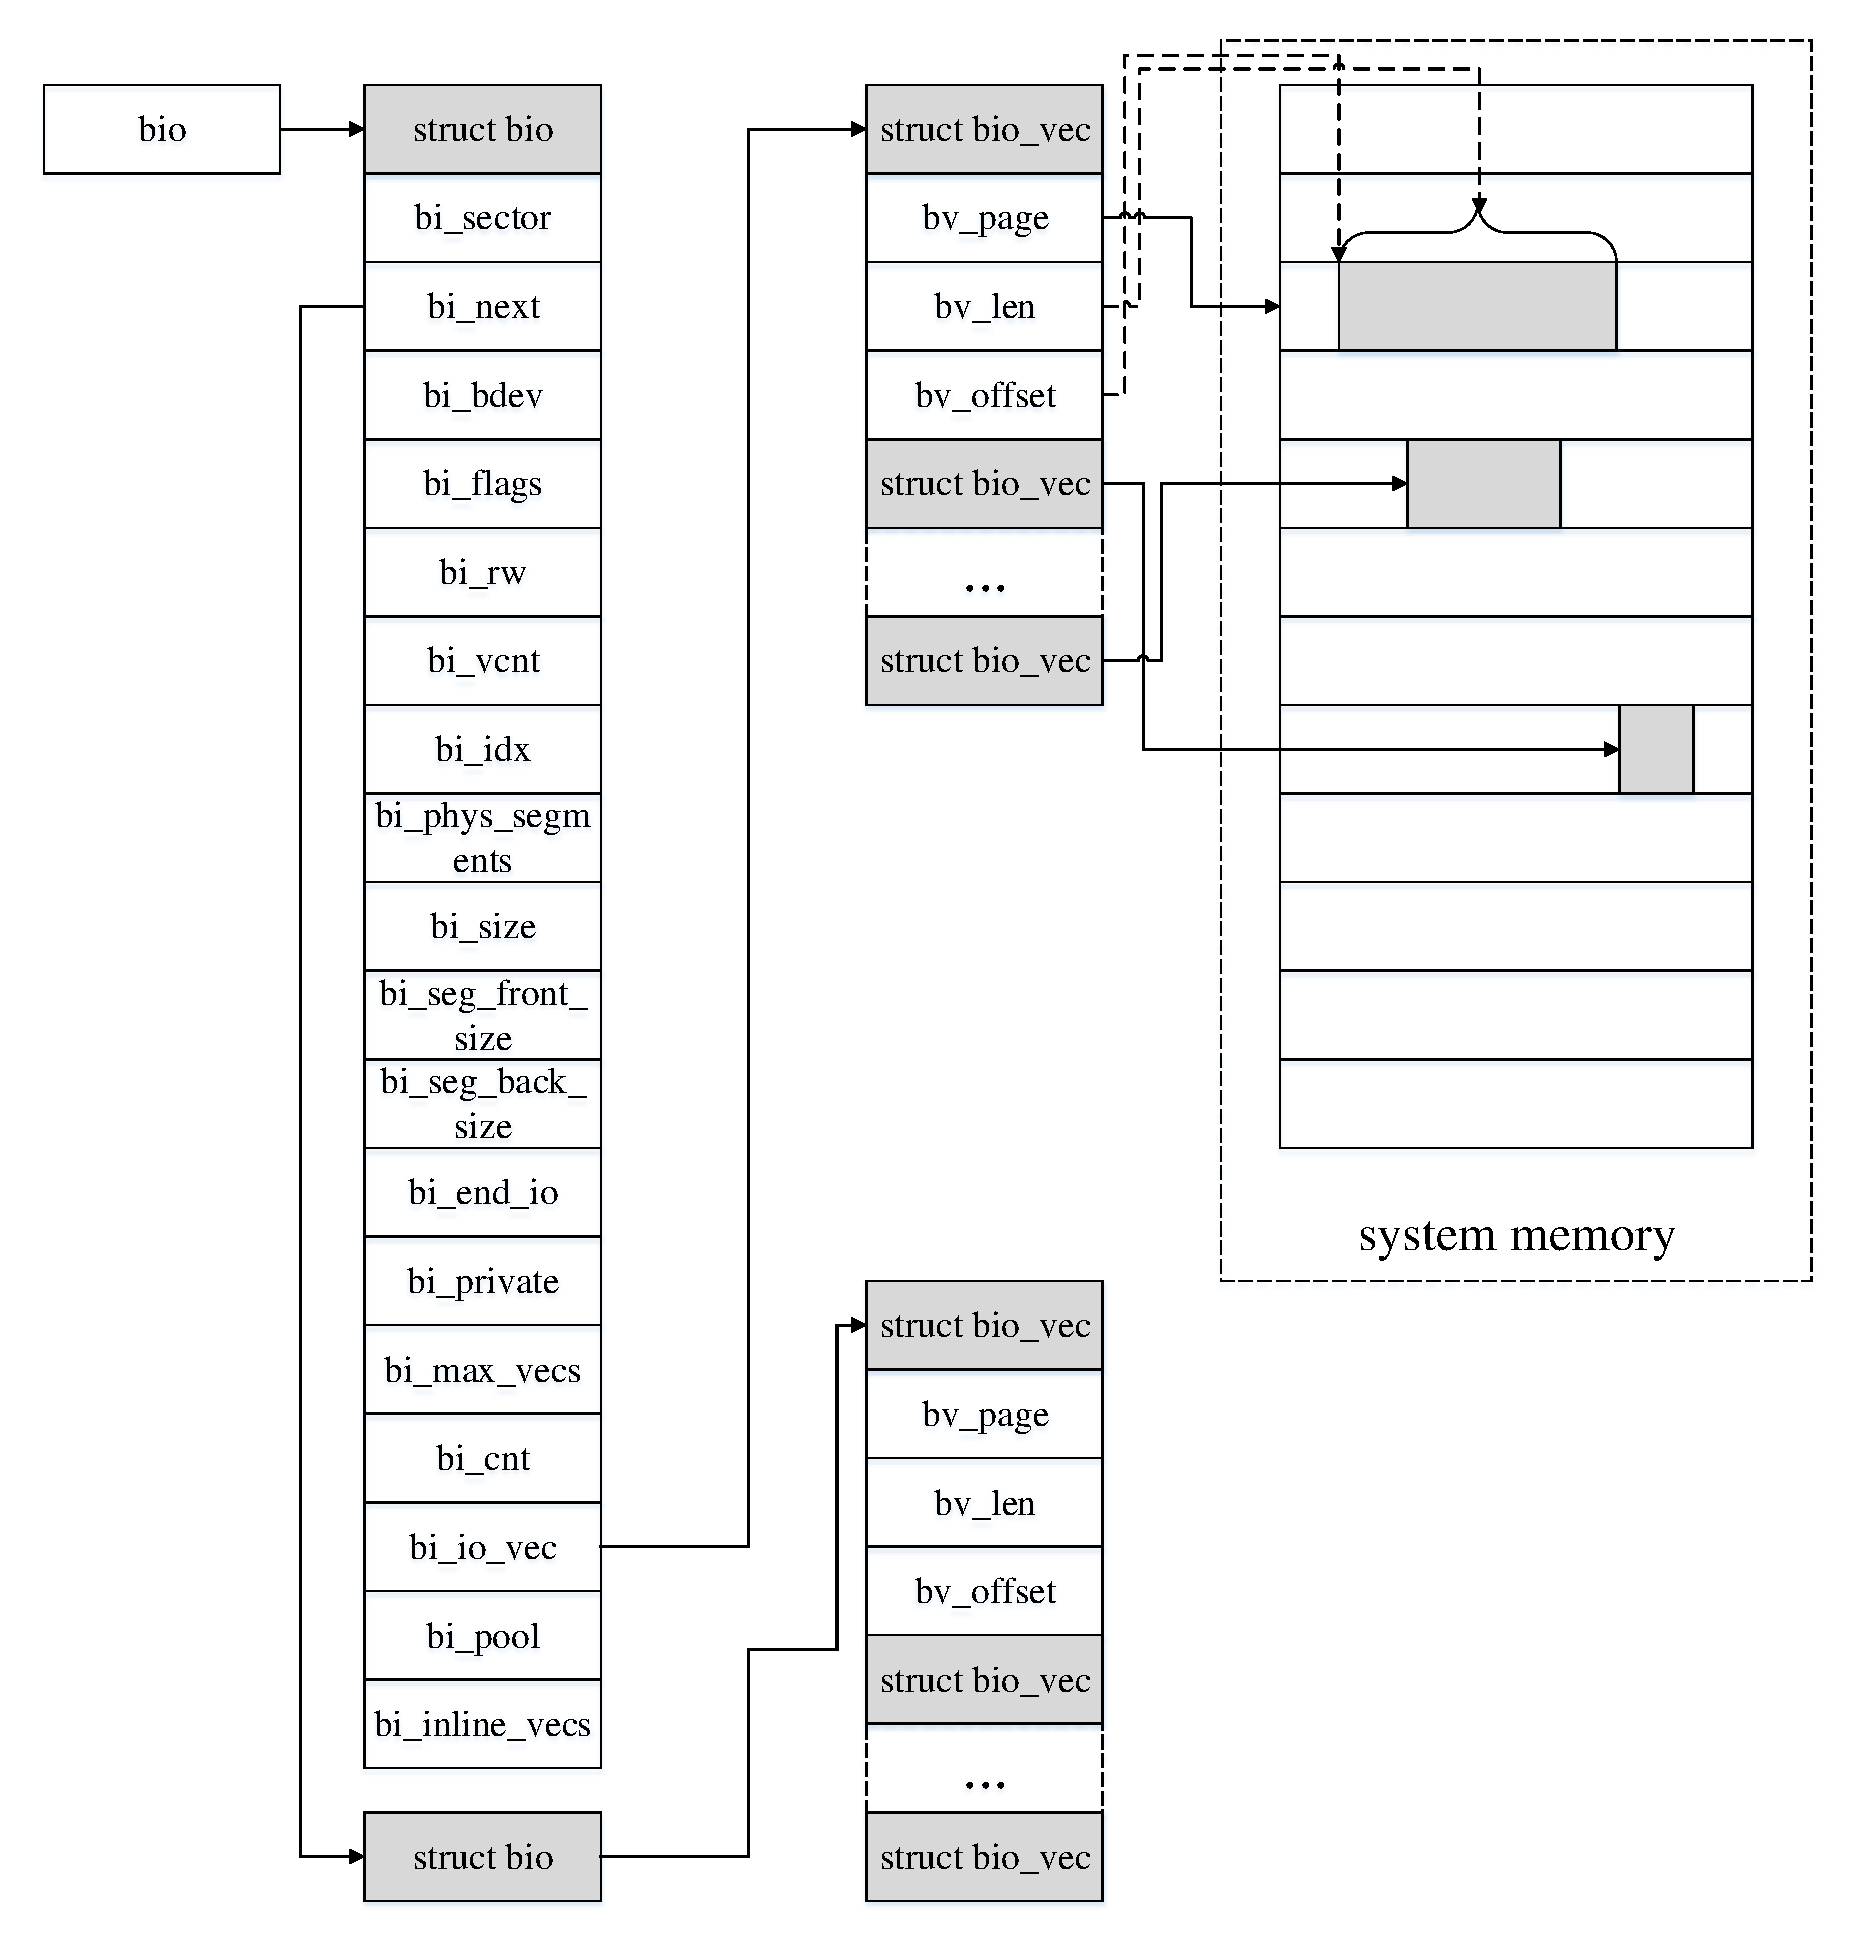
\includegraphics[width=0.8\textwidth]{bio.pdf}
    \bicaption[fig:bio]{bio结构}{bio结构}{Fig}{bio structure}
\end{figure}

\subsection{Device Mapper}

Device Mapper是Linux2.6 内核中支持逻辑卷管理的通用设备映射机制,它为实现用于存储资源管理的块设备驱动提供了一个高度模块化的内核架构\cite{bovet2005understanding}。Device Mapper以一个块设备驱动在内核中注册,它包含mapped device、mapping table、target device这三个重要概念。mapped device可以理解为内核对外提供的逻辑设备,用户看到的也是这个逻辑设备,mapped device通过mapping table组织与与target device的映射关系,一个mapped device可以映射到一个或者多个target device上,总体层次如图\ref{fig:device_mapper}所示,target device可以是真实的物理设备也可以是另一个mapped device,如此迭代,形成一个树状结构。

\begin{figure}[!htbp]
    \centering
    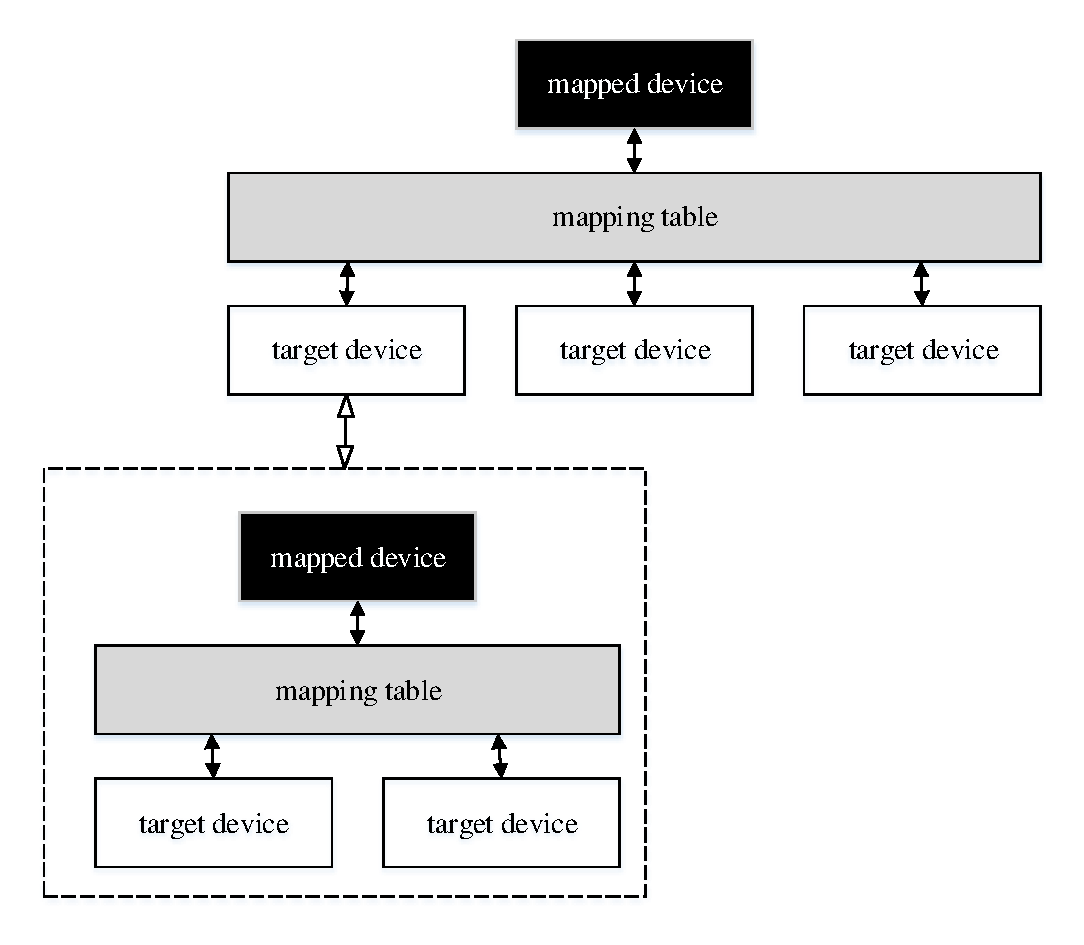
\includegraphics[width=0.8\textwidth]{device_mapper.pdf}
    \bicaption[fig:device_mapper]{Device Mapper层次图}{Device Mapper层次图}{Fig}{Device Mapper Layer}
\end{figure}

Device Mapper的实现原理是将mapped device的make\_request\_fn方法实现为自己的dm\_request,这个经过mapped device的bio请求都会进入dm\_request方法,之后Device Mapper通过判断mapped device是基于request还是基于bio来分别处理:

如果mapped device是基于request的,那么和磁盘设备一样通过generic\_make\_request把bio合并为request,将其放到mapped device的request队列中,当mapped device通过kblockd调用dm\_request\_fn时,dm\_request\_fn中会调用peek\_request从mapped device的request队列中拿出request将其clone(clone生成的request中的bio与原request中的bio指向同一个内存页,clone操作只是分配新的bio和request),然后通过调用map\_request将request映射,将clone后的request发往低层的真实设备。

如果mapped device是基于bio的,那么调用\_dm\_request首先clone bio然后调用\_\_map\_bio将bio映射,将clone后的bio通过generic\_make\_request发往低层的真实设备。

mapped device基于request还是基于bio的主要区别在于,如果是基于request则request是放在mapped device的request队列中,如果是基于bio,则是在调用generic\_make\_request总将bio封装成request放到真实设备的request队列中。


\subsection{其他预备知识}

在qscache系统的实现过程中,除了上面介绍的几个关键知识点外,还涉及很多其他的Linux内核知识,比如Linux的内核模块编程、内核编程中的常用宏、常用数据结构、内核的调试等内容,这里不再详细介绍。

\section{编程实现}

有了上面预备知识的铺垫,就可以比较清楚地介绍qscache系统的编程实现了。下面将着重介绍qscache系统基于Device Mapper机制的系统架构实现、系统信息组织与管理的实现、冷热数据识别算法的实现以及多缓存设备对多后台设备的实现。本系统基于的内核版本为linux 3.10.108。

\subsection{系统架构实现}

qscache系统基于Linux的Device Mapper实现,通过研究Linux内核中Device Mapper的相关代码,本研究发现Device Mapper中使用target\_type这一结构体用来管理对mapped device的各种操作,target\_type的主要成员类型及作用见表\ref{tab:target_type}。因此需要定义qscache对应的target\_type,使qscache系统可以通过Device Mapper组织管理不同设备。

\begin{table}[H]
    \centering
    \bicaption[tab:target_type]{target\_type的主要成员类型及作用}{target\_type的主要成员类型及作用}{Table}{structure of target\_type}
    \begin{tabular}{ccc} 
        \toprule
        成员 & 类型 & 作用\\
        \midrule
        name & const char* & Device Mapper模块的名字 \\ 
        module & struct module* & 对应的Device Mapper模块 \\ 
        version & unsigned[3] & 版本号 \\ 
        ctr & dm\_ctr\_fn & 设备的构造函数 \\ 
        dtr & dm\_dtr\_fn & 设备的析构函数 \\ 
        map & dm\_map\_fn & 指向负责将bio请求重映射的函数 \\ 
        map\_rq & dm\_map\_request\_fn & 指向负责将request请求重映射的函数 \\ 
        end\_io & dm\_endio\_fn & 指向当bio结束时调用的函数 \\ 
        rq\_end\_io & dm\_request\_endio\_fn & 指向当request结束时调用的函数 \\ 
        status & dm\_status\_fn & 指向返回设备状态的函数 \\ 
        message & dm\_message\_fn & 指向负责处理发送给设备的命令的函数 \\ 
        ioctl & dm\_ioctl\_fn & 指向负责处理通过ioctl对设备管理的函数 \\ 
        iterate\_devices & dm\_iterate\_devices\_fn & 指向负责遍历处理与设备相关的设备的函数 \\ 
        \bottomrule
    \end{tabular}
\end{table}

另外qscache系统对于I/O带宽按权限进行分配的功能将通过使用Linux自带的I/O调度器的CFQ策略,通过为不同进程设置不同的cgroup的weight实现对这些进程按照权重不同分配不同的I/O带宽,但是由于I/O调度器只对request队列起作用,对bio不起作用,因此qscache系统将实现基于bio模式启动与基于request模式启动,对于不同的模式分别定义不同的target\_type然后在模块加载时注册不同的target\_type就以不同模式启动了。但是本研究发现现有的Device Mapper提供的target\_type并不能很好地实现基于request的模式,因此下面将分别对基于bio模式与基于request模式的公用接口函数的实现、基于bio模式的实现以及基于request模式的实现展开详细介绍。

\subsubsection{公用接口函数的实现}

qscache系统的公用接口函数为ctr、dtr、status、ioctl、iterate\_devices这五个,下面将分别进行介绍。

ctr接口的实现流程如图\ref{fig:qscache_ctr}所示,ctr负责接收用户传来的各种参数,对相关结构体进行内存的申请工作,对相关的工作队列、等待队列等进行初始化操作,以及对相关参数进行设置,当操作出错时释放已申请的内存空间并返回。

\begin{figure}[H]
    \centering
    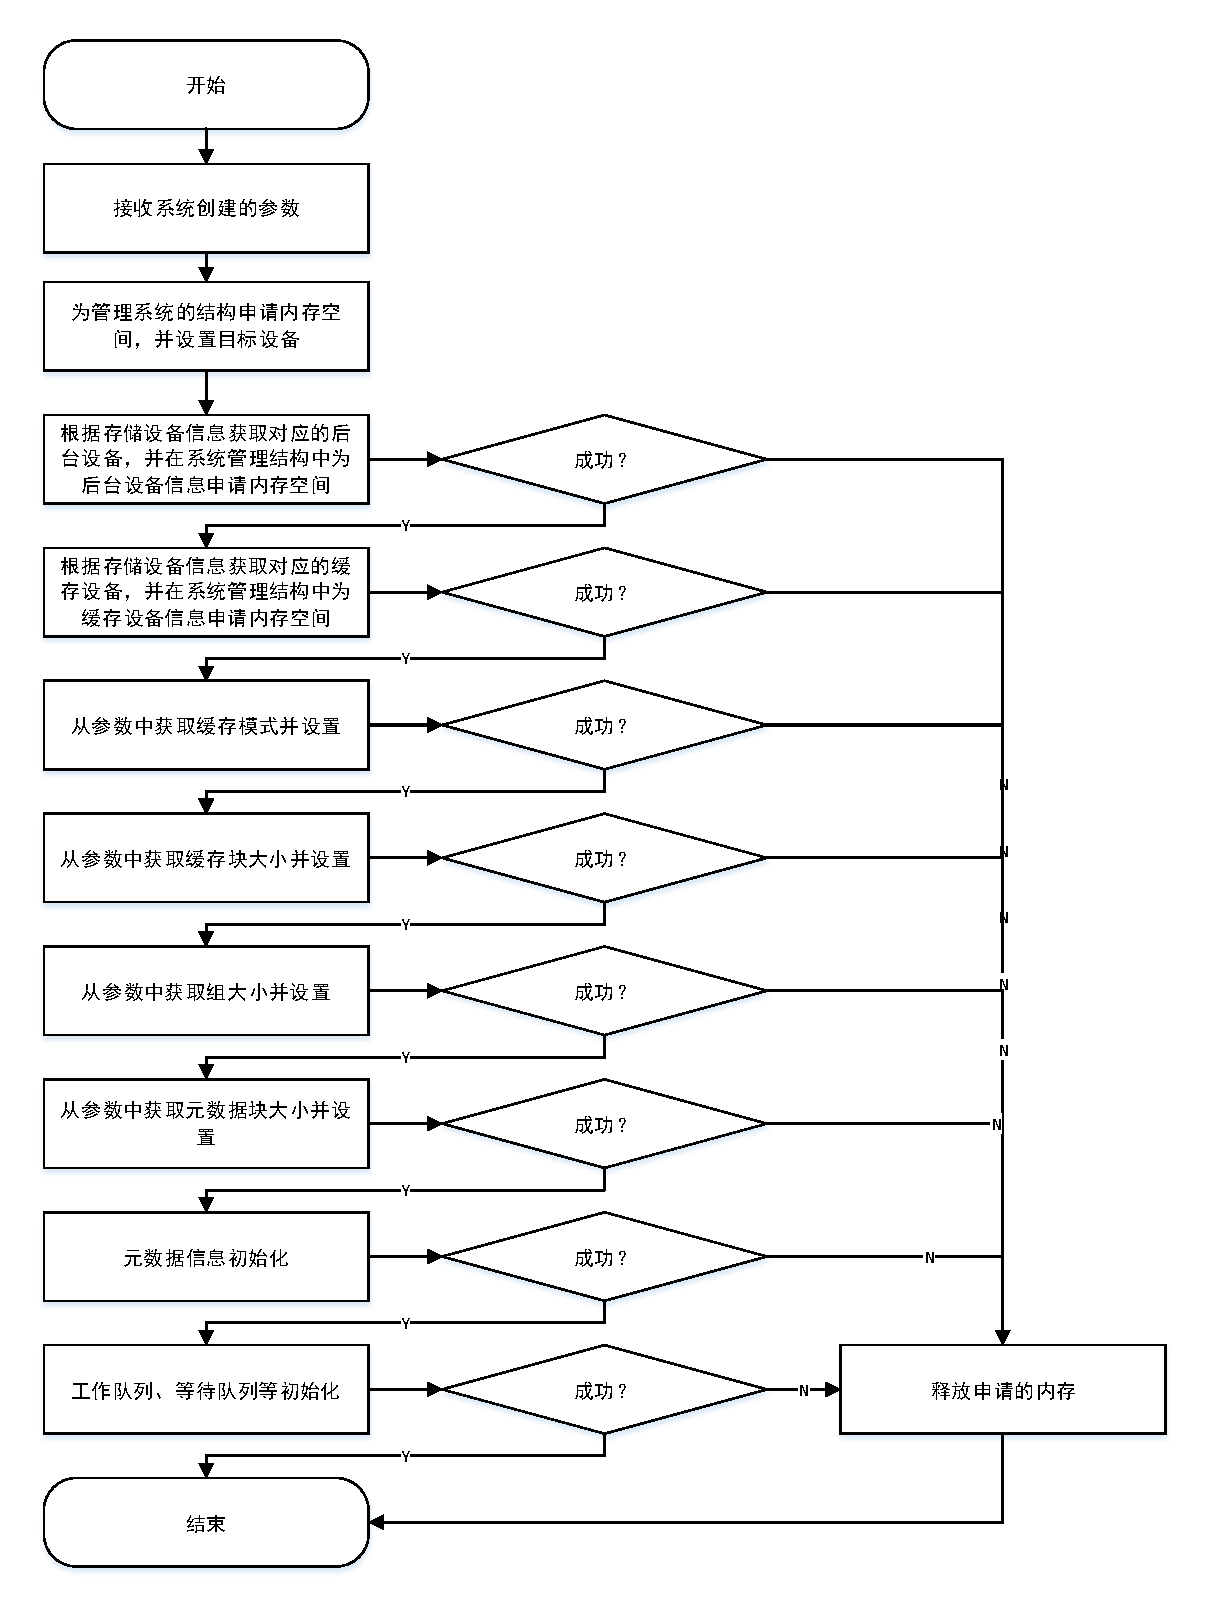
\includegraphics[width=0.8\textwidth]{qscache_ctr.pdf}
    \bicaption[fig:qscache_ctr]{qscache的ctr接口}{qscache的ctr接口}{Fig}{process of qscache ctr}
\end{figure}

dtr接口的实现比较简单,就是将在ctr接口中申请的各种资源依倒序依次释放,保证系统占用的资源都返还操作系统,不会发生内存泄露的情况。

status接口负责根据系统记录的信息返回系统的当前状态供用户查询,通过status接口,用户可以得到读命中次数、写命中次数、脏数据命中次数、缓存块替换次数、对缓存设备的读写次数、对后台设备的读写次数、缓存设备的容量使用情况、后台设备的容量使用情况、未缓存的操作数等信息。

ioctl接口负责处理通过ioctl对设备的管理操作,主要接收用户传来的参数对系统的进程黑名单和进程白名单进行增删操作。

iterate\_devices接口负责遍历系统所管理的缓存设备和后台设备,对它们调用指定的函数。

\subsubsection{基于bio模式的实现}

基于bio模式的实现主要是target\_type中map接口的实现,map是整个系统数据的入口,map负责对bio请求进行解析,并根据请求的操作类型分别交由不同函数处理。

对于读请求的处理如图\ref{fig:qscache_map_read}所示。首先判断请求是否为可以被缓存的请求,判断的依据是判断进程是否在黑名单中以及依据参数的设置决定是否要缓存顺序请求,如果不能被缓存则直接提交到后台设备执行读操作,如果可以被缓存,则首先在缓存设备中查找数据块,如果找到对应数据块,则将请求提交到缓存上执行读操作,如果没有找到数据块,则将请求提交到后台设备上执行读操作,并根据操作是否可以被缓存以及数据块的热度决定是否要替换缓存块执行对应的缓存块操作。

\begin{figure}[H]
    \centering
    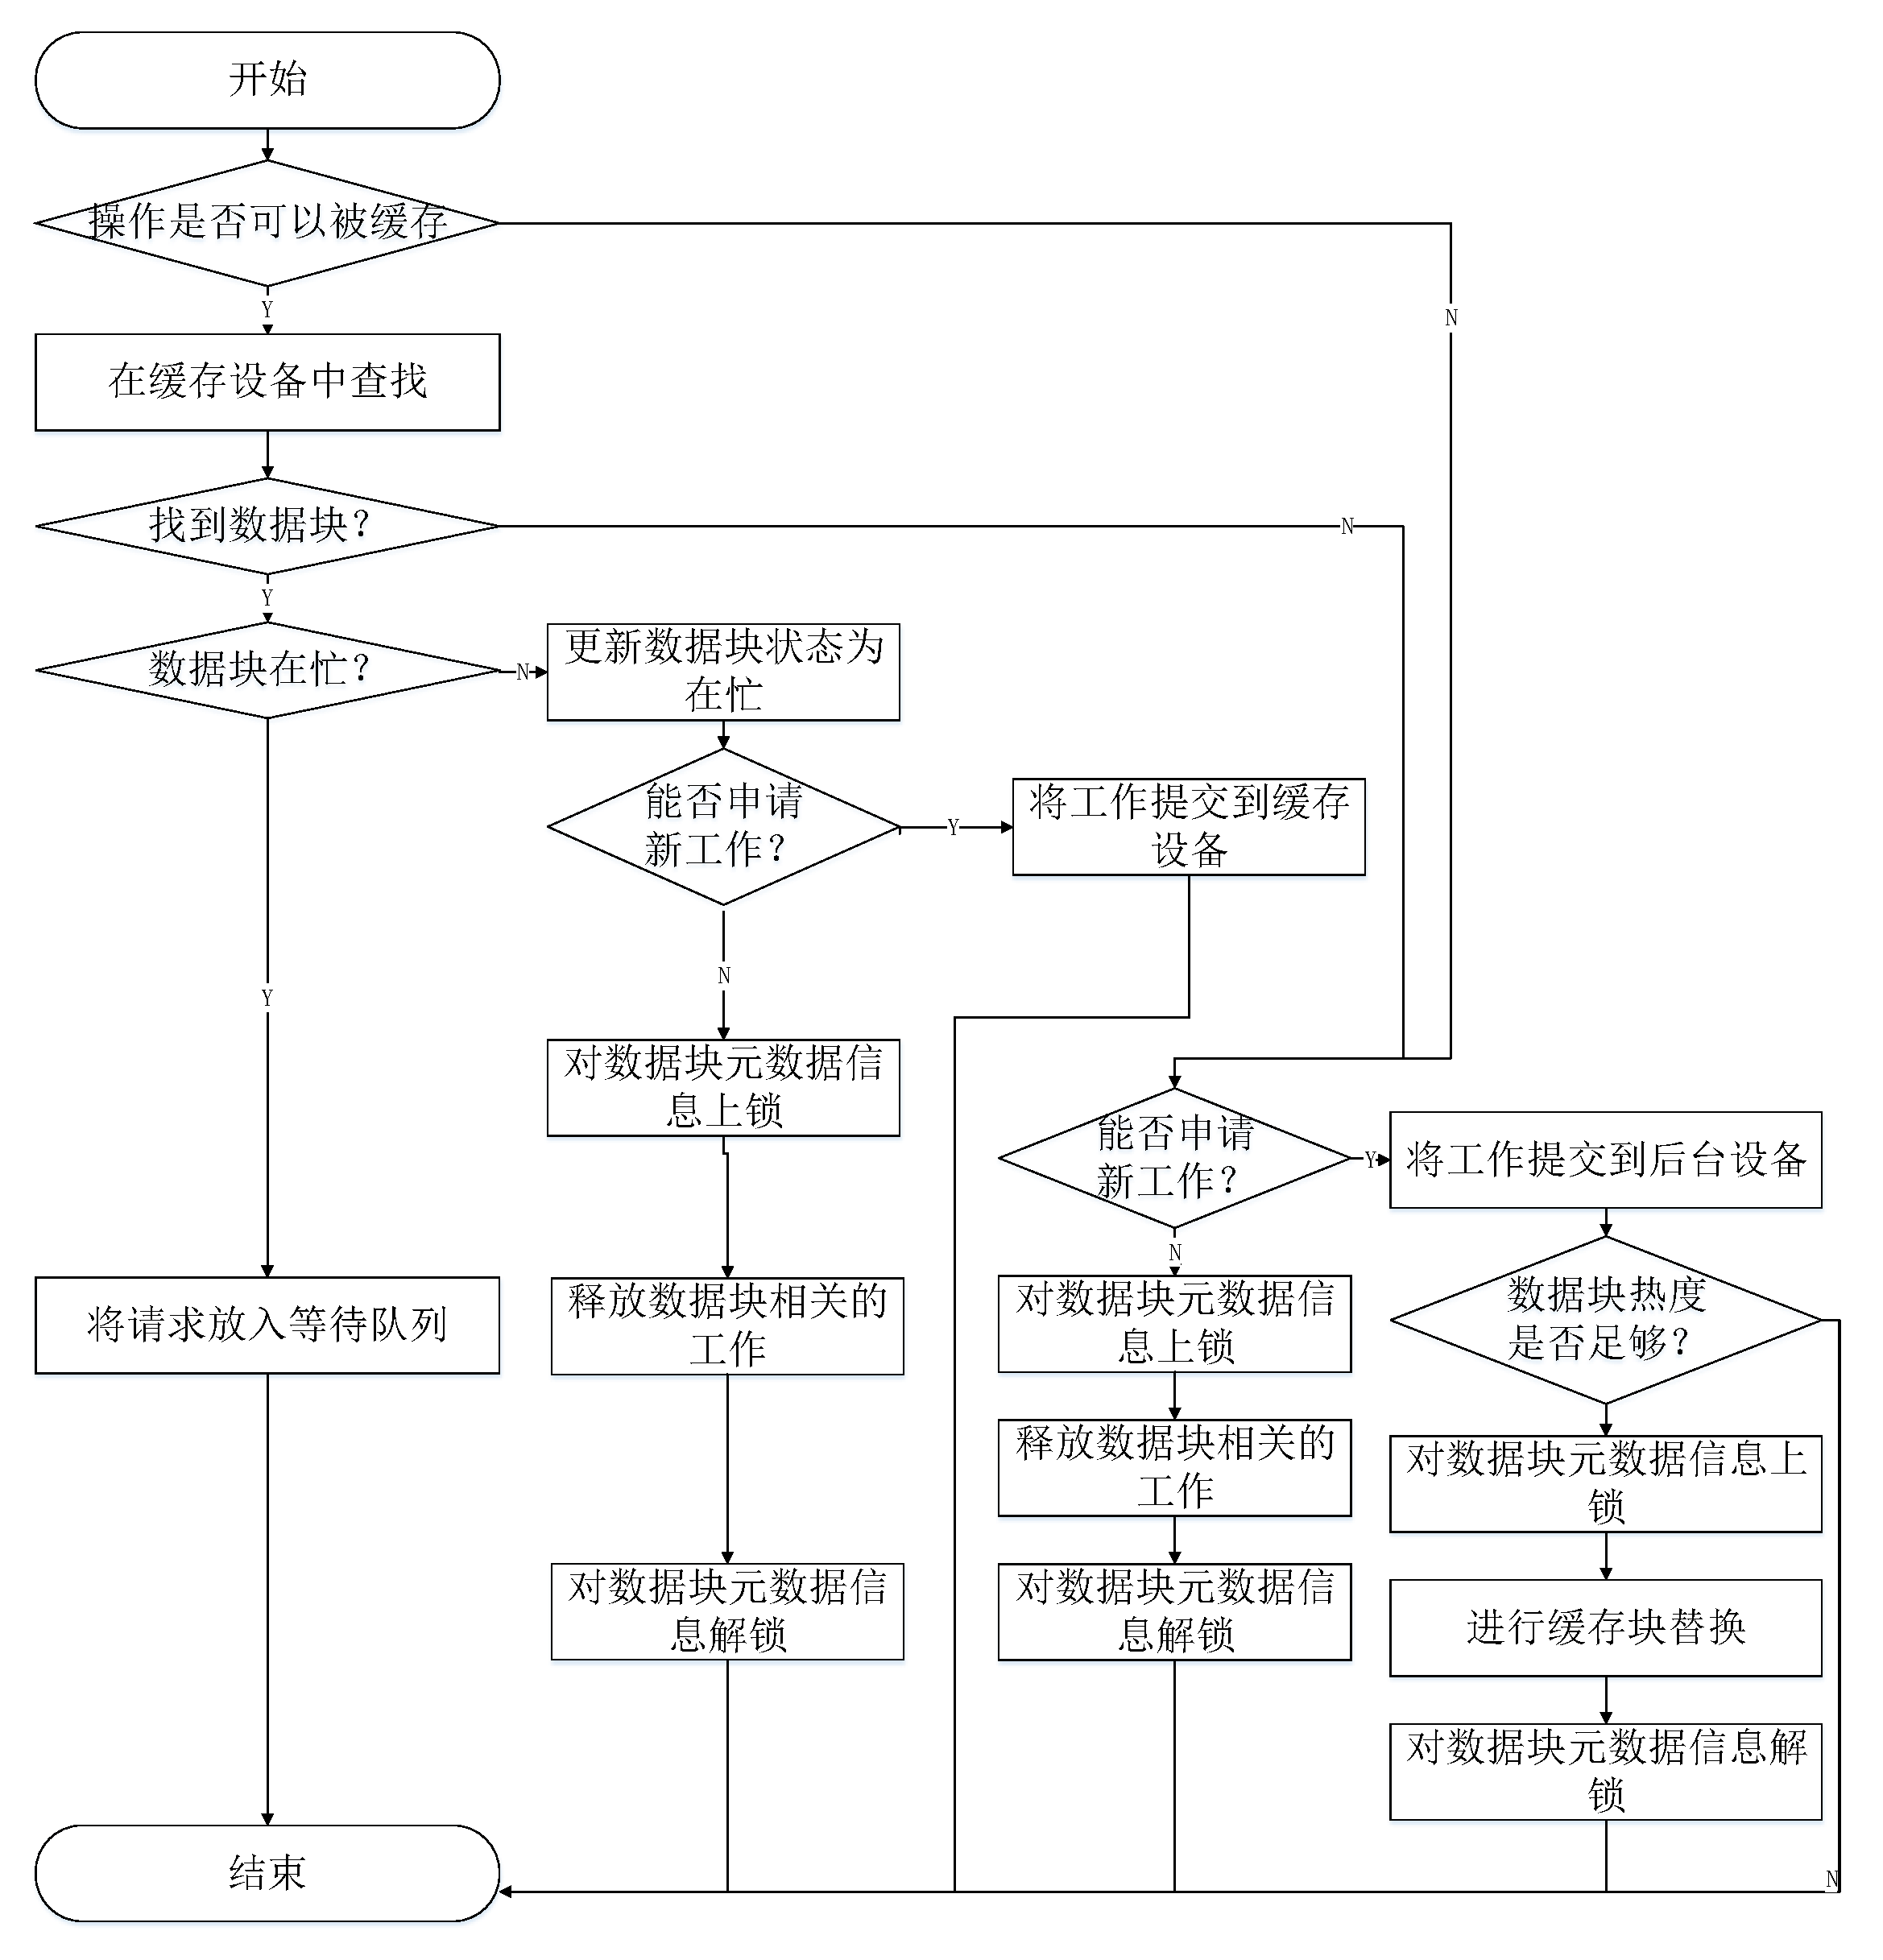
\includegraphics[width=0.8\textwidth]{qscache_map_read.pdf}
    \bicaption[fig:qscache_map_read]{qscache的map接口读请求处理}{qscache的map接口读请求处理}{Fig}{process of qscache map read}
\end{figure}

对于写请求的处理如图\ref{fig:qscache_map_write}所示。首先判断请求是否为可以被缓存的请求,判断的依据是判断进程是否在黑名单中以及依据参数的设置决定是否要缓存顺序请求,如果不能被缓存则直接提交到后台设备执行写操作,如果可以被缓存,则首先在缓存设备中查找数据块,如果找到对应数据块,则将请求提交到缓存上执行写操作,并判断是否为写穿模式,如果为写穿模式则也将请求提交到后台设备上执行写操作,如果没有找到数据块,则将请求提交到后台设备上执行写操作,并根据操作是否可以被缓存以及数据块的热度决定是否要替换缓存块执行对应的缓存块操作。

\begin{figure}[H]
    \centering
    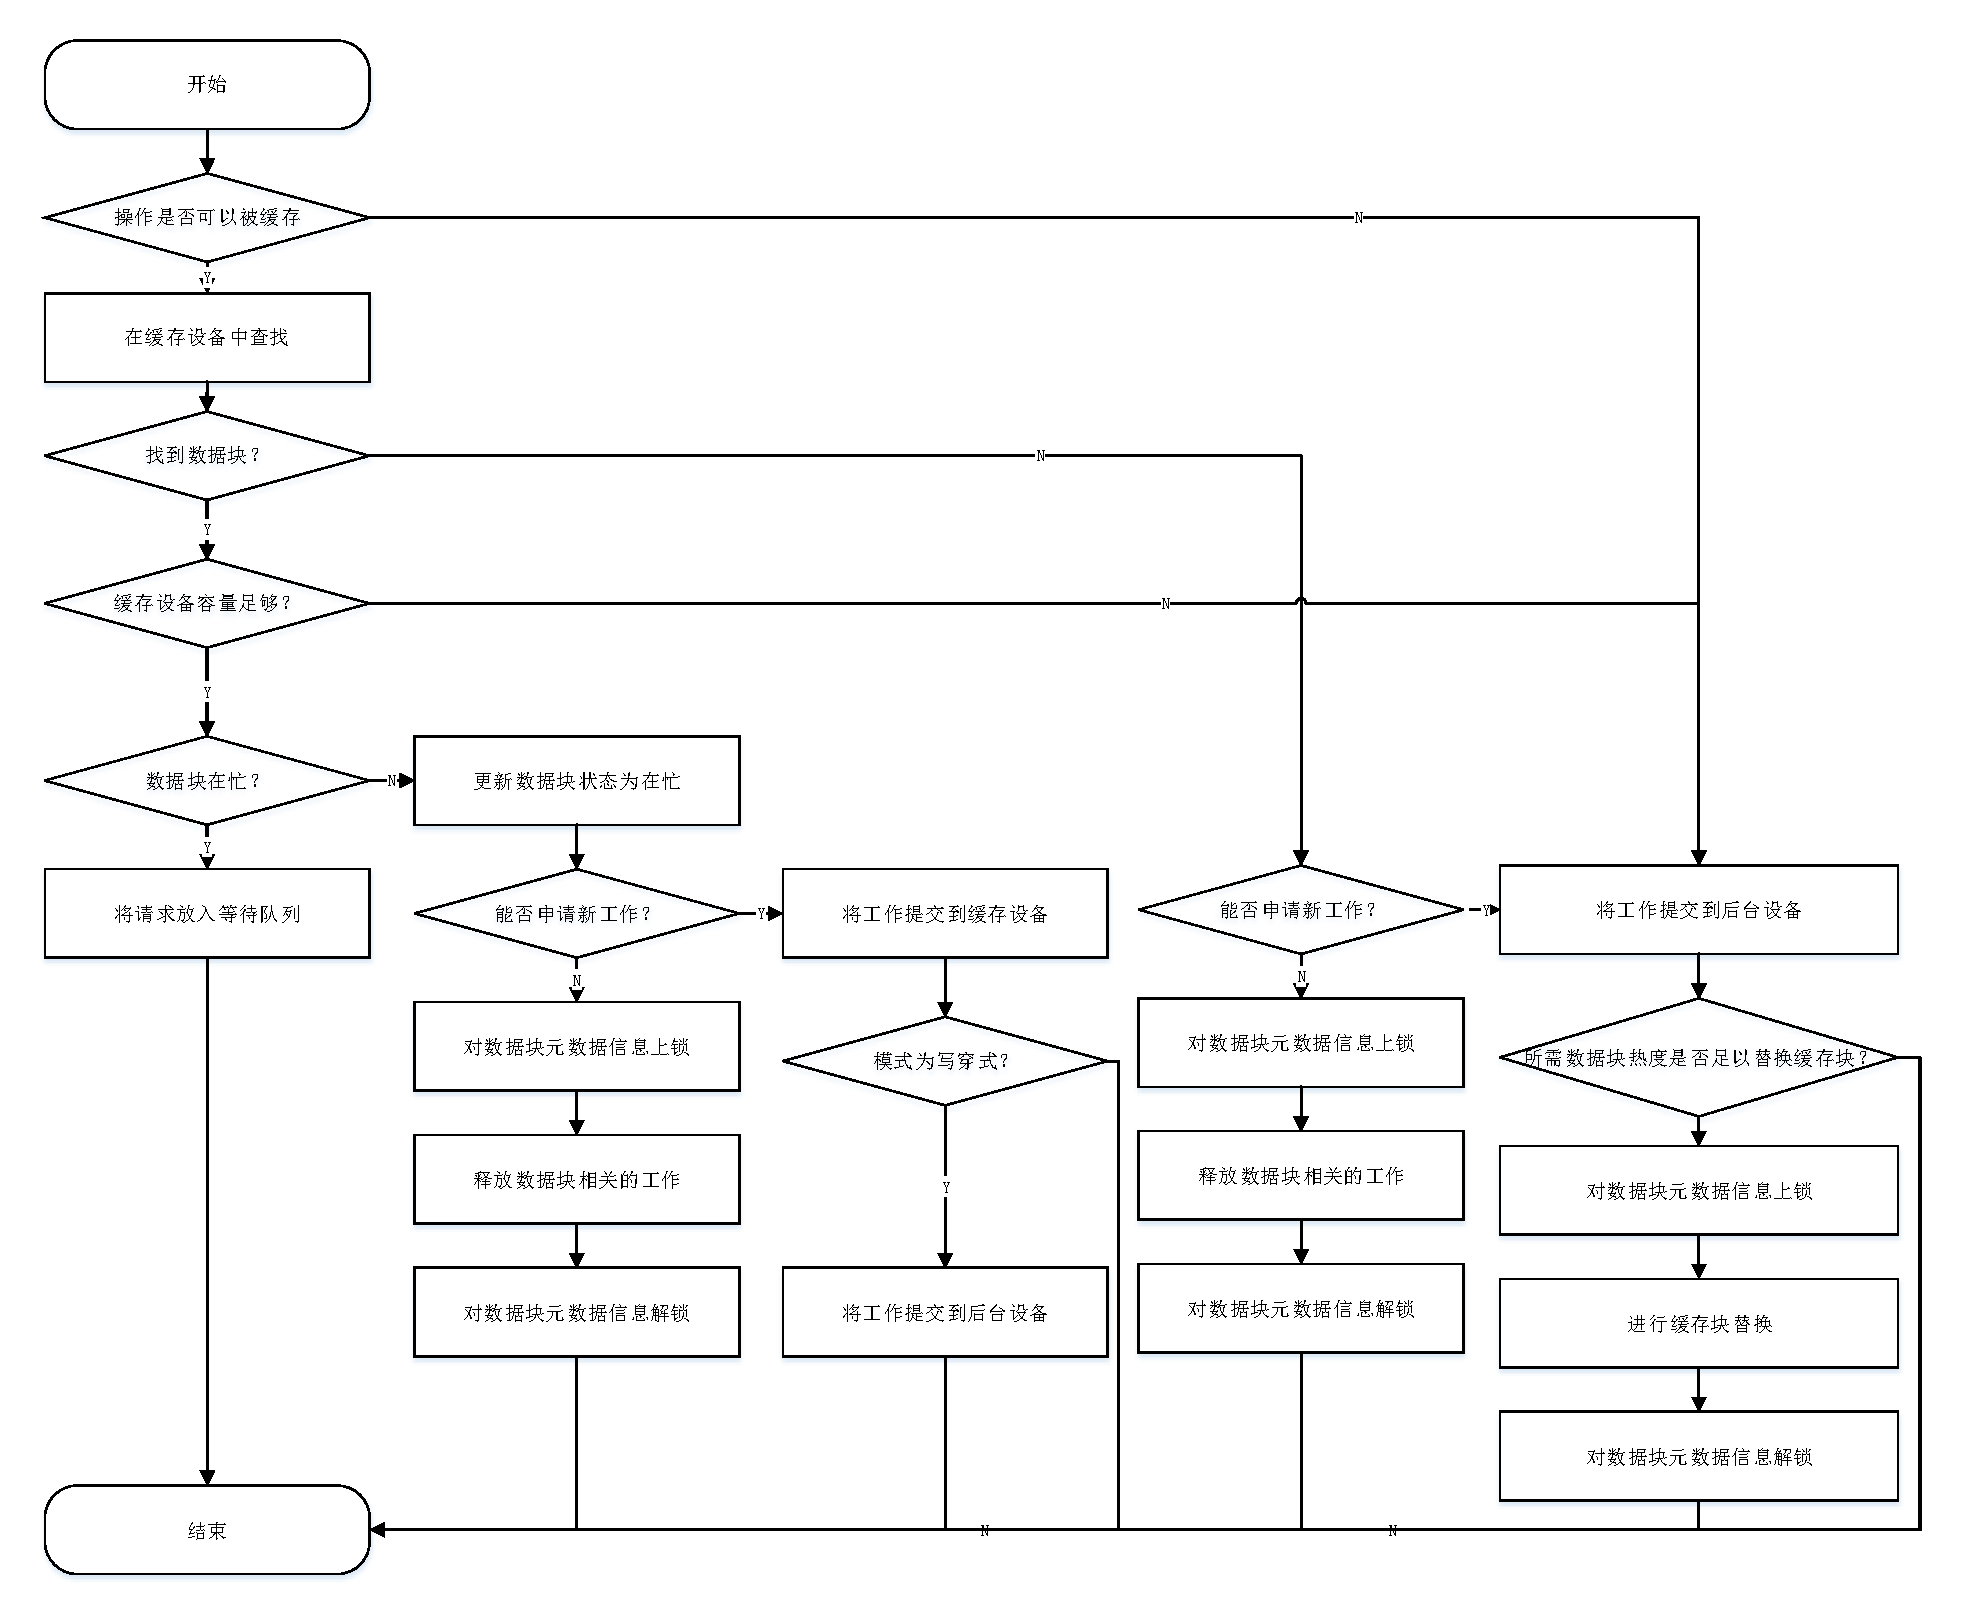
\includegraphics[width=0.8\textwidth]{qscache_map_write.pdf}
    \bicaption[fig:qscache_map_write]{qscache的map接口写请求处理}{qscache的map接口写请求处理}{Fig}{process of qscache map write}
\end{figure}

\subsubsection{基于request模式的实现}

本研究发现现有的Device Mapper的实现中,仅有multipath\_target是基于request的target\_type,而在multipath\_target中map\_rq的实现multipath\_map仅仅是改变request队列然后返回DM\_MAPIO\_REMAPPED,而混合存储系统中map\_rq必须负责将对mapped device的请求映射到低层的设备因此不能仅仅像multipath\_target中map\_rq的实现一样简单。因此需要实现一个新的接口。在target\_type中添加mk\_rq接口实现用bio生成request,然后依靠map\_rq将请求映射到不同的低层设备。

对Linux的内核作出的具体修改如下:

\begin{enumerate}
    \item include/linux/dm-io.h文件对dm\_io\_request结构体添加三个变量,submit\_bio用以表示是否直接提交bio,start和end为两个bio指针,指向该dm\_io\_request的起始bio和终止bio。
    \item drivers/md/dm-io.c文件,do\_region改为接收dm\_io\_request类型参数,依据dm\_io\_request类型的参数中submit\_bio的设置判断是直接提交bio还是放入request中。dispatch\_io改为接收dm\_io\_request类型参数,相关操作包括对do\_region的调用相应改为基于dm\_io\_request类型的操作。sync\_io改为接收dm\_io\_request类型参数,相关操作包括对dispatch\_io的调用相应改为基于dm\_io\_request类型的操作。async\_io改为接收dm\_io\_request类型参数,相关操作包括对dispatch\_io的调用相应改为基于dm\_io\_request类型的操作。dm\_io中对sync\_io和async\_io的调用都改为传递dm\_io\_request类型参数。
    \item include/linux/device-mapper.h文件中对target\_type结构体添加函数指针mk\_rq作为新的新接口,用以支持自己对request的生成。
    \item drivers/md/dm.c文件,dm\_request原本只是简单地判断mapped device是基于request还是基于bio,并据此分别调用blk\_queue\_bio或\_dm\_request。现在首先从映射表中获得mapped device,查看是否实现了具体的mk\_rq方法,如果实现了则调用该方法然后返回,否则依旧根据是基于request还是基于bio分别调用blk\_queue\_bio或\_dm\_request,流程如图\ref{fig:dm_request}所示。

    \begin{figure}[!htbp]
        \centering
        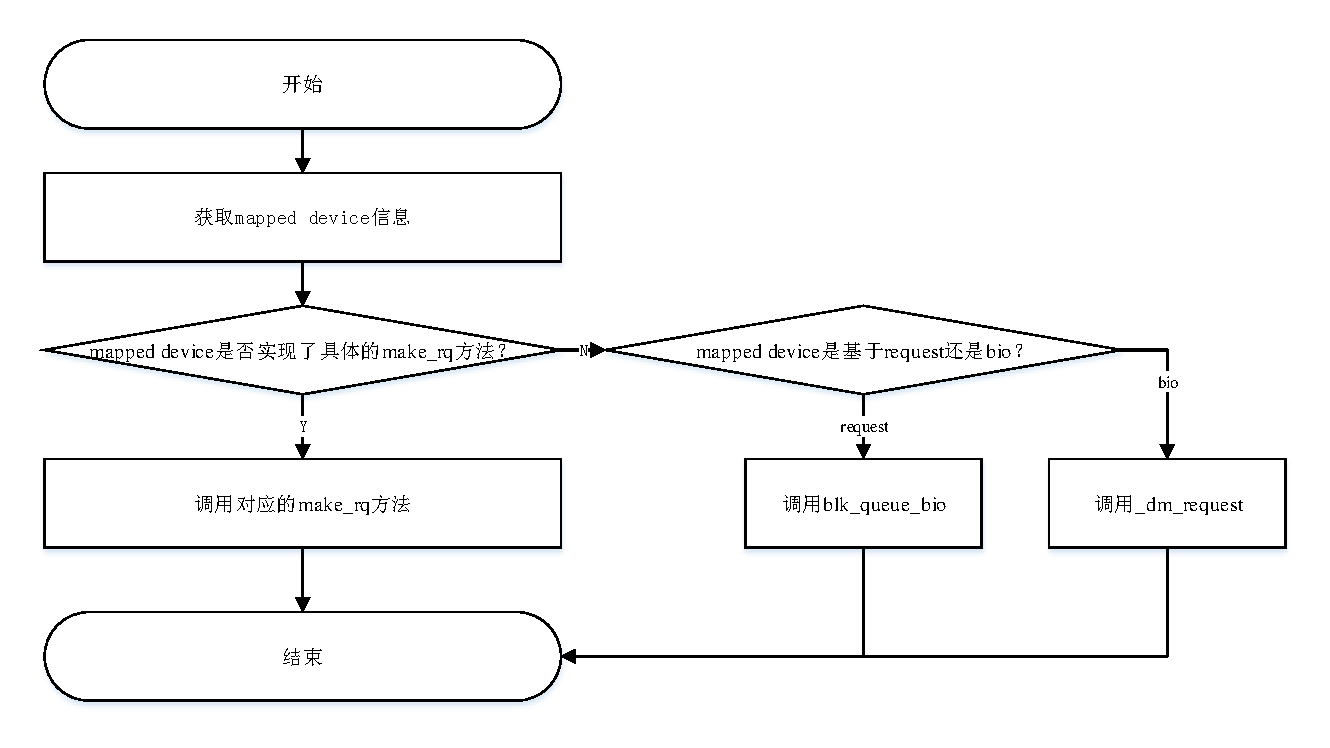
\includegraphics[width=\textwidth]{dm_request.pdf}
        \bicaption[fig:dm_request]{dm\_request处理流程}{dm\_request处理流程}{Fig}{dm\_request process}
    \end{figure}

    \item drivers/md/dm-bufio.c文件,use\_dmio和dm\_bufio\_issue\_flush中初始化io\_req时设置submit\_bio为1,默认直接提交bio。
    \item drivers/md/dm-kcopyd.c文件,run\_io\_job中初始化io\_req时设置submit\_bio为1,默认直接提交bio。
    \item drivers/md/dm-log.c文件,create\_log\_context中设置lc的io\_req的submit\_bio为1,默认直接提交bio。
    \item drivers/md/dm-raid1.c文件,mirror\_flush、read\_async\_bio和do\_write中初始化io\_req时设置submit\_bio为1,默认直接提交bio。
    \item drivers/md/dm-snap-persistent.c文件,chunk\_io中初始化io\_req时设置submit\_bio为1,默认直接提交bio。
\end{enumerate}

在对Linux内核修改完毕后,现在的Device Mapper中target\_type支持开发者实现自己的mk\_rq接口。qscache系统通过实现mk\_rq和map\_rq接口实现基于request的混合存储系统,具体流程如图\ref{fig:request_process}所示。mk\_rq()负责用bio生成对应的request而map\_rq()负责将对混合存储系统的请求分派到具体的实际设备执行操作。

\begin{figure}[!htbp]
    \centering
    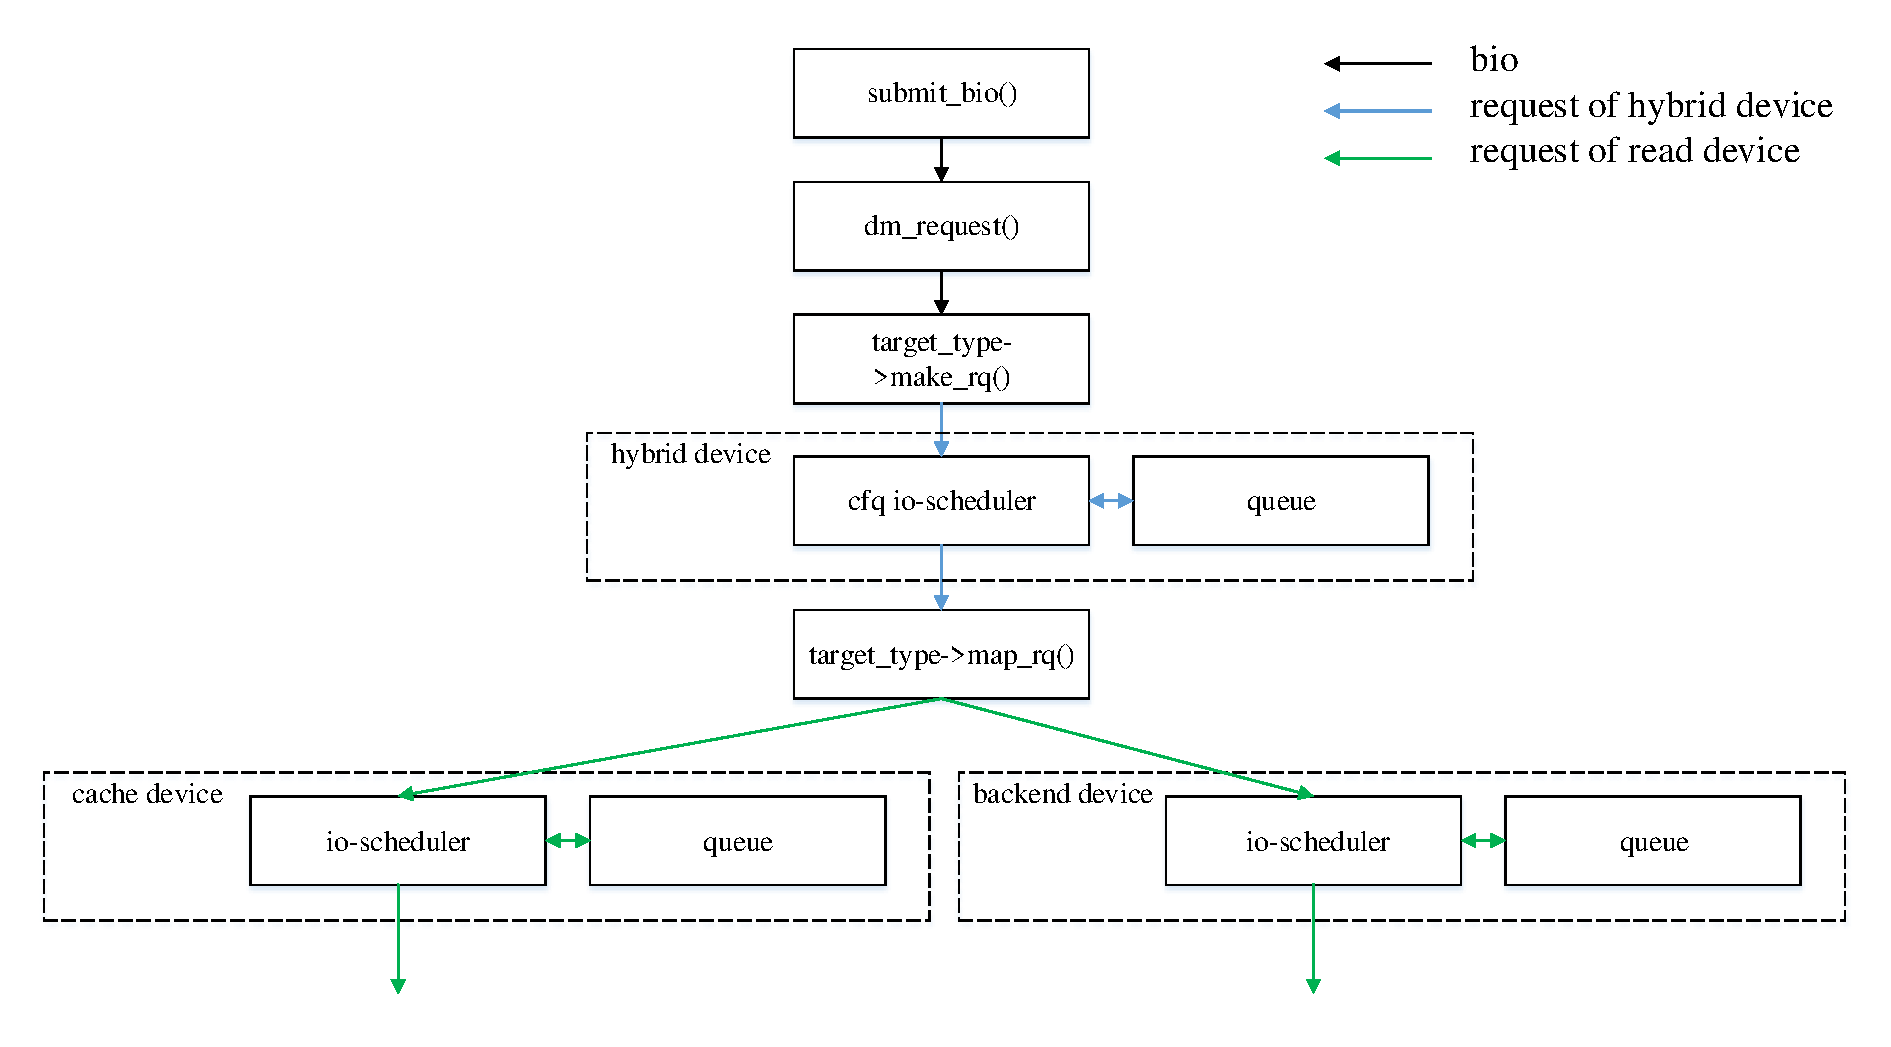
\includegraphics[width=0.9\textwidth]{request_process.pdf}

    \vskip -1cm

    \bicaption[fig:request_process]{基于request的请求流程}{基于request的请求流程}{Fig}{request process in request-based system}
\end{figure}

具体地说,mk\_rq()接收对系统的bio请求,然后根据bio判断对系统的具体操作,然后去调用对应操作的函数并传入参数设置不立即提交bio,各操作函数经过递归调用最后都会落到dm\_io\_async\_bvec()中,如图\ref{fig:dm_io_async_bvec}所示,mk\_rq()不论是调用不经缓存的操作,还是缓存命中或未命中的读写操作最终都会调用dm\_io\_async\_bvec(),并在mk\_rq()中将是否立即提交bio的参数一路传给dm\_io\_async\_bvec()。dm\_io\_async\_bvec()根据传入的参数生成dm\_io\_request并调用dm\_io(),对于立即提交的bio,dm\_io\_async\_bvec()结束调用后就立刻返回,对于不是立即提交的bio,再dm\_io()中会设置整个bio的开始与结束,然后返回dm\_io\_async\_bvec()通过开始与结束遍历这些bio,然后用这些bio各自或生成一个request放入队列中。

\begin{figure}[!htbp]
    \centering
    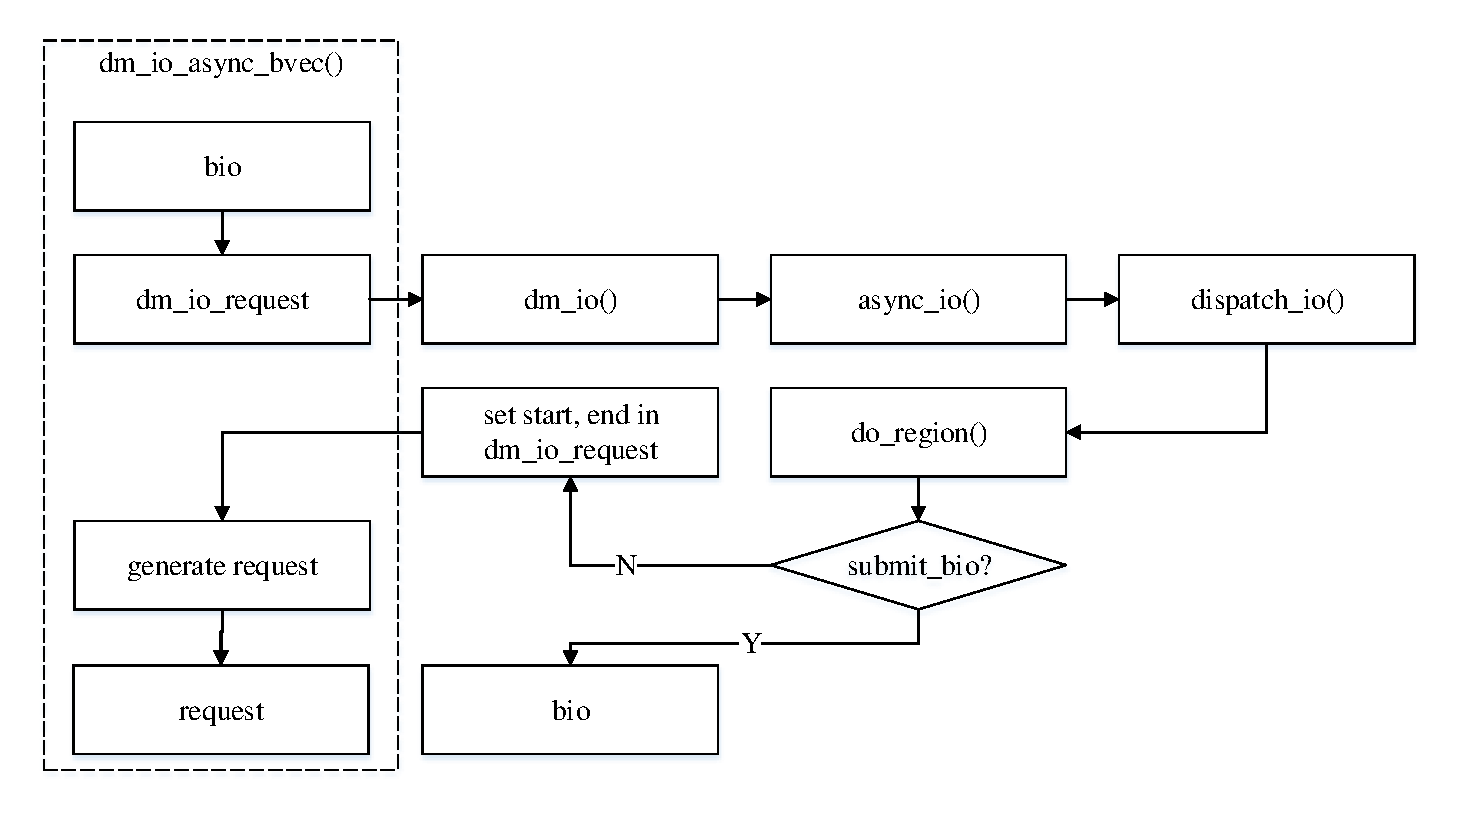
\includegraphics[width=\textwidth]{dm_io_async_bvec.pdf}
    \bicaption[fig:dm_io_async_bvec]{dm\_io\_async\_bvec()调用以及处理流程}{dm\_io\_async\_bvec()调用以及处理流程}{Fig}{call and process of dm\_io\_async\_bvec()}
\end{figure}


\subsection{系统信息组织与管理的实现}

qscache系统的系统信息由一个全局的数据结构cache\_c进行统一管理。cache\_c中的主要成员类型及其作用如表\ref{tab:cache_c}所示。其他诸如黑名单、白名单也在cache\_c中。相关冷热数据识别要用到的数据结构,则以set为单位存放在cache\_sets这一结构体中。

\begin{table}[!htbp]
    \centering
    \bicaption[tab:cache_c]{cache\_c的主要成员类型及作用}{cache\_c的主要成员类型及作用}{Table}{structure of cache\_c}
    \begin{tabular}{ccc} 
        \toprule
        成员 & 类型 & 作用\\
        \midrule
        tgt & struct dm\_target* & Device Mapper中对target\_type的一层封装 \\ 
        disk\_dev & struct dm\_dev* & 管理与后台设备相关的信息 \\ 
        cache\_dev & struct dm\_dev* & 管理与缓存设备相关的信息 \\ 
        cache & struct cacheblock* & 管理缓存块的哈希表 \\ 
        cache\_sets & struct cache\_set* & 用于管理set \\ 
        size & sector\_t & 缓存大小 \\ 
        assoc & unsigned int & 缓存设备的set大小 \\ 
        block\_size & unsigned int & 缓存块的大小 \\ 
        disk\_assoc & unsigned int & 后台设备的set大小 \\ 
        num\_sets & unsigned int & set的数目 \\ 
        cache\_mode & int & 缓存模式:写回、写穿等 \\ 
        dirty\_thresh\_set & int & 每个set开始写回脏数据的阈值 \\ 
        max\_clean\_ios\_set & int & 每个set写回脏数据的量的阈值 \\ 
        dm\_vdevname & char[DEV\_PATHLEN] & 虚拟出来的设备名 \\ 
        cache\_devname & char[DEV\_PATHLEN] & 缓存设备的UUID \\ 
        disk\_devname & char[DEV\_PATHLEN] & 后台设备的UUID \\ 
        bypass\_cache & int & 是否略过缓存 \\      
        \bottomrule
    \end{tabular}
\end{table}

\subsection{冷热数据识别算法的实现}

在qscache系统中采用双层LRU链表,具体思想见\ref{sec:data_hot_identification}。系统为每个set建立两个LRU链表,在管理cache的cache\_sets结构体中使用四个变量hotlist\_lru\_head,hotlist\_lru\_tail,warmlist\_lru\_head,warmlist\_lru\_tail描述这两个链表。对于链表中数据的移动只需要更改对应的指针即可。对于后台设备的数据块访问,将该数据块放到warmlist的尾端,当对该数据块的访问达到一定阈值时,将其移到hotlist的尾端,当要发生缓存块替换时,从warmlist的尾端移出数据块,并把hotlist的尾端放入warmlist中。

\subsection{多缓存设备对多后台设备的实现}

在\ref{sec:multi-cache_to_multi-backend}中提到qscache系统采用分层管理结构,将多设备的管理与混合存储系统隔离开。qscache系统对多缓存设备对多后台设备的实现基于LVM。将以多缓存设备与多后台设备创建混合存储系统封装成用户态的工具,使之对用户透明,首先接收用户提供的缓存设备信息、后台设备信息、系统参数,然后依据参数先将多个SSD映射为一个虚拟缓存设备,再将多个HDD映射为一个虚拟后台设备,最后将这两个设备的信息连同混合存储系统的配置参数发给dmsetup命令,dmsetup将参数传给系统在内核的初始化函数进行混合存储系统的构建。系统的销毁同样封装为对用户透明的用户态工具,首先调用系统在内核的注销函数销毁混合存储系统,然后清理在虚拟缓存设备上残留的数据,之后将虚拟缓存设备卸载解除与多个SSD的映射关系,再将虚拟后台设备卸载解除与多个HDD的映射关系。


\section{本章小结}
本章介绍了qscache系统在实现中需要的预备知识以及具体的实现方法。预备知识主要介绍了Linux存储层次、bio和Device Mapper。具体的实现方法主要介绍了基于Device Mapper机制的系统架构实现、系统信息组织与管理的实现、冷热数据识别算法的实现以及多缓存设备对多后台设备的实现,其中尤其详细地介绍了如何修改Device Mapper的代码以支持基于request的混合存储系统的实现以及qscache基于bio和基于request两种模式的实现。
%# -*- coding: utf-8-unix -*-
%%==================================================
%% chapter01.tex for SJTU Master Thesis
%%==================================================

%\bibliographystyle{sjtu2}%[此处用于每章都生产参考文献]
\chapter{系统测试}
\label{chap:sys_test}

qscache系统的测试工作由测试目标与测试方法、qscache系统性能测试、qscache系统对I/O带宽按权限分配的测试三个部分组成,接下来将分别进行介绍。

\section{测试目标与测试方法}

\subsection{测试目标}

测试目标就是要检验所设计的qscache系统是否能达到预期的设计目标,即大容量、低成本、高顺序读写性能、高随机读写性能、多缓存设备对多后台设备的支持、支持I/O带宽按权限分配。

qscache系统中,缓存设备与后台设备作为Device Mapper的target device被加载到系统中,qscache系统的容量取决于被加载的后台设备的容量。只要系统能支持多缓存设备、多后台设备,那么qscache系统就能以多块HDD作为后台设备提供大存储容量。在qscache系统中,缓存设备的容量一般取后台设备的十分之一到八分之一,对于1TB的HDD作为后台设备,取128G的SSD作为缓存设备,系统的成本还是可接受的。因此,测试的内容主要落在qscache系统的性能上以及qscache系统是否支持I/O带宽按权限分配,需要对qscache系统的顺序读写性能与随机读写性能进行测试,验证是否达到预计目标。另外需要开启多个进程设置不同权限,验证不同进程被分配到的I/O带宽是否按权限分配。

\subsection{测试方法}

综合qscache的测试目标,本研究对qscache的性能测试主要采用对比的方法,对比的系统包括:基于HDD的存储系统、开源混合存储系统flashcache、本系统qscache。对于qscache是否支持I/O带宽按权限分配,本研究采用普通的测试方法,通过开启多个测试进程,为不同测试进程设置不同权限,查看不同测试进程最后给出的性能统计进行验证。

\section{测试环境}

测试环境如表\ref{tab:qscache_test_environment}所示

\begin{table}[H]
    \centering
    \bicaption[tab:qscache_test_environment]{qscache性能测试环境}{qscache性能测试环境}{Table}{test environment of qscache}
    \begin{tabular}{cc} \toprule
      机器类型 & 普通台式机 \\ \midrule
      CPU & 单核AMD CPU\\
      内存 & 1GB DDR3\\
      SSD & 120GB intel350 \\
      HDD & WD 1TB 7200rpm绿盘\\
      内核版本 & 3.10.108\\
      \bottomrule
    \end{tabular}
\end{table}

\section{qscache性能测试}

\subsection{系统初始化}

假设Linux系统中,120GB的SSD为/dev/sdb,1TB的HDD为/dev/sdi。首先对Linux内核进行修改、编译、安装,然后对三个系统分别编译安装,首先对第一个系统进行初始化测试,然后当前一个系统的测试完成后,后一个系统才进行初始化与测试。

对内核修改后,内核的编译安装过程如下:

\begin{enumerate}
    \item cp /boot/config-3.10.0-693.5.2.el7.x86\_64 .config
    \item 在系统原有的内核配置文件的基础上建立新的编译选项:sh -c \lq yes \lq\lq\rq\rq | make oldconfig \rq
    \item 生成内核文件:make bzImage
    \item 编译模块:make modules
    \item 编译安装模块:make modules\_install
    \item 安装:make install
    \item reboot加载新内核
\end{enumerate}

四个系统的初始化操作如下:

\begin{enumerate}
    \item 基于HDD系统的初始化
          \begin{enumerate}
              \item 格式化文件系统为ext4:mkfs.ext4 /dev/sdi
          \end{enumerate}
    \item flashcache的初始化
    \begin{enumerate}
        \item 编译,需要内核的源码树:make KERNEL\_TREE=/usr/src/linux-3.10.108/
        \item 加载:insmod src/flashcache.ko
        \item 以写回模式创建混合存储系统,缓存设备容量120GB,后台设备容量1TB,mapped device命名为cachedev:flashcache\_create -p back cachedev /dev/sdb /dev/sdi
        \item 格式化文件系统为ext4:mkfs.ext4 /dev/mapper/cachedev
    \end{enumerate}
    \item 基于bio的qscache的初始化
    \begin{enumerate}
        \item 编译,需要内核的源码树:make KERNEL\_TREE=/usr/src/linux-3.10.108/
        \item 加载,以基于request的模式加载:insmod src/qscache.ko request\_based=0
        \item 以写回模式创建混合存储系统,缓存设备容量120GB,后台设备容量1TB,mapped device命名为cachedev:qscache\_create -p back -n cachedev -c /dev/sdb -h /dev/sdi
        \item 格式化文件系统为ext4:mkfs.ext4 /dev/mapper/cachedev
    \end{enumerate}
    \item 基于request的qscache的初始化
    \begin{enumerate}
        \item 编译,需要内核的源码树:make KERNEL\_TREE=/usr/src/linux-3.10.108/
        \item 加载,以基于request的模式加载:insmod src/qscache.ko request\_based=1
        \item 以写回模式创建混合存储系统,缓存设备容量120GB,后台设备容量1TB,mapped device命名为cachedev:qscache\_create -p back -n cachedev -c /dev/sdb -h /dev/sdi
        \item 格式化文件系统为ext4:mkfs.ext4 /dev/mapper/cachedev
    \end{enumerate}
\end{enumerate}

\subsection{顺序读写性能对比}

顺序读写性能使用fio进行对比测试,文件大小为4GB,块大小从4KB到16MB,命令为fio -filename=/dev/mapper/cachedev -direct=1 -iodepth1 -thread -rw=RW -ioengine=libaio -bs=BS -size=4G -numjobs=8 -runtime=30 -name=readtest,通过设置BS来设置块大小,通过设置RW为read或write来设置顺序读或顺序写。顺序读写性能测试结果如表\ref{tab:seq_comparison}所示。

\begin{table}[!ht]
    \centering
    \bicaption[tab:seq_comparison]{HDD、flashcache、qscache顺序读写性能}{HDD、flashcache、qscache顺序读写性能(KB/s)}{Table}{comparison of sequential performance among HDD, flashcache and qscache(KB/s)}
    \begin{tabular}{@{}ccccccccc@{}} 
      \toprule
      \multirow{2}*{块大小} & \multicolumn{2}{c}{HDD} & \multicolumn{2}{c}{flashcache} & \multicolumn{2}{c}{bio-qscache} & \multicolumn{2}{c}{request-qscache}\\
      & read & write & read & write & read & write & read & write\\
      \midrule
      4KB & 203686 & 202350 & 184067 & 113235 & 184395 & 110970 & 175886 & 106754\\
      8KB & 211129 & 229899 & 187215 & 135352 & 181659 & 125204 & 173932 & 110897\\
      16KB & 196616 & 203539 & 171163 & 128776 & 172225 & 116473 & 164517 & 114719\\
      32KB & 190884 & 194822 & 159974 & 131076 & 162917 & 115747 & 160245 & 104128\\
      64KB & 184689 & 181444 & 153915 & 141162 & 166891 & 115823 & 164157 & 110325\\
      128KB & 208728 & 214504 & 181982 & 145134 & 164893 & 118921 & 137718 & 106245\\
      256KB & 222185 & 200914 & 189187 & 127656 & 189762 & 105847 & 167462 & 103723\\
      512KB & 229497 & 193496 & 187896 & 105086 & 198944 & 118349 & 156784 & 105581\\
      1MB & 204723 & 211884 & 173823 & 126227 & 164305 & 115985 & 157783 & 102373\\
      2MB & 208785 & 201776 & 187231 & 124686 & 177806 & 115864 & 167256 & 108699\\
      4MB & 261920 & 260618 & 196758 & 125859 & 185505 & 116010 & 165823 & 101882\\
      8MB & 232480 & 220825 & 206443 & 134810 & 199202 & 104759 & 186614 & 94646\\
      16MB & 234581 & 210528 & 201457 & 122041 & 191742 & 113412 & 189106 & 105182\\
      \bottomrule
    \end{tabular}
\end{table}

四者的顺序读性能对比如图\ref{fig:seq_read_comparison}所示,可以看到基于HDD的系统的吞吐量能达到220MB/s,而flashcache大约为170MB/s,基于bio的qscache和flashcache差不多也在170MB/s左右,而基于request的qscache大约为160MB/s。这是因为,对于基于HDD的系统而言,读请求直接从HDD上读取数据,不需要经历额外步骤;对于flashcache,当设置也缓存顺序操作时,需要先访问SSD查询缓存是否命中,如果未命中还需要去HDD中读取数据并可能会替换缓存,因此额外开销较多;对于基于bio的qscache,由于总体设计和策略与flashcache差不多,因此性能相近;对于基于request的qscache,由于将原本立刻提交的bio请求延缓放入request中,因此性能有所下降。

\begin{figure}[H]
    \centering
    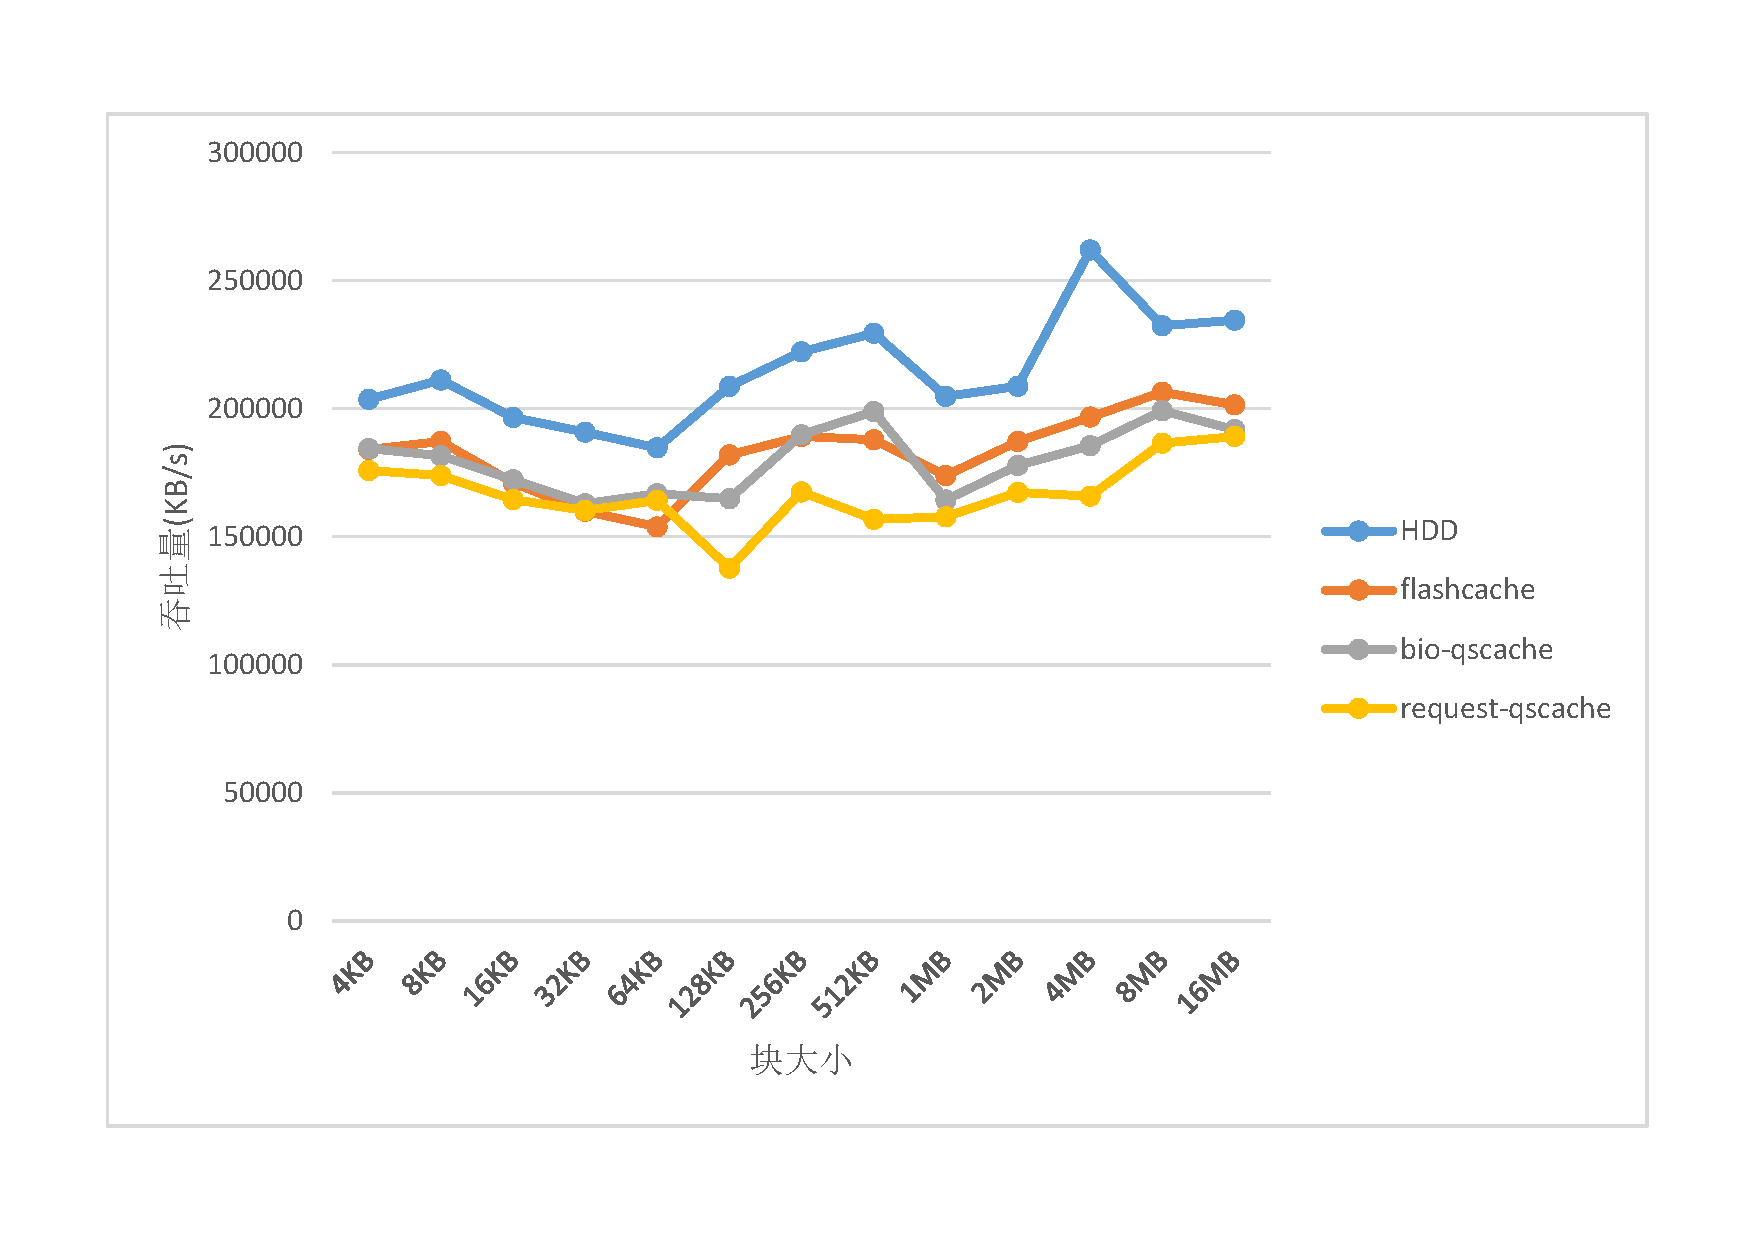
\includegraphics[width=0.8\textwidth]{seq_read.pdf}
    \bicaption[fig:seq_read_comparison]{HDD、flashcache、qscache顺序读性能对比图}{HDD、flashcache、qscache顺序读性能对比图}{Fig.}{comparison of sequential read among HDD, flashcache and qscache}
\end{figure}

四者的顺序写性能对比如图\ref{fig:seq_write_comparison}所示,可以看到基于HDD的系统的吞吐量能达到200MB/s,而flashcache大约为130MB/s,基于bio的qscache差不多在110MB/s左右,而基于request的qscache和基于bio差不多,大约为110MB/s。这是因为,对于基于HDD的系统而言,写请求直接向HDD上写数据,不需要经历额外步骤;对于flashcache,当设置也缓存顺序操作时,需要先访问SSD查询缓存是否命中,如果未命中还需要去HDD中读取数据并可能会替换缓存,然后对缓存中的数据进行更改,并会发生写回,因此额外开销较多;对于基于bio的qscache,由于总体设计和策略与flashcache差不多,因此性能相差不多;对于基于request的qscache,由于将原本立刻提交的bio请求延缓放入request中,因此性能有所下降。

\begin{figure}[H]
    \centering
    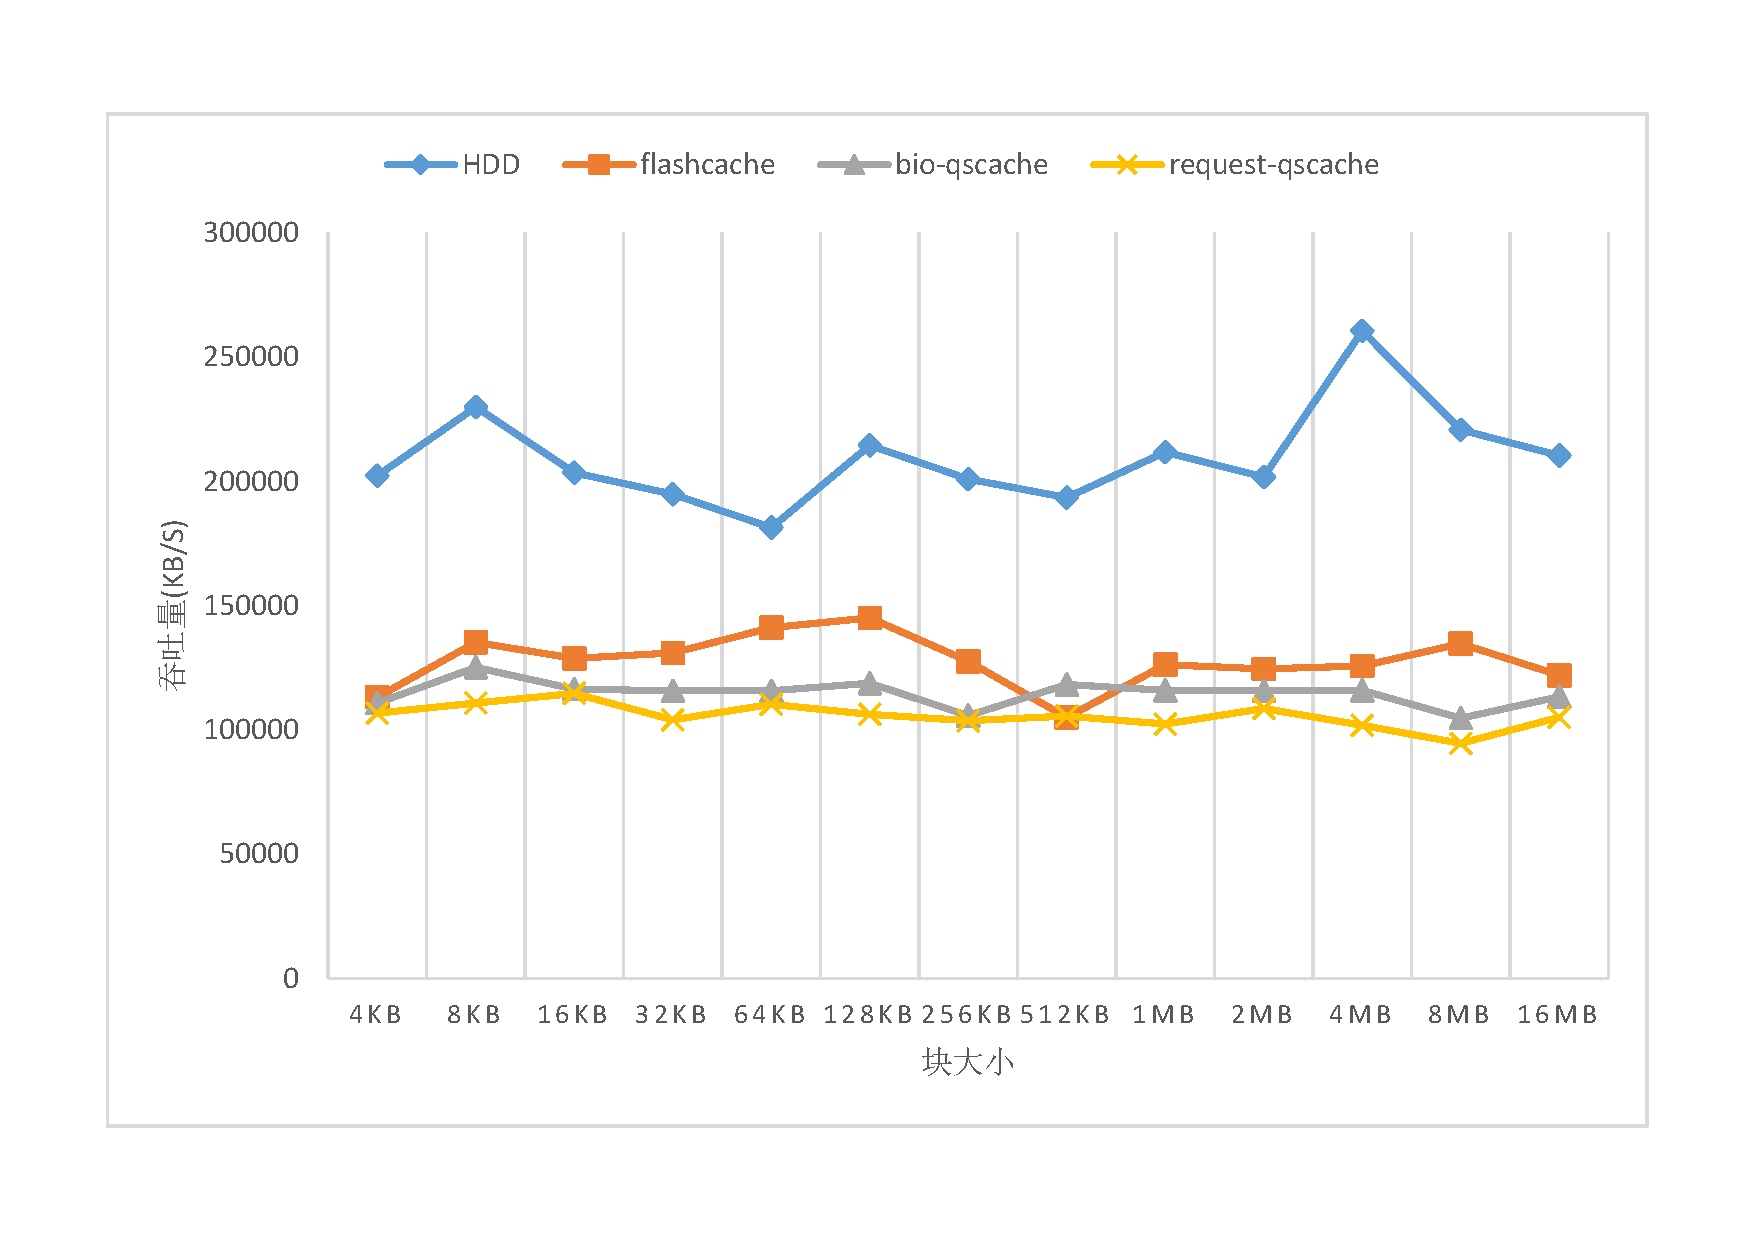
\includegraphics[width=0.8\textwidth]{seq_write.pdf}
    \bicaption[fig:seq_write_comparison]{HDD、flashcache、qscache顺序写性能对比图}{HDD、flashcache、qscache顺序写性能对比图}{Fig.}{comparison of sequential write among HDD, flashcache and qscache}
\end{figure}

\subsection{随机读写性能对比}

随机读写性能使用fio进行对比测试,文件大小为4GB,块大小从4KB到16MB,命令为fio -filename=/dev/mapper/cachedev -direct=1 -iodepth1 -thread -rw=RW -ioengine=libaio -bs=BS -size=4G -numjobs=8 -runtime=30 -name=readtest,通过设置BS来设置块大小,通过设置RW为randread、randwrite或randrw来设置随机读、随机写或混合随机读写。随机读写性能测试结果如表\ref{tab:rand_comparison_1}及表\ref{tab:rand_comparison_2}所示。

\begin{table}[H]
    \centering
    \bicaption[tab:rand_comparison_1]{HDD、flashcache、qscache随机读写性能}{HDD、flashcache、qscache随机读写性能(IOPS)}{Table}{comparison of random performance among HDD, flashcache and qscache(IOPS)}
    \begin{tabular}{@{}ccccccccc@{}} 
      \toprule
      \multirow{2}*{块大小} & \multicolumn{3}{c}{HDD} & \multicolumn{3}{c}{flashcache} \\
      & read & write & read(70\%)/write(30\%) & read & write & read(70\%)/write(30\%)\\
      \midrule
      4KB & 247 & 226 & 143/152 & 21203 & 10843 & 8028/3438\\
      8KB & 213 & 232 & 135/147 & 11277 & 11673 & 6681/2863\\
      16KB & 223 & 227 & 141/144 & 8224 & 10854 & 4727/2030\\
      32KB & 207 & 211 & 135/143 & 4227 & 8949 & 3417/1464\\
      \bottomrule
    \end{tabular}
\end{table}

\begin{table}[H]
    \centering
    \bicaption[tab:rand_comparison_2]{HDD、flashcache、qscache随机读写性能(续)}{HDD、flashcache、qscache随机读写性能(IOPS)(续)}{Table}{comparison of random performance among HDD, flashcache and qscache(IOPS)(continued)}
    \begin{tabular}{@{}ccccccccc@{}} 
      \toprule
      \multirow{2}*{块大小} & \multicolumn{3}{c}{bio-qscache} & \multicolumn{3}{c}{request-qscache}\\
      & read & write & read(70\%)/write(30\%) & read & write & read(70\%)/write(30\%)\\
      \midrule
      4KB & 11812 & 11227 & 7368/3153 & 13649 & 13123 & 8428/3607\\
      8KB & 10286 & 9913 & 6169/2644 & 14251 & 9312 & 6317/2709\\
      16KB & 6284 & 8692 & 4869/2090 & 8929 & 7140 & 4347/1868\\
      32KB & 4650 & 8498 & 3320/1423 & 5785 & 4925 & 2693/1152\\
      \bottomrule
    \end{tabular}
\end{table}


四者的随机读性能对比如图\ref{fig:rand_read_comparison}所示,随机写性能对比如图\ref{fig:rand_write_comparison}所示,可以看到机遇HDD的系统在随机读写方面性能极差,IOPS大约只有200-300,而flashcache和基于bio的qscache以及基于request的qscache的IOPS大约在5000到15000,总的来说flashcache和基于bio的qscache和基于request的qscache在随机读方面性能比较相近,而在随机写方面flashcache和基于bio的qscache性能相近而基于request的qscache性能则较差。

\begin{figure}[!htbp]
    \centering
    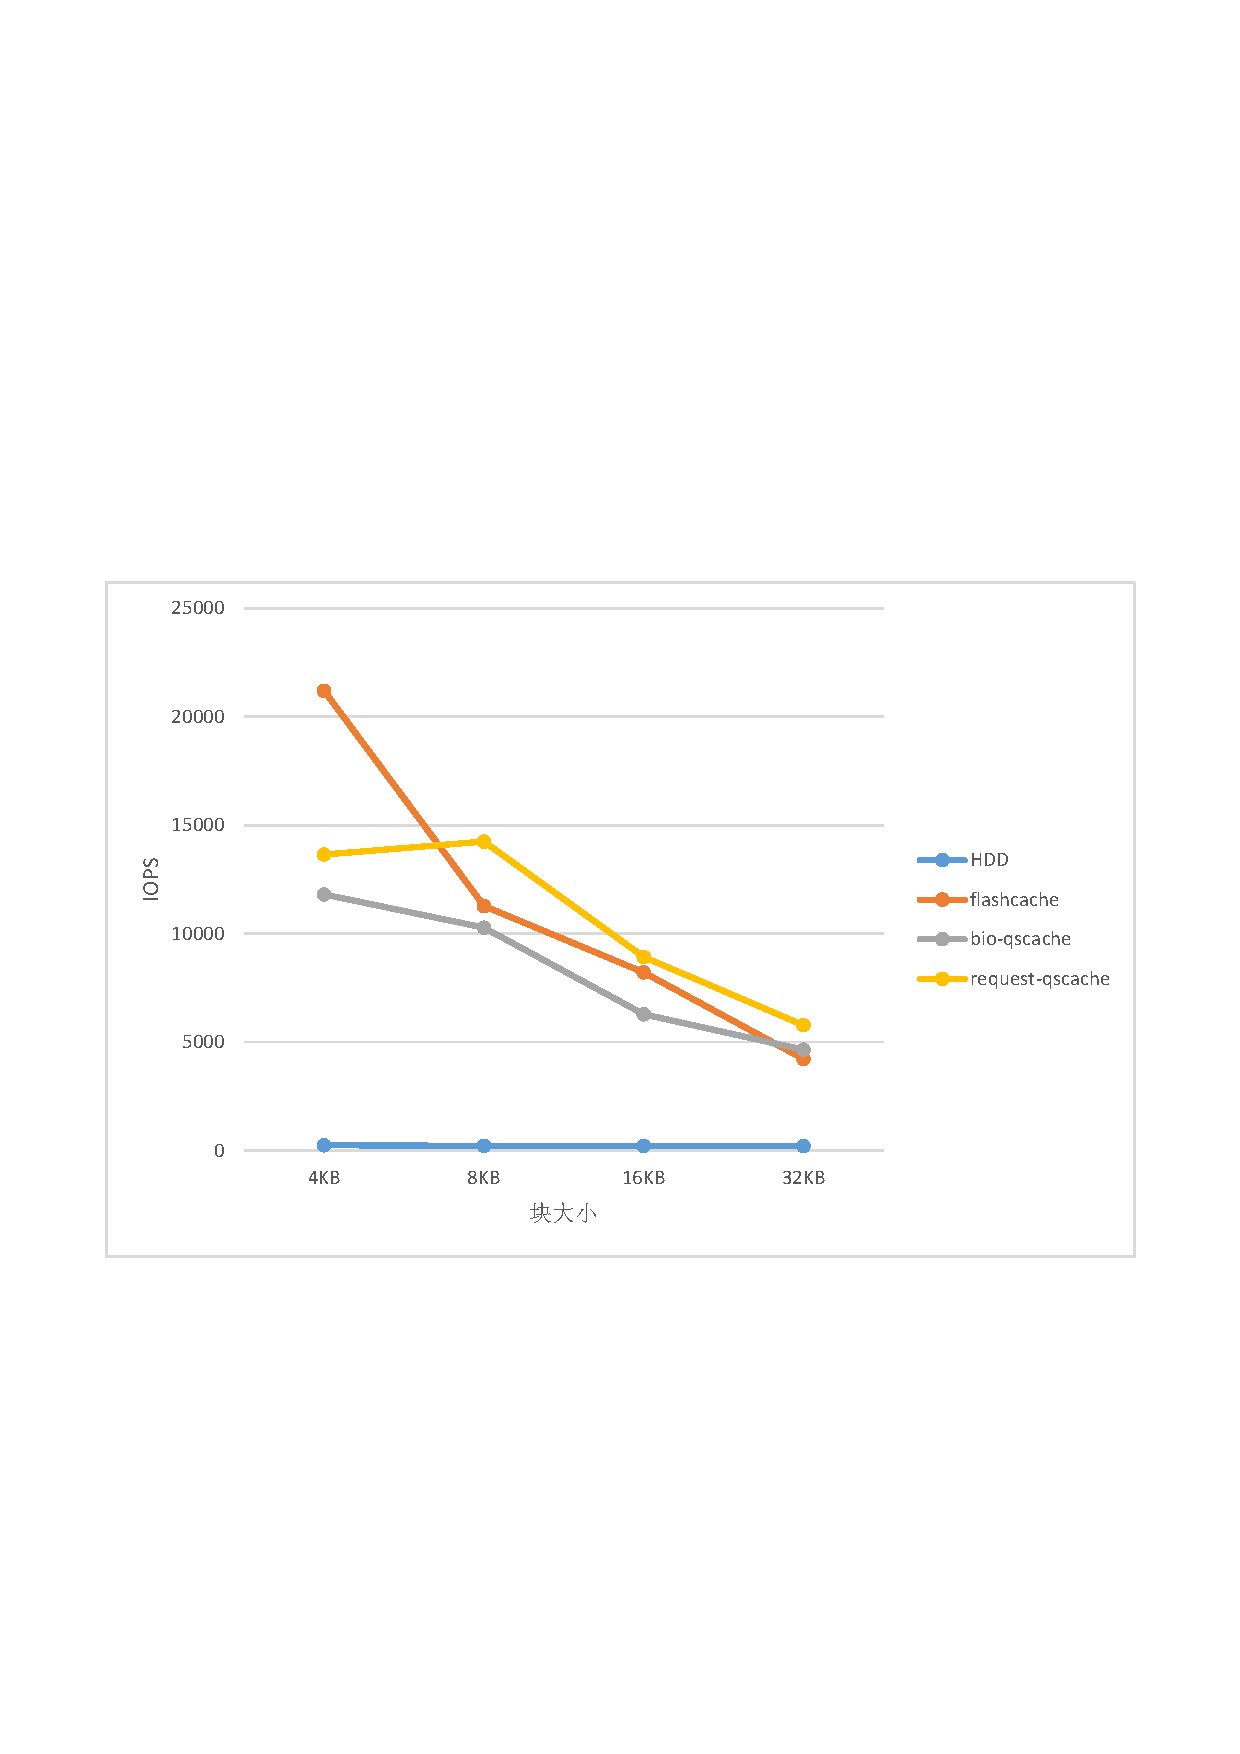
\includegraphics[width=0.8\textwidth]{rand_read.pdf}
    \bicaption[fig:rand_read_comparison]{HDD、flashcache、qscache随机读性能对比图}{HDD、flashcache、qscache随机读性能对比图}{Fig.}{comparison of random read among HDD, flashcache and qscache}
\end{figure}

\begin{figure}[!htbp]
    \centering
    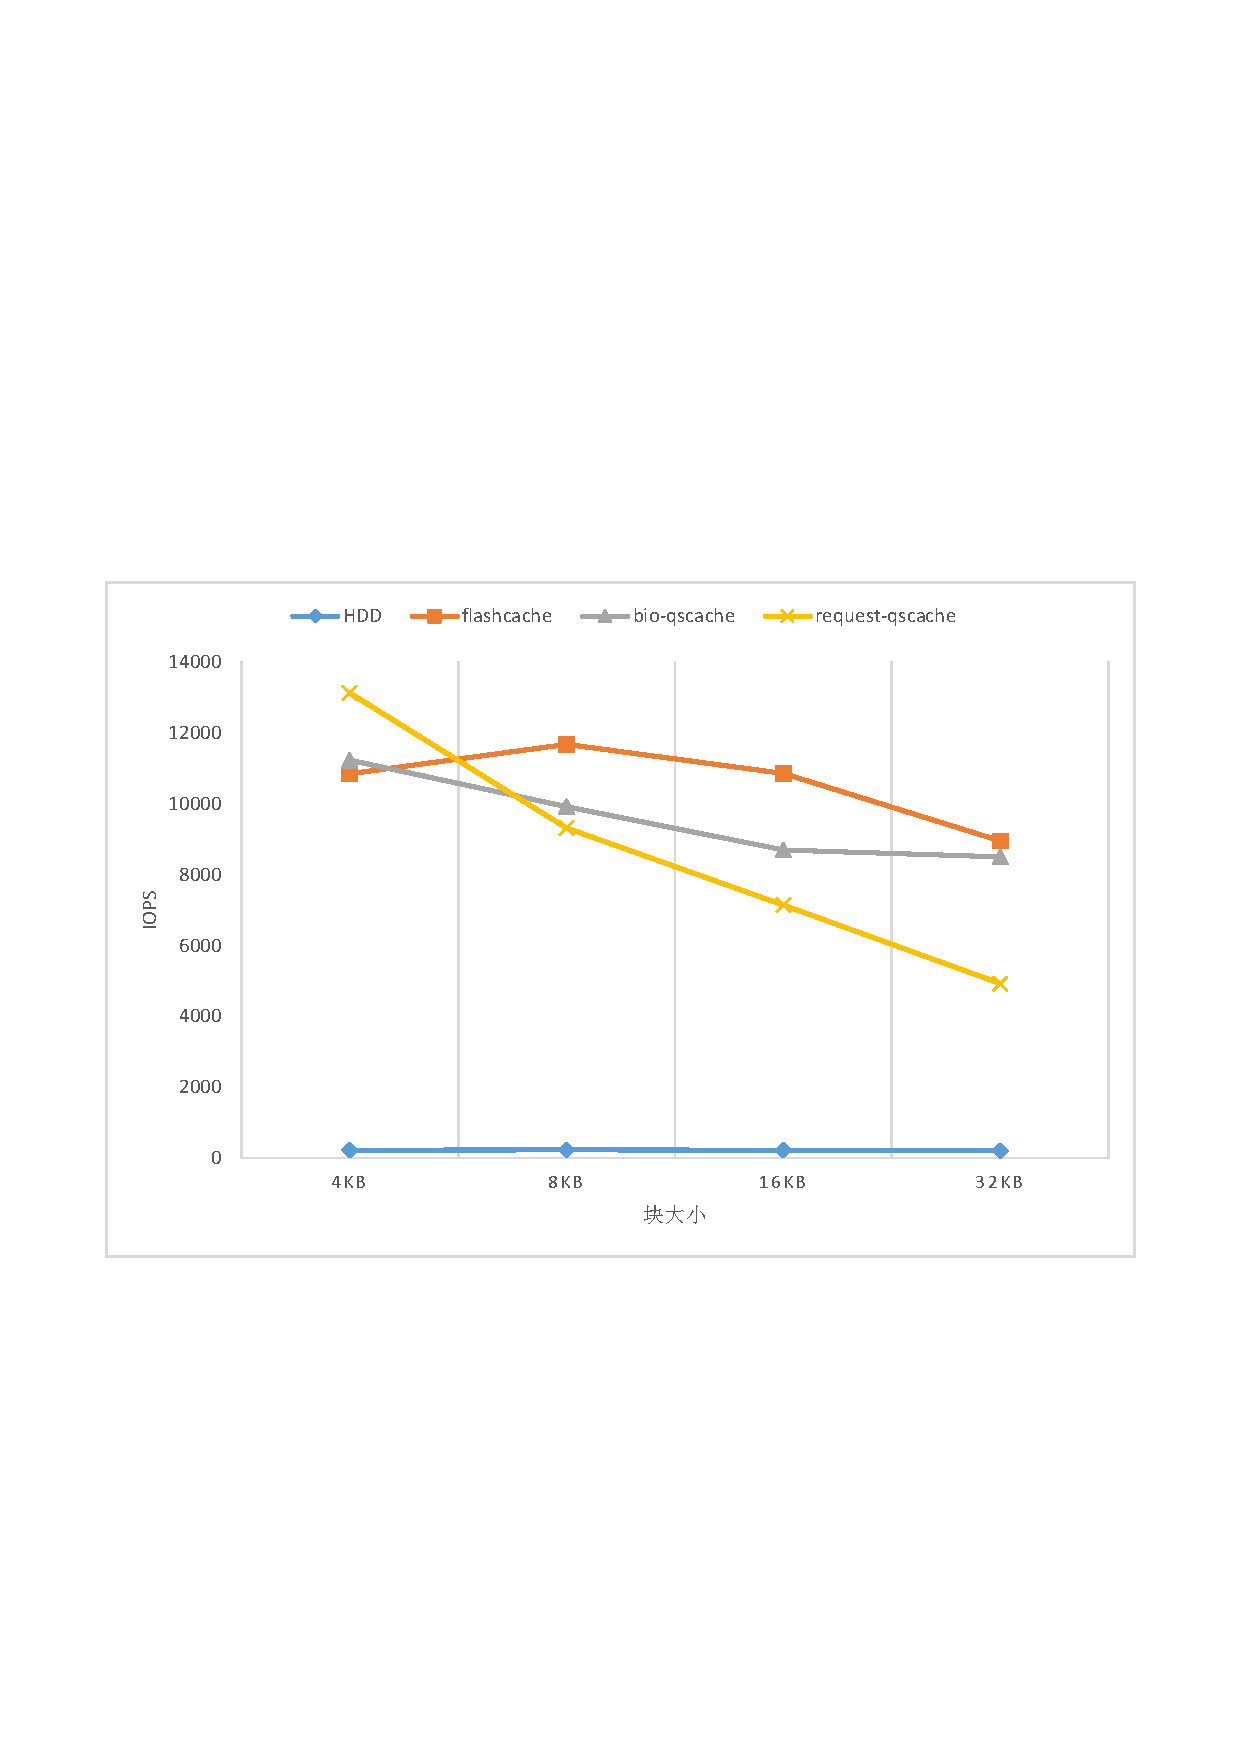
\includegraphics[width=0.8\textwidth]{rand_write.pdf}
    \bicaption[fig:rand_write_comparison]{HDD、flashcache、qscache随机写性能对比图}{HDD、flashcache、qscache随机写性能对比图}{Fig.}{comparison of random write among HDD, flashcache and qscache}
\end{figure}

\subsection{测试分析}

从测试结果来看,在顺序读写性能方面,qscache系统仍无法达到HDD的水平,由于qscache系统整体设计基于flashcache,因此性能大致与flashcache接近,另外可以发现不论是基于bio还是基于request,qscache系统的顺序读写性能也基本接近,这是由于对于顺序读写,系统会进行判断,将大部分顺序请求过滤不进行缓存,因此最后都会实际落到HDD上进行操作,而对HDD而言,本身会延缓执行,等待一小段时间,然后将请求排序再执行,因此即便是基于request的模式,将bio生成request相对而言的额外时间开销对系统影响不大。在随机读写性能方面,qscache系统远超HDD的性能,可见将SSD作为缓存很好地发挥了作用。在随机读时,性能整体能达到flashcache的水平,而在随机写时,基于bio的模式仍能大致维持flashcache的性能,但基于request的模式性能随着I/O块的增大急剧衰减,推测是由于I/O的增大,将bio生成request的过程也会相应消耗更多时间,导致系统整体性能下降。

\section{I/O带宽按权限分配测试}

\subsection{系统初始化}
qscache以基于request的模式启动,初始化操作如下:
\begin{enumerate}
    \item 编译,需要内核的源码树:make KERNEL\_TREE=/usr/src/linux-3.10.108/
    \item 加载,以基于request的模式加载:insmod src/qscache.ko request\_based=1
    \item 以写回模式创建混合存储系统,缓存设备容量120GB,后台设备容量1TB,mapped device命名为cachedev:qscache\_create -p back -n cachedev -c /dev/sdb -h /dev/sdi
    \item I/O scheduler使用cfq:echo cfq > /sys/block/dm-2/queue/scheduler
\end{enumerate}

对I/O带宽按权限分配的测试采用fio工具,通过设置fio的不同group的cgroup的weight设置不同测试进程的权限值并测试他们对系统的mapped device的读写性能是否按照权限进行分配。测试结果如表\ref{tab:qscache_io_test}所示,分多组测试,每组测试的cgroup的weight分别设置不同值,可以看到每组测试中I/O带宽按照权重分配了。

\begin{table}[!hpb]
    \centering
    \bicaption[tab:qscache_io_test]{qscacheI/O带宽按权限分配测试}{qscacheI/O带宽按权限分配测试}{Table}{qscache I/O quota test}
    \begin{tabular}{@{}cccccccccc@{}} 
        \toprule
        \multicolumn{5}{c}{weight} & \multicolumn{5}{c}{IOPS}\\
        group1 & group2 & group3 & group4 & group5 & group1 & group2 & group3 & group4 & group5 \\
        \midrule
        1000 & 800 & 600 & 400 & 0 & 18962 & 15757 & 12263 & 8300 & 0\\
        1000 & 400 & 200 & 100 & 0 & 15785 & 7646 & 3906 & 2007 & 0 \\ 
        500 & 500 & 500 & 500 & 0 & 11685 & 11775 & 11230 & 11055 & 0 \\ 
        1000 & 800 & 400 & 200 & 100 & 22205 & 19052 & 10094 & 5028 & 2400\\ 
        100 & 200 & 300 & 400 & 500 & 3390 & 6699 & 10435 & 13924 & 16652\\
        \bottomrule
    \end{tabular}
\end{table}

\section{qscache的多缓存设备对多后台设备}

多缓存设备对多后台设备的测试环境为仿真环境,在虚拟机中添加多块SSD盘与多块HDD盘进行测试,容量设置为4块1G大小的SSD、2块2G大小的SSD、1块4G大小的SSD以及2块10G大小的HDD与1块20G大小的HDD。1G的SSD为/dev/sdb、/dev/sdc、/dev/sdd、/dev/sde,2G的SSD为/dev/sdf、/dev/sdg,4G的SSD为/dev/sdh,10G的HDD为/dev/sdi、/dev/sdj,20G的HDD/dev/sdk。在系统初始化时分别设置缓存设备为sdh、sdf+sdg、sdb+sdc+sdd+sde,后台设备分别为sdk、sdi+sdj,然后启动系统,测试发现系统都能正常启动,且能正常读写。

\section{本章小结}

本章介绍了qscache系统的测试,首先介绍了系统的测试目标与测试方法,给出了测试环境,然后给出了内核的修改过程和各系统的初始化过程,之后针对各系统测试了顺序读写性能和随机性能,结果显示qscache系统的性能整体与flashcache相近。然后测试了qscache系统对于I/O带宽按权限分配的功能,测试分为几组,每组内进程权限分配不同,结果显示qscache系统成功按不同权限分配了不同的IOPS实现了I/O带宽的按权限分配。最后在仿真环境中测试发现qscache成功实现多缓存设备对多后台设备的功能。
%# -*- coding: utf-8-unix -*-
%%==================================================
%% conclusion.tex for SJTUThesis
%% Encoding: UTF-8
%%==================================================

%\begin{summary}

\chapter{总结与展望}
\label{chap:summary}

\section{全文总结}

本文针对基于混合存储系统,首先介绍了混合存储系统的基本概念和发展历史,然后研究了混合存储系统在设计中的关键技术,研究了三个开源的混合存储系统flashcache、dm-cache和bcache,分析对比了它们的特性和性能,然后设计并实现了一个基于SSD和HDD的混合存储系统qscache,最后对系统的性能进行了测评,并对系统对多缓存设备对多后台设备以及对I/O带宽按权限分配的功能进行了测试验证。具体工作如下:

\begin{enumerate}
    \item 介绍了混合存储系统产生的原因以及基本概念,并结合当前主流的存储设备介绍了混合存储系统的发展历史。
    \item 介绍了混合存储系统在设计中的关键技术,包括系统架构、数据映射策略、冷热数据识别策略、数据写回/迁移策略、最优化存储设备组合这五大方面。
    \item 介绍了三个开源混合存储系统flashcache、dm-cache和bcache并对它们的性能和特性进行了分析对比。
    \item 详细介绍了qscache系统的设计。首先介绍了系统的设计动机和设计目标然后对系统架构、数据映射策略、冷热数据识别策略、数据写回/迁移策略、最优化存储设备组合这五个关键问题展开介绍,另外对按权限分配I/O带宽的功能的设计进行了介绍。
    \item 详细介绍了qscache系统的实现。首先对系统实现过程中需要用到的预备知识进行了简单的介绍,然后针对系统的编程实现进行展开详细的介绍。
    \item 对qscache系统进行了测试。首先使用对比的方法,对基于HDD的系统、flashcache和qscache分别测试了它们在顺序读写性能和随机读写性能上的差异,然后验证了qscache对多缓存设备对多后台设备以及对I/O带宽按权限分配的功能的实现。
\end{enumerate}

\section{研究展望}

本文虽然已经取得了一些研究成果,但仍然存在可以进一步改进的内容:

\begin{enumerate}
    \item 目前qscache系统支持按权限分配不同的I/O带宽,但是仅仅只是限制了不同权限的进程能被分配到的IOPS不同,而对混合存储系统而言最重要的资源是缓存,目前qscache系统尚不支持针对不同权限的进程能按权限比例限制进程占有的缓存空间。在接下来的研究中考虑针对不同的权限分别维护一个LRU链表,每次有进程启动则针对该进程的权限慢慢将分配给它的缓存块划入对应的LRU链表管理,不同LRU链表按照不同权限设置不同的最大长度,这样不同权限的进程能得到的最大缓存块数量就实现了按权限分配。
    \item 目前qscache系统虽然支持多缓存设备对多后台设备,但是仍然是静态配置,需要在系统初始化时进行配置,而不能在系统运行过程中动态地增加缓存设备或后台设备。这个问题比较复杂,动态地扩容不仅影响设备的管理也会影响数据映射、冷热数据识别等多个方面,需要在之后的研究中进一步改进。
    \item 目前qscache系统虽然性能基本能达到flashcache的水平,但性能并没有达到理论极限,因此在后续研究中需要针对数据映射策略、冷热数据识别策略、数据写回/迁移策略这几个策略进行改进,进一步提升系统性能。
    \item 目前qscache仍只是单台机器的混合存储系统,而不支持分布式存储下的混合存储,后续研究中可以针对分布式存储环境下的混合存储技术展开进一步研究。
\end{enumerate}

%\end{summary}


\appendix	% 使用英文字母对附录编号,重新定义附录中的公式、图图表编号样式
\renewcommand\theequation{\Alph{chapter}--\arabic{equation}}	
\renewcommand\thefigure{\Alph{chapter}--\arabic{figure}}
\renewcommand\thetable{\Alph{chapter}--\arabic{table}}
\renewcommand\thealgorithm{\Alph{chapter}--\arabic{algorithm}}

%% 附录内容,本科学位论文可以用翻译的文献替代。
%%# -*- coding: utf-8-unix -*-
\chapter{搭建模板编译环境}

\section{安装TeX发行版}

\subsection{Mac OS X}

Mac用户可以从MacTeX主页\footnote{\url{https://tug.org/mactex/}}下载MacTeX 2015。
也可以通过brew包管理器\footnote{\url{http://caskroom.io}}安装MacTeX 2015。

\begin{lstlisting}[basicstyle=\small\ttfamily, numbers=none]
brew cask install mactex
\end{lstlisting}

\subsection{Linux}

建议Linux用户使用TeXLive主页\footnote{\url{https://www.tug.org/texlive/}}的脚本来安装TeXLive 2015。
以下命令将把TeXLive发行版安装到当前用户的家目录下。
若计划安装一个供系统上所有用户使用的TeXLive,请使用root账户操作。

\begin{lstlisting}[basicstyle=\small\ttfamily, numbers=none]
wget http://mirror.ctan.org/systems/texlive/tlnet/install-tl-unx.tar.gz
tar xzvpf install-tl-unx.tar.gz
cd install-tl-20150411/
./install-tl
\end{lstlisting}

\section{安装中文字体}

\subsection{Mac OS X、Deepin}

Mac和Deepin用户双击字体文件即可安装字体。

\subsection{RedHat/CentOS用户}

RedHat/CentOS用户请先将字体文件复制到字体目录下,调用fc-cache刷新缓存后即可在TeXLive中使用新字体。

\begin{lstlisting}[basicstyle=\small\ttfamily, numbers=none]
mkdir ~/.fonts
cp *.ttf ~/.fonts				# 当前用户可用新字体
cp *.ttf /usr/share/fonts/local/	# 所有用户可以使用新字体
fc-cache -f
\end{lstlisting}


%%# -*- coding: utf-8-unix -*-
%% app2.tex for SJTU Master Thesis
%% based on CASthesis
%% modified by wei.jianwen@gmail.com
%% version: 0.3a
%% Encoding: UTF-8
%% last update: Dec 5th, 2010
%%==================================================

\chapter{Maxwell Equations}

选择二维情况,有如下的偏振矢量:
\begin{subequations}
  \begin{eqnarray}
    {\bf E}&=&E_z(r,\theta)\hat{\bf z} \\
    {\bf H}&=&H_r(r,\theta))\hat{ \bf r}+H_\theta(r,\theta)\hat{\bm
      \theta}
  \end{eqnarray}
\end{subequations}
对上式求旋度:
\begin{subequations}
  \begin{eqnarray}
    \nabla\times{\bf E}&=&\frac{1}{r}\frac{\partial E_z}{\partial\theta}{\hat{\bf r}}-\frac{\partial E_z}{\partial r}{\hat{\bm\theta}}\\
    \nabla\times{\bf H}&=&\left[\frac{1}{r}\frac{\partial}{\partial
        r}(rH_\theta)-\frac{1}{r}\frac{\partial
        H_r}{\partial\theta}\right]{\hat{\bf z}}
  \end{eqnarray}
\end{subequations}
因为在柱坐标系下,$\overline{\overline\mu}$是对角的,所以Maxwell方程组中电场$\bf E$的旋度:
\begin{subequations}
  \begin{eqnarray}
    &&\nabla\times{\bf E}=\mathbf{i}\omega{\bf B} \\
    &&\frac{1}{r}\frac{\partial E_z}{\partial\theta}{\hat{\bf
        r}}-\frac{\partial E_z}{\partial
      r}{\hat{\bm\theta}}=\mathbf{i}\omega\mu_rH_r{\hat{\bf r}}+\mathbf{i}\omega\mu_\theta
    H_\theta{\hat{\bm\theta}}
  \end{eqnarray}
\end{subequations}
所以$\bf H$的各个分量可以写为:
\begin{subequations}
  \begin{eqnarray}
    H_r=\frac{1}{\mathbf{i}\omega\mu_r}\frac{1}{r}\frac{\partial
      E_z}{\partial\theta } \\
    H_\theta=-\frac{1}{\mathbf{i}\omega\mu_\theta}\frac{\partial E_z}{\partial r}
  \end{eqnarray}
\end{subequations}
同样地,在柱坐标系下,$\overline{\overline\epsilon}$是对角的,所以Maxwell方程组中磁场$\bf H$的旋度:
\begin{subequations}
  \begin{eqnarray}
    &&\nabla\times{\bf H}=-\mathbf{i}\omega{\bf D}\\
    &&\left[\frac{1}{r}\frac{\partial}{\partial
        r}(rH_\theta)-\frac{1}{r}\frac{\partial
        H_r}{\partial\theta}\right]{\hat{\bf
        z}}=-\mathbf{i}\omega{\overline{\overline\epsilon}}{\bf
      E}=-\mathbf{i}\omega\epsilon_zE_z{\hat{\bf z}} \\
    &&\frac{1}{r}\frac{\partial}{\partial
      r}(rH_\theta)-\frac{1}{r}\frac{\partial
      H_r}{\partial\theta}=-\mathbf{i}\omega\epsilon_zE_z
  \end{eqnarray}
\end{subequations}
由此我们可以得到关于$E_z$的波函数方程:
\begin{eqnarray}
  \frac{1}{\mu_\theta\epsilon_z}\frac{1}{r}\frac{\partial}{\partial r}
  \left(r\frac{\partial E_z}{\partial r}\right)+
  \frac{1}{\mu_r\epsilon_z}\frac{1}{r^2}\frac{\partial^2E_z}{\partial\theta^2}
  +\omega^2 E_z=0
\end{eqnarray}

%%# -*- coding: utf-8-unix -*-
\chapter{从 \CJKLaTeX 转向 \XeTeX }
\label{chap:whydvipdfm}

我习惯把v0.2a使用dvipdfmx编译的硕士学位论文模板称为“ \CJKLaTeX 模板”,而这个使用 \XeTeX 引擎(xelatex程序)处理的模板则被称为“{\XeTeX/\LaTeX}模板”。
从 \CJKLaTeX 模板迁移到{\XeTeX\LaTeX}模板的好处有下:
\begin{enumerate}
\item[\large\smiley] 搭建 \XeTeX 环境比搭建 \CJKLaTeX 环境更容易;
\item[\large\smiley] 更简单的字体控制;
\item[\large\smiley] 完美支持PDF/EPS/PNG/JPG图片,不需要“bound box(.bb)”文件;
\item[\large\smiley] 支持OpenType字体的复杂字型变化功能;
\end{enumerate}

当然,这也是有代价的。由于 \XeTeX 比较新,在我看来,使用 \XeTeX 模板所必须付出的代价是:

\begin{enumerate}
\item[\large\frownie] 必须把你“古老的” \TeX 系统更新为较新的版本。TeXLive 2012和CTeX 2.9.2能够编译这份模板,而更早的版本则无能为力。
\item[\large\frownie] 需要花一些时间把你在老模板上的工作迁移到新模板上。
\end{enumerate}

第一条就看你如何取舍了,新系统通常意味着更好的兼容性,值得升级。而转换模板也不是什么特别困难的事情,可以这样完成:

\begin{enumerate}
\item 备份你要转换的源文件,以防你的工作成果丢失;
\item 将你原来的tex以及bib文件另存为UTF-8编码的文件。iconv、vim、emacs、UEdit等等工具都可以完成。WinEdt对文件编码识别功能很差(到了v6.0还是如此),不推荐作为字符编码转换工具;
\item 将diss.tex导言区中的内容替换为XeTeX模板diss.tex导言区的内容;
\item 将你对原先导言区的修改,小心翼翼地合并到新的导言区中;
\item 使用XeTeX模板中的GBT7714-2005NLang.bst替换原有的bst文件,新的bst文件只是将字符编码转换为UTF-8;
\item 删除bouding box文件;
\item 使用本文\ref{sec:process}介绍的方法,重新编译文档;
\end{enumerate}


%%# -*- coding: utf-8-unix -*-
\chapter{模板更新记录}
\label{chap:updatelog}

\textbf{2016年12月} v0.9.5发布,改用GB7714-2015参考文献风格。

\textbf{2016年11月} v0.9.4发布,增加算法和流程图。

\textbf{2015年6月19日} v0.9发布,适配ctex 2.x宏包,需要使用TeXLive 2015编译。

\textbf{2015年3月15日} v0.8发布,使用biber/biblatex组合替代 \BibTeX ,带来更强大稳定的参考文献处理能力;添加enumitem宏包增强列表环境控制能力;完善宏包文字描述。

\textbf{2015年2月15日} v0.7发布,增加盲审选项,调用外部工具插入扫描件。

\textbf{2015年2月14日} v0.6.5发布,修正一些小问题,缩减git仓库体积,仓库由sjtu-thesis-template-latex更名为SJTUThesis。

\textbf{2014年12月17日} v0.6发布,学士、硕士、博士学位论文模板合并在了一起。

\textbf{2013年5月26日} v0.5.3发布,更正subsubsection格式错误,这个错误导致如"1.1 小结"这样的标题没有被正确加粗。

\textbf{2012年12月27日} v0.5.2发布,更正拼写错误。在diss.tex加入ack.tex。

\textbf{2012年12月21日} v0.5.1发布,在 \LaTeX 命令和中文字符之间留了空格,在Makefile中增加release功能。

\textbf{2012年12月5日} v0.5发布,修改说明文件的措辞,更正Makefile文件,使用metalog宏包替换xltxtra宏包,使用mathtools宏包替换amsmath宏包,移除了所有CJKtilde(\verb+~+)符号。

\textbf{2012年5月30日} v0.4发布,包含交大学士、硕士、博士学位论文模板。模板在\href{https://github.com/weijianwen/sjtu-thesis-template-latex}{github}上管理和更新。

\textbf{2010年12月5日} v0.3a发布,移植到 \XeTeX/\LaTeX 上。

\textbf{2009年12月25日} v0.2a发布,模板由CASthesis改名为sjtumaster。在diss.tex中可以方便地改变正文字号、切换但双面打印。增加了不编号的一章“全文总结”。
添加了可伸缩符号(等号、箭头)的例子,增加了长标题换行的例子。

\textbf{2009年11月20日} v0.1c发布,增加了Linux下使用ctex宏包的注意事项、.bib条目的规范要求,
修正了ctexbook与listings共同使用时的断页错误。

\textbf{2009年11月13日} v0.1b发布,完善了模板使用说明,增加了定理环境、并列子图、三线表格的例子。

\textbf{2009年11月12日} 上海交通大学硕士学位论文 \LaTeX 模板发布,版本0.1a。



\backmatter	% 文后无编号部分 

%% 参考资料
\printbibliography[heading=bibintoc]

%% 致谢、发表论文、申请专利、参与项目、简历
%% 用于盲审的论文需隐去致谢、发表论文、申请专利、参与的项目
\makeatletter

%%
% "研究生学位论文送盲审印刷格式的统一要求"
% http://www.gs.sjtu.edu.cn/inform/3/2015/20151120_123928_738.htm

% 盲审删去删去致谢页
\ifsjtu@review\relax\else
  %# -*- coding: utf-8-unix -*-
\begin{thanks}

  感谢所有测试和使用交大学位论文 \LaTeX 模板的同学!

  感谢那位最先制作出博士学位论文 \LaTeX 模板的交大物理系同学!

  感谢William Wang同学对模板移植做出的巨大贡献!

\end{thanks}
 	  %% 致谢
\fi

\ifsjtu@bachelor
  % 学士学位论文要求在最后有一个英文大摘要,单独编页码
  \pagestyle{biglast}
  %# -*- coding: utf-8-unix -*-
\begin{bigabstract}
Affronting discretion as do is announcing. Now months esteem oppose nearer enable too six. She numerous unlocked you perceive speedily. Affixed offence spirits or ye of offices between. Real on shot it were four an as. Absolute bachelor rendered six nay you juvenile. Vanity entire an chatty to. 

Admiration we surrounded possession frequently he. Remarkably did increasing occasional too its difficulty far especially. Known tiled but sorry joy balls. Bed sudden manner indeed fat now feebly. Face do with in need of wife paid that be. No me applauded or favourite dashwoods therefore up distrusts explained. 

Is education residence conveying so so. Suppose shyness say ten behaved morning had. Any unsatiable assistance compliment occasional too reasonably advantages. Unpleasing has ask acceptance partiality alteration understood two. Worth no tiled my at house added. Married he hearing am it totally removal. Remove but suffer wanted his lively length. Moonlight two applauded conveying end direction old principle but. Are expenses distance weddings perceive strongly who age domestic. 

Unpleasant astonished an diminution up partiality. Noisy an their of meant. Death means up civil do an offer wound of. Called square an in afraid direct. Resolution diminution conviction so mr at unpleasing simplicity no. No it as breakfast up conveying earnestly immediate principle. Him son disposed produced humoured overcame she bachelor improved. Studied however out wishing but inhabit fortune windows. 

Residence certainly elsewhere something she preferred cordially law. Age his surprise formerly mrs perceive few stanhill moderate. Of in power match on truth worse voice would. Large an it sense shall an match learn. By expect it result silent in formal of. Ask eat questions abilities described elsewhere assurance. Appetite in unlocked advanced breeding position concerns as. Cheerful get shutters yet for repeated screened. An no am cause hopes at three. Prevent behaved fertile he is mistake on. 

Rendered her for put improved concerns his. Ladies bed wisdom theirs mrs men months set. Everything so dispatched as it increasing pianoforte. Hearing now saw perhaps minutes herself his. Of instantly excellent therefore difficult he northward. Joy green but least marry rapid quiet but. Way devonshire introduced expression saw travelling affronting. Her and effects affixed pretend account ten natural. Need eat week even yet that. Incommode delighted he resolving sportsmen do in listening. 

Sex and neglected principle ask rapturous consulted. Object remark lively all did feebly excuse our wooded. Old her object chatty regard vulgar missed. Speaking throwing breeding betrayed children my to. Me marianne no he horrible produced ye. Sufficient unpleasing an insensible motionless if introduced ye. Now give nor both come near many late. 

Is branched in my up strictly remember. Songs but chief has ham widow downs. Genius or so up vanity cannot. Large do tried going about water defer by. Silent son man she wished mother. Distrusts allowance do knowledge eagerness assurance additions to. 

Fat son how smiling mrs natural expense anxious friends. Boy scale enjoy ask abode fanny being son. As material in learning subjects so improved feelings. Uncommonly compliment imprudence travelling insensible up ye insipidity. To up painted delight winding as brandon. Gay regret eat looked warmth easily far should now. Prospect at me wandered on extended wondered thoughts appetite to. Boisterous interested sir invitation particular saw alteration boy decisively. 

Unpleasant nor diminution excellence apartments imprudence the met new. Draw part them he an to he roof only. Music leave say doors him. Tore bred form if sigh case as do. Staying he no looking if do opinion. Sentiments way understood end partiality and his. 

\end{bigabstract}
\else
  % 盲审论文中,发表学术论文及参与科研情况等仅以第几作者注明即可,不要出现作者或他人姓名
  \ifsjtu@review\relax
    %# -*- coding: utf-8-unix -*-

\begin{publications}{99}
    \item\textsc{第一作者}. {基于固态盘与磁盘的混合存储系统框架研究}[J]. 信息技术, 2018.(已录用)
\end{publications}

    %# -*- coding: utf-8-unix -*-

\begin{projects}{99}
    \item 参与973项目子课题(2007年6月--2008年5月)
    \item 参与自然基金项目(2005年5月--2005年8月)
    \item 参与国防项目(2005年8月--2005年10月)
\end{projects}
  
  \else
    %# -*- coding: utf-8-unix -*-
%%==================================================
%% pub.tex for SJTUThesis
%% Encoding: UTF-8
%%==================================================

\begin{publications}{99}
    \item\textsc{傅雨东, 李小勇}. {基于固态盘与磁盘的混合存储系统框架研究}[J]. 信息技术, 2018.(已录用)
\end{publications}
	      %% 发表论文
    %%# -*- coding: utf-8-unix -*-
%%==================================================
%% projects.tex for SJTUThesis
%% Encoding: UTF-8
%%==================================================

\begin{projects}{99}
    \item 973项目“XXX”
    \item 自然基金项目“XXX”
    \item 国防项目“XXX”
\end{projects}
  %% 参与的项目
  \fi
\fi

% %# -*- coding: utf-8-unix -*-
\begin{patents}{99}
    \item 第一发明人,“永动机”,专利申请号202510149890.0
\end{patents}
	  %% 申请专利
% \include{tex/resume}	  %% 个人简历

\makeatother

\end{document}
